% Options for packages loaded elsewhere
\PassOptionsToPackage{unicode}{hyperref}
\PassOptionsToPackage{hyphens}{url}
%
\documentclass[
  letterpaper,
]{book}

\usepackage{amsmath,amssymb}
\usepackage{iftex}
\ifPDFTeX
  \usepackage[T1]{fontenc}
  \usepackage[utf8]{inputenc}
  \usepackage{textcomp} % provide euro and other symbols
\else % if luatex or xetex
  \usepackage{unicode-math}
  \defaultfontfeatures{Scale=MatchLowercase}
  \defaultfontfeatures[\rmfamily]{Ligatures=TeX,Scale=1}
\fi
\usepackage{lmodern}
\ifPDFTeX\else  
    % xetex/luatex font selection
\fi
% Use upquote if available, for straight quotes in verbatim environments
\IfFileExists{upquote.sty}{\usepackage{upquote}}{}
\IfFileExists{microtype.sty}{% use microtype if available
  \usepackage[]{microtype}
  \UseMicrotypeSet[protrusion]{basicmath} % disable protrusion for tt fonts
}{}
\makeatletter
\@ifundefined{KOMAClassName}{% if non-KOMA class
  \IfFileExists{parskip.sty}{%
    \usepackage{parskip}
  }{% else
    \setlength{\parindent}{0pt}
    \setlength{\parskip}{6pt plus 2pt minus 1pt}}
}{% if KOMA class
  \KOMAoptions{parskip=half}}
\makeatother
\usepackage{xcolor}
\setlength{\emergencystretch}{3em} % prevent overfull lines
\setcounter{secnumdepth}{5}
% Make \paragraph and \subparagraph free-standing
\ifx\paragraph\undefined\else
  \let\oldparagraph\paragraph
  \renewcommand{\paragraph}[1]{\oldparagraph{#1}\mbox{}}
\fi
\ifx\subparagraph\undefined\else
  \let\oldsubparagraph\subparagraph
  \renewcommand{\subparagraph}[1]{\oldsubparagraph{#1}\mbox{}}
\fi


\providecommand{\tightlist}{%
  \setlength{\itemsep}{0pt}\setlength{\parskip}{0pt}}\usepackage{longtable,booktabs,array}
\usepackage{calc} % for calculating minipage widths
% Correct order of tables after \paragraph or \subparagraph
\usepackage{etoolbox}
\makeatletter
\patchcmd\longtable{\par}{\if@noskipsec\mbox{}\fi\par}{}{}
\makeatother
% Allow footnotes in longtable head/foot
\IfFileExists{footnotehyper.sty}{\usepackage{footnotehyper}}{\usepackage{footnote}}
\makesavenoteenv{longtable}
\usepackage{graphicx}
\makeatletter
\def\maxwidth{\ifdim\Gin@nat@width>\linewidth\linewidth\else\Gin@nat@width\fi}
\def\maxheight{\ifdim\Gin@nat@height>\textheight\textheight\else\Gin@nat@height\fi}
\makeatother
% Scale images if necessary, so that they will not overflow the page
% margins by default, and it is still possible to overwrite the defaults
% using explicit options in \includegraphics[width, height, ...]{}
\setkeys{Gin}{width=\maxwidth,height=\maxheight,keepaspectratio}
% Set default figure placement to htbp
\makeatletter
\def\fps@figure{htbp}
\makeatother

\usepackage{booktabs}
\usepackage{caption}
\usepackage{longtable}
\usepackage{colortbl}
\usepackage{array}
\usepackage{makeidx}
\makeindex
\makeatletter
\@ifpackageloaded{bookmark}{}{\usepackage{bookmark}}
\makeatother
\makeatletter
\@ifpackageloaded{caption}{}{\usepackage{caption}}
\AtBeginDocument{%
\ifdefined\contentsname
  \renewcommand*\contentsname{Table of contents}
\else
  \newcommand\contentsname{Table of contents}
\fi
\ifdefined\listfigurename
  \renewcommand*\listfigurename{List of Figures}
\else
  \newcommand\listfigurename{List of Figures}
\fi
\ifdefined\listtablename
  \renewcommand*\listtablename{List of Tables}
\else
  \newcommand\listtablename{List of Tables}
\fi
\ifdefined\figurename
  \renewcommand*\figurename{Figure}
\else
  \newcommand\figurename{Figure}
\fi
\ifdefined\tablename
  \renewcommand*\tablename{Table}
\else
  \newcommand\tablename{Table}
\fi
}
\@ifpackageloaded{float}{}{\usepackage{float}}
\floatstyle{ruled}
\@ifundefined{c@chapter}{\newfloat{codelisting}{h}{lop}}{\newfloat{codelisting}{h}{lop}[chapter]}
\floatname{codelisting}{Listing}
\newcommand*\listoflistings{\listof{codelisting}{List of Listings}}
\usepackage{amsthm}
\theoremstyle{plain}
\newtheorem{theorem}{Theorem}[chapter]
\theoremstyle{remark}
\AtBeginDocument{\renewcommand*{\proofname}{Proof}}
\newtheorem*{remark}{Remark}
\newtheorem*{solution}{Solution}
\newtheorem{refremark}{Remark}[chapter]
\newtheorem{refsolution}{Solution}[chapter]
\makeatother
\makeatletter
\makeatother
\makeatletter
\@ifpackageloaded{caption}{}{\usepackage{caption}}
\@ifpackageloaded{subcaption}{}{\usepackage{subcaption}}
\makeatother
\ifLuaTeX
  \usepackage{selnolig}  % disable illegal ligatures
\fi
\usepackage[]{biblatex}
\addbibresource{references.bib}
\usepackage{bookmark}

\IfFileExists{xurl.sty}{\usepackage{xurl}}{} % add URL line breaks if available
\urlstyle{same} % disable monospaced font for URLs
\hypersetup{
  pdftitle={International Macroeconomics: Lecture Notes},
  pdfauthor={Udayan Roy},
  hidelinks,
  pdfcreator={LaTeX via pandoc}}

\title{International Macroeconomics: Lecture Notes}
\author{Udayan Roy}
\date{2024-11-02}

\begin{document}
\frontmatter
\maketitle

\renewcommand*\contentsname{Table of contents}
{
\setcounter{tocdepth}{2}
\tableofcontents
}
\mainmatter
\bookmarksetup{startatroot}

\chapter*{Preface}\label{preface}
\addcontentsline{toc}{chapter}{Preface}

\markboth{Preface}{Preface}

These lecture notes are for a very short course---roughly twelve
75-minute lectures---on international macroeconomics that I have taught
to junior and senior undergraduates. Although no prior knowledge of
economics is assumed, students typically come to the course after
completing courses on introductory microeconomics and macroeconomics.

This course is the second half of a one-semester course on international
economics, with the first half on international trade. The course's
textbook is \textcite{krugman2022international}. My goal here is simply
to present a concise version of chapters 13 through 18 of that book.

I had to grapple with some tough trade-offs because of the severe time
constraint. The core of the course is the theoretical framework
originally proposed by Robert A. Mundell\index{Mundell, Robert A.} and
J. Marcus Fleming\index{Fleming, J. Marcus}. I assume perfect capital
mobility\index{perfect capital mobility} throughout and, thereby, avoid
all discussion of wealth effects and portfolio theory.\footnote{On these
  issues, see \textcite{rodseth2000open}. By perfect capital
  mobility\index{perfect capital mobility} I mean a world in which (a)
  people who buy assets care only about the expected returns of those
  assets, and (b) they all have the same expectations about future
  changes in exchange rates. See section XXX.} I also assume a ``small''
country and, thereby, avoid the complex interactions of two-country
models. The perfect capital mobility and small country assumptions keep
this course very similar to the undergraduate macroeconomics course that
most of my students would have also taken. This simplicity, I think,
allows students to focus on the special aspects of \emph{international}
macroeconomics without having to learn a new kind of macroeconomics.

However, the discussion of expectations here may surprise even students
who have taken intermediate macroeconomics courses. I have broken up the
discussion of short-run analysis into separate chapters on permanent and
temporary changes in exogenous variables. Expectations are assumed to be
anchored to the long-run equilibrium outcome. This assumption is at the
root of the need to distinguish between temporary and permanent changes
in, say, fiscal policy. A temporary change affects neither the long-run
equilibrium outcome nor people's expectations, which are, after all,
assumed to be tied to the long-run equilibrium outcome. On the other
hand, a permanent change in, say, government spending affects the
long-run equilibrium level of the future value of the exchange rate and,
consequently, people's expectations about the future value of the
exchange rate. This change in expectations has short-run ramifications
that are absent in the analysis of temporary changes in government
spending.

These notions are present in \textcite{krugman2022international}, but
are not developed in a way that is clear enough and leisurely enough for
most students to grasp.\footnote{On page 442 of
  \textcite{krugman2022international} the authors address the issue as
  follows: ``A permanent policy shift affects not only the current value
  of the government's policy instrument (the money supply, government
  spending, or taxes) but also the \emph{long-run} exchange rate. This
  in turn affects expectations about future exchange rates. Because
  these changes in expectations have a major influence on the exchange
  rate prevailing in the short run, the effects of permanent policy
  shifts differ from those of temporary shifts.''} Other international
macroeconomics textbooks are no better in this respect, and usually a
lot worse.\footnote{Consider \textcite{feenstra2008international}. On
  page 551 of their excellent textbook, the authors write, ``{[}W{]}e
  can form expectations of the future exchange rate using the long-run
  monetary approach \ldots{}'' This easy-to-miss mention of the idea
  that expectations are based on the long-run equilibrium outcome is not
  adequately developed, as far as I am concerned. And the consequent
  need to distinguish between temporary and permanent policy changes is
  not as clearly developed as I would like.}

The role of the long-run outcome in anchoring expectations is also my
reason to discuss the long run before the short run. It would be
essentially impossible to do short-run analysis without some notion of
how expectations are formed, and the formation of expectations would be
impossible to explain without a discussion of long-run equilibrium.

These lecture notes are a work in progress. Please let me know if you
see any errors or if you see a way to make the book better. My mailing
address is Udayan Roy, College of Management, Long Island University,
Brookville, NY 11548, USA. My email address is
\href{mailto:udayan.roy@liu.edu}{\nolinkurl{udayan.roy@liu.edu}}.

\bookmarksetup{startatroot}

\chapter{Preliminaries}\label{sec-preliminaries}

\section{Economics}\label{sec-economics}

Economics\index{economics} is the study of how we---as individuals and
as societies---deal with the inescapable reality that ``we can't always
get what we want''. This fact of life, which economists call
\emph{scarcity}, makes it important for us to know how the many economic
variables that are important to us---such as the gross domestic product,
the unemployment rate, the consumer price index, etc.---can be made to
increase or decrease as needed. For example, scarcity makes it important
to understand whether our gross domestic product would increase or
decrease if we imposed tariffs on imported goods.

Economics consists of:

\begin{itemize}
\tightlist
\item
  \textbf{theories}, which are explanations---not necessarily
  proven---for the observed up and down movements of the economic
  variables that matter to us, and of
\item
  \textbf{statistical studies} that seek to test the reliability of
  economic theories.
\end{itemize}

\section{Macroeconomics}\label{sec-macro}

Macroeconomics\index{economics!macroeconomics} is the part of economics
that deals with economic variables that describe a country. When
describing the economy of the United States, an economist will probably
mention the gross domestic product, the unemployment rate, the inflation
rate, the trade deficit, etc., of the United States. These variables
that describe an entire country are at the heart of macroeconomics.
Macroeconomics consists of (a) theories that derive predictions about
the likely changes in such economic variables and (b) statistical
studies that scour history to check the predictive accuracy of the
theories.

\section{International Macroeconomics}\label{sec-intmac}

The macroeconomic behavior of a country that is economically isolated
from other countries---a \textbf{closed economy}, in the jargon of
economics---will not necessarily be the same as the macroeconomic
behavior of a highly globalized country---an \textbf{open economy}.
International macroeconomics is the part of macroeconomics that deals
with countries for which international economic links are important.
Such links may include international trade in goods and services,
cross-border migration of people, and cross-border borrowing and
lending.

\section{Why Study International Macroeconomics?}\label{sec-whyintmac}

The point of studying international macroeconomics is to be able to
\emph{evaluate alternative macroeconomic policies} and choose the one
that's best. If we have a reliable theory that explains the reasons why
a certain variable goes up or down, we might be able to figure out
policies that will move that variable in the desired direction. For
example, if we can figure out the reasons for the up and down movements
of a nation's trade deficit, we might be able to design economic
policies that drive the trade deficit in the desired direction, be it up
or down.

In discussing macroeconomic policy\index{policy} I will focus on
\textbf{fiscal policy} and \textbf{monetary policy}.

\subsection{What Is Fiscal Policy?}\label{sec-fiscal}

Fiscal policy\index{policy!fiscal policy} consists of all the methods of
controlling an economy by making changes to the government's budget. A
government's \textbf{budget}\index{budget, government's} is a
description of its spending and revenue-raising plans. So, for my
purposes, fiscal policy essentially consists of changes in total
\textbf{government spending}\index{government spending}, \(G\), and
\textbf{total tax revenue}\index{tax revenue}, \(T\).\footnote{First,
  note that I have begun to introduce symbols to denote economic
  variables. As you will see, the good part of the use of symbols is
  that it speeds up the discussion considerably. The bad part is that
  you will need to remember which symbol denotes which variable.}

Second, to be more precise, \(T\) represents total \emph{net} tax
revenue, which equals the tax revenues of the government less
\textbf{transfer payments} made by the government. Transfer payments are
gifts, such as cash grants to the poor.

Third, \(G\) represents government \emph{purchases} rather than
government spending. The latter includes the former plus transfer
payments, which, as I said in the previous paragraph, are gifts, not
payments made for purchases. \(G\) represents only what the government
spends for its purchases of goods and services.

\subsection{What Is Monetary Policy?}\label{sec-monetary}

Monetary policy\index{policy!monetary policy} consists of all the
methods of controlling an economy by making changes to the economic
variables that are directly controlled by the country's monetary
authorities, such as the Federal Reserve in the United States. For my
purposes, monetary policy consists of changes in a country's
\textbf{money supply}, \(M\). A central bank may print money and lend it
to financial institutions such as banks. If and when these financial
institutions in turn lend the money to people or to businesses, the
newly printed money begins to affect actual economic activity. This, of
course, is why the central bank printed the money in the first place.

\subsection{Monetary Unions}\label{sec-monetary-unions}

In the case of the 24 European countries that all use the same currency,
the euro, there is no monetary policy at all to conduct!\footnote{As of
  October 2023, the eurozone consists of 20 members who are European
  Union (EU) members and use the euro. They are Austria, Belgium,
  Croatia, Cyprus, Estonia, Finland, France, Germany, Greece, Ireland,
  Italy, Latvia, Lithuania, Luxembourg, Malta, the Netherlands,
  Portugal, Slovakia, Slovenia and Spain. The non-EU countries that use
  the euro are Andorra, Vatican City, and Monaco and San Marino.} These
countries have willingly given up their individual currencies and formed
a \textbf{monetary union}\index{European Monetary Union}. The monetary
policy of the entire eurozone is determined by the European Central
Bank\index{central banks!European Central Bank} in Frankfurt.\footnote{This
  lack of the ability to use monetary policy is also true of a handful
  of countries that have ``dollarized''\index{dollarization}. These are
  countries that have decided to use another country's currency as their
  own currency. For example, East Timor, Ecuador, El Salvador, and
  Panama use the U.S. dollar as their currency.}

It is important to understand the pros and cons of the formation of a
monetary union so that countries considering joining a monetary union
may make smart choices.

Just as multiple countries may choose to use a common currency, they may
also choose to adopt a common fiscal policy whereby a central budget
sets expenditure and revenue-raising rules for all members of the club.
For example, the USA may be thought of as a union of fifty states with a
common currency and a unified fiscal policy decided in Washington, D.C.
In fact, we will see that it may be difficult for a group of countries
to share a common currency and retain independent national fiscal
policies. During the economic crises that cascaded through several
eurozone countries---such as Ireland, Greece, and Spain---during
2009--2012, some commentators argued that the eurozone countries needed
to unify their budgets---and become something like a United States of
Europe---if they were to have a stable monetary union.

In any case, countries considering a monetary and/or fiscal union need
to be able to make their choices with their eyes wide open. It is,
therefore, necessary for international economics to have something
useful to say on the issue.

\bookmarksetup{startatroot}

\chapter{National Income Accounts, Prices, and
Inflation}\label{sec-niaccounts}

Recall from sections Section~\ref{sec-economics} --
Section~\ref{sec-intmac} that international macroeconomics consists of
explanations for the observed up-and-down movements of important
macroeconomic variables in a globalized (or, open) economy. This chapter
begins the task of defining some of those important macroeconomic
variables. This chapter also discusses certain accounting rules that
describe how certain important macroeconomic variables are related to
each other, simply by virtue of the way they are defined.

\section{National Income Accounts}\label{sec-nia}

The national income accounts of a country consist of data on variables
that tell us about the country's total production of goods and services,
and what those goods and services are being used for. An important
measure of the total production of goods and services is the gross
domestic product (GDP). If you look up a country's GDP data in a book or
on the Internet, you'll see that GDP data comes in two flavors, nominal
and real. Nominal GDP is discussed in the next section, and real GDP is
discussed in the section after that.

\section{Nominal Gross Domestic Product}\label{sec-nGDP}

\index{gross domestic product!nominal}

There are three equivalent ways of understanding nominal gross domestic
product: the value-added approach, the income approach, and the
expenditure approach.

\subsection{GDP: The Value-Added Approach}\label{sec-gdp-value-added}

The \textbf{value added}\index{value added} by a firm is the monetary
market value of the goods and services produced by the firm \emph{minus}
the monetary market value of the goods and services that the firm
purchases from other firms (for use in its own production, obviously). A
country's gross domestic product is then the total value added---during
a specified time period, such as a year---by all producers of for-sale
goods located within the country.

Consider a university. Let's say that the market value of the
educational services provided by this university was \$20 m during 2008,
as measured by the tuition paid by its students. It would be incorrect,
however, to say that the market value of the work done in the university
was \$20 m. The university used a lot of electricity that was produced
by some other firm. The university bought massive amounts of paper,
computer printer cartridges, and other stationery from other firms. The
university's capital equipment (which includes its buildings, its
computers, its fleet of cars and trucks, etc.) needed costly
replacements that had to be bought from other firms. Suppose the
monetary market value of these and all other goods and services that
were purchased from other firms and used by the university's employees
during 2008 was \$16 m. Then the value added by the university was only
\$20 m -- \$16 m = \$4 m.

And, as we saw two paragraphs back, \emph{the total value added by all
producers of for-sale goods and services located within a country's
borders is that country's gross domestic product}.

\subsection{GDP: The Income Approach}\label{sec-gdp-income}

Now, returning to our hypothetical university, a question arises: What
happens to the \$4 m that the university has left of its \$20 m tuition
revenues after paying \$16 m to other firms for its various purchases?
Where will this \$4 m go?

A big chunk will go to pay \textbf{wages} to the university's employees.
The university will have to pay \textbf{rent} on some property that it
had leased from others. It will have to pay \textbf{interest} to its
banks for the loans it had taken. It will have to pay what are called
\textbf{indirect business taxes} to the government. And whatever remains
will be the university's \textbf{profits}, which belong to the
university's owners or shareholders. In other words, the university's
value added ends up as the income of the owners of the resources
employed by the university.

What's true for this university is true for all firms in the country.
Therefore, as a country's gross domestic product is its total value
added, one can say that \emph{a country's gross domestic product is the
total income earned by the owners of all the resources employed by
producers located within the country's borders}.

\subsection{GDP: The Expenditure Approach}\label{sec-gdp-expenditure}

Let us consider our hypothetical university one more time. The education
it provides its students is an example of a \textbf{final
good}.\footnote{When I say ``good'', I mean ``good or service''.} A good
is called a final good when it is sold to its final user; a final user
is someone who will not use the purchased good to produce something else
for sale.

The electricity, paper, other stationery, etc., that the university buys
for the purpose of producing educational services are called
\textbf{intermediate goods}. When goods are bought by businesses from
other businesses, used as inputs in the production of other for-sale
goods, and, in the process, end up disappearing completely inside those
other goods, they are called intermediate
goods\index{goods!intermediate}. (Think of all the milk produced by U.S.
dairy farmers that disappear into the ice cream made by U.S. firms such
as Ben \& Jerry's.)

In my example, students paid \$20 m for education, the final good
produced by the university. As we saw in section
Section~\ref{sec-gdp-income} above, this money ends up as the incomes of
all the resources---employed by the university and by the firms from
which the university bought electricity, paper, and all sorts of other
intermediate goods---that were used to produce the final good,
education.

Extrapolating from this example, we can say that the total expenditure
on all final goods produced domestically and sold to domestic final
users---let's call these goods category \(a\) goods---is equal to the
income earned by all resources employed in the production of these final
goods and the intermediate goods used in the production of these final
goods.

Moreover, what's true for education must also be true for the domestic
production of all exported goods---let's call these category \(b\)
goods. The total expenditure on these goods must end up as the total
income of all resources used to make these goods and the intermediate
goods bought by the producers of these goods.

Therefore, the total expenditure on the goods in categories \(a\) and
\(b\) \emph{minus} the value of the intermediate goods imported by the
producers of category \(a\) and \(b\) goods is the total income of all
resources that were used to make category \(a\) and \(b\) goods and the
\emph{domestically produced} intermediate goods bought by their
producers.

But this income must be the total income of all resources employed in
domestic production. After all, any domestic producer would have to
produce either final goods sold to domestic buyers (category \(a\)), or
exported goods (category \(b\)), or the domestically produced
intermediate goods bought by category \(a\) and \(b\) producers.

Therefore, going by the definition of GDP in
Section~\ref{sec-gdp-income}, the total expenditure on category \(a\)
and \(b\) goods \emph{minus} imports of intermediate goods equals gross
domestic product.

In publications of government statistics, the total expenditure by
households residing within a country is called \textbf{personal
consumption expenditure} or, simply, consumption. The total spending on
final goods by domestic businesses is called \textbf{gross private
domestic investment} or, simply, investment. Total spending by domestic
government entities is called \textbf{government expenditure}.
Therefore, total expenditure on \emph{all} final goods by domestic
residents is consumption \(+\) investment \(+\) government spending.
Consequently, total expenditure on final goods produced domestically and
sold to domestic residents---category \(a\)---is consumption \(+\)
investment \(+\) government spending \(-\) imports of final goods.
Therefore, the total expenditure on goods in categories \(a\) and \(b\)
equals consumption \(+\) investment \(+\) government spending \(+\)
exports \(-\) imports of final goods. Therefore, recalling the last
sentence of the previous paragraph, gross domestic product equals
consumption \(+\) investment \(+\) government spending \(+\) exports
\(-\) imports of final goods \(-\) imports of intermediate goods.
Consequently, we get:

\begin{equation}\phantomsection\label{eq-gdp1}{
\text{GDP}=\text{Consumption}+\text{Investment}+\text{Government Purchases}+\text{Exports}-\text{Imports}.
}\end{equation}

This is easily the most important equation in this book. It is called
the \textbf{national income identity}\index{national income identity}
and will be central to our discussion right up to the very end of this
book.

Note that it is not terribly meaningful to distinguish between exports
of final goods and exports of intermediate goods. And the same can be
said about imports too. Nevertheless, if we simplify a bit and assume
that all exports and imports are of final goods, Equation~\ref{eq-gdp1}
can be interpreted as follows: a country's gross domestic product is the
market value of all final goods and services produced within the country
in a given period of time (usually a year). This is a very popular
definition that you will see in many textbooks. I will use this
definition in this book too, as a convenient shorthand.

\subsection{GDP: Overview}\label{sec-gdp-overview}

\captionsetup{labelsep=none}

\begin{longtable}{cccc}

\caption{\label{tbl-gdp-n-deflator}}

\tabularnewline

\caption*{
{\large USA, 2014 -- 2023}
} \\ 
\toprule
Year & Nominal GDP & Real GDP & GDP Deflator \\ 
\midrule\addlinespace[2.5pt]
2014 & 17608.14 & 18261.71 & 96.421 \\ 
2015 & 18295.02 & 18799.62 & 97.316 \\ 
2016 & 18804.91 & 19141.67 & 98.241 \\ 
2017 & 19612.10 & 19612.10 & 100.000 \\ 
2018 & 20656.52 & 20193.90 & 102.291 \\ 
2019 & 21539.98 & 20715.67 & 103.979 \\ 
2020 & 21354.10 & 20267.58 & 105.361 \\ 
2021 & 23681.17 & 21494.80 & 110.172 \\ 
2022 & 26006.89 & 22034.83 & 118.026 \\ 
2023 & 27720.71 & 22671.10 & 122.273 \\ 
\bottomrule

\end{longtable}

According to the Bureau of Economic Analysis of the U.S. Department of
Commerce, the nominal GDP of the United States for 2014 was \$17608.14
billion. This means that spending by US residents on the final goods and
services that were ``Made in USA'' in 2014 plus net exports of ``Made in
USA'' goods and services were together equal to a grand total of
\$17608.14 billion. This number is also the total value added by all
producers located in the USA. And---perhaps most meaningfully---this
number is the total income earned by all productive resources employed
by producers located in the USA.

\section{Real Gross Domestic Product}\label{sec-rGDP}

\index{gross domestic product!real}

Looking at the second column in Table~\ref{tbl-gdp-n-deflator}, we see
that the nominal gross domestic product of the United States increased
from \$17608.14 billion in 2014 to \$18295.02 billion in 2015 and to
\$18804.91 billion in 2016. If one assumes that our quality of life
depends crucially on the goods and services we produce, these ever
increasing dollar figures seem like good news.

But are they?

As nominal gross domestic product is the monetary market value of all
final goods produced, it could increase from one year to the next either
as a result of:

\begin{itemize}
\tightlist
\item
  increases in the production of various goods, or
\item
  increases in the market prices of those goods, or
\item
  increases in both production and prices.
\end{itemize}

Consequently, increases in nominal gross domestic product do not
necessarily imply increases in production. Mere inflation could make the
numbers go up and up.

Now if, by sheer luck, all prices remained unchanged during 2014 --
2016, then, yes, the increases in nominal GDP during that period would
indeed strongly indicate rising overall levels of production.\footnote{Even
  in this case, production might rise for some goods and fall for
  others. But it is straightforward to show that if nominal GDP rises
  and prices stay unchanged, a country would be able to buy increasing
  amounts of \emph{every} good through international trade.}

Of course, in real life, prices do not stay unchanged year after year.
But even if prices moved around a lot during 2014 -- 2016, we could
still ask a hypothetical question: What would nominal GDP have been
during 2014 -- 2016 if prices had remained unchanged at 2014 levels?
This is not an unanswerable question. We know the 2014 prices of all
final goods, and we know the quantities produced, of all final goods,
during the years 2014, 2015 and 2016. (Otherwise, we would not have been
able to calculate the nominal GDP figures in
Table~\ref{tbl-gdp-n-deflator}.) Therefore, we can easily calculate what
America's nominal GDP would have been in those years, had the prices of
2014 prevailed in all years.

Indeed, data on this hypothetical measure---formally called \textbf{real
gross domestic product} or \textbf{constant-prices gross domestic
product} or \textbf{inflation-adjusted gross domestic product}---is
available for virtually every country in the world. The third column of
Table~\ref{tbl-gdp-n-deflator} shows America's real gross domestic
product, calculated on the assumption that the prices of the year 2017
prevailed in all years, for the decade 2014-- 2023.\footnote{Formally,
  these numbers are in ``chained 2017 dollars''. The subtleties of this
  particular method of adjusting nominal values for inflation will not
  concern us here.}

As you can see, not only did America's nominal GDP increase throughout
2014-- 2023, so did \emph{real} GDP. This is clear evidence of actual
increases in production. To repeat, the dollar figures in the third
column of Table~\ref{tbl-gdp-n-deflator} were all calculated on the
hypothetical assumption that 2017's prices prevailed in every year. As
the same prices were used for every year's real GDP calculations, the
increases in real GDP strongly indicate overall increases in production.

The year whose prices are being assumed hypothetically to prevail in all
years---the year 2017 in this case---is called the \textbf{base year}.
There is nothing sacrosanct about the year 2017---any other year could
have served just as well. As long as every year's GDP is calculated
using the same set of prices, we will get a measure of GDP that is not
affected by fluctuations in the overall level of prices.

In the rest of this book, all references to gross domestic product are
references to \emph{real} gross domestic product. Also, I will use the
symbol \(Y\) to denote real gross domestic product.

\subsection{Notation: Growth Rates}\label{sec-notngrowth}

Consider a variable \(x\). I will denote its \emph{current value} as
simply \(x\) and its \emph{past value} as \(x_{-1}\). Then, the
\emph{growth rate} of \(x\), which I will denote \(x_g\), can be defined
as follows: \begin{equation}\phantomsection\label{eq-growthrate}{
x_g\equiv\frac{x-x_{-1}}{x_{-1}}.
}\end{equation}

Here, \(x-x_{-1}\) represents the increase in the value of \(x\).
Therefore, \((x-x_{-1})/x_{-1}\) is the proportionate increase in the
value of \(x\) or, simply, the growth rate of \(x\). If \(x_{-1}=50\)
and \(x=60\), the increase is \(x-x_{-1}=60-50=10\). But the rate of
growth is \(x_g\equiv(x-x_{-1})/x_{-1}=(60-50)/50=0.20\).

If you want the growth rate \emph{as a percentage}, simply multiply
\(x_g\) by 100 to get \(0.20\times100=20\) percent.

\captionsetup{labelsep=none}

\begin{longtable}{cccc}

\caption{\label{tbl-growth-inflation}}

\tabularnewline

\caption*{
{\large USA, 2014 -- 2023}
} \\ 
\toprule
Year & Growth, Nominal GDP (\%) & Growth, Real GDP (\%) & Inflation (\%) \\ 
\midrule\addlinespace[2.5pt]
2014 & $4.31$ & $2.52$ & $1.74$ \\ 
2015 & $3.90$ & $2.95$ & $0.93$ \\ 
2016 & $2.79$ & $1.82$ & $0.95$ \\ 
2017 & $4.29$ & $2.46$ & $1.79$ \\ 
2018 & $5.33$ & $2.97$ & $2.29$ \\ 
2019 & $4.28$ & $2.58$ & $1.65$ \\ 
2020 & $-0.86$ & $-2.16$ & $1.33$ \\ 
2021 & $10.90$ & $6.06$ & $4.57$ \\ 
2022 & $9.82$ & $2.51$ & $7.13$ \\ 
2023 & $6.59$ & $2.89$ & $3.60$ \\ 
\bottomrule

\end{longtable}

To take a more concrete example, consider real gross domestic product
(\(Y\)) and its growth rate (\(Y_g\)). Table~\ref{tbl-gdp-n-deflator}
tells us that real GDP of the U.S. (in billions of chained 2017
dollars), was \$18261.71 in 2014 and \$18799.62 in 2015. Therefore, the
growth rate of America's real GDP in 2015 was \[
Y_{g,2015}=\frac{Y_{2015}-Y_{2014}}{Y_{2014}} = \frac{18799.62-18261.71}{18261.71}\times 100 = 2.95
\] percent. The real GDP growth rates for the decade 2014--2023 are
given in Table~\ref{tbl-growth-inflation}.

\begin{figure}

\centering{

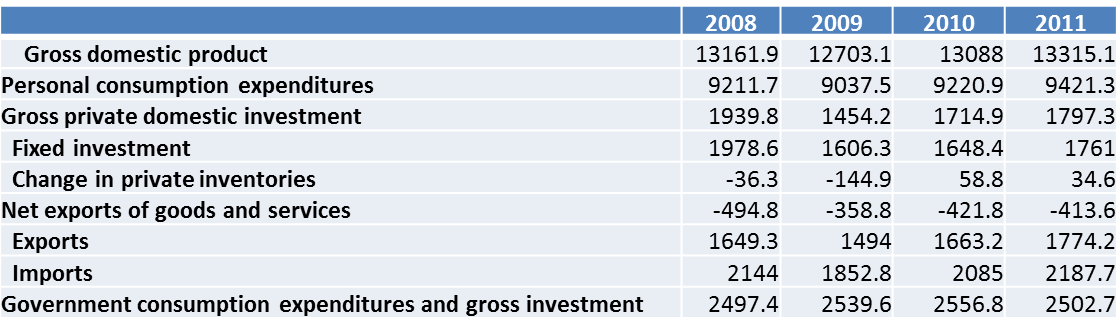
\includegraphics{images/table_2_3.png}

}

\caption{\label{fig-gdp-components}Real GDP and its Components, U.S.A.,
2008--2011, in billions of chained 2005 dollars. Source: Bureau of
Economic Analysis, U.S. Department of Commerce, National Income and
Product Accounts, Table 1.1.6.}

\end{figure}%

\begin{figure}

\centering{

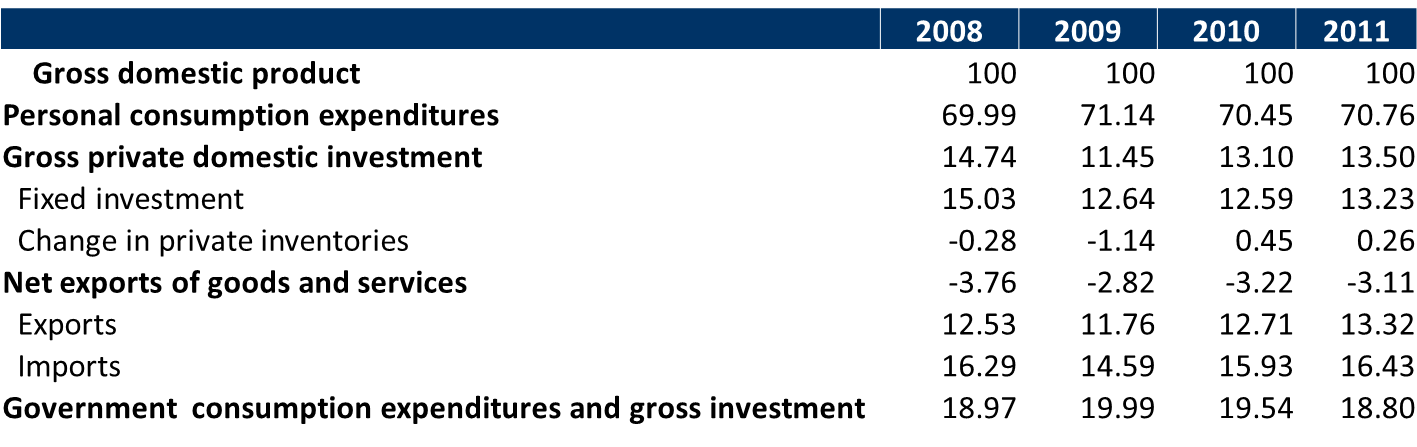
\includegraphics{images/table_2_4.png}

}

\caption{\label{fig-gdp-components-percent}Real GDP and its Components,
U.S.A., 2008--2011, as percent of Real GDP. Source: Bureau of Economic
Analysis, U.S. Department of Commerce, National Income and Product
Accounts, Table 1.1.6.}

\end{figure}%

For my discussion of the theory of international macroeconomics, I will
also use a \emph{forward-looking} definition of the growth rate of a
variable. Specifically, the \textbf{forward-looking growth rate} of
\(x\) is defined as follows:
\begin{equation}\phantomsection\label{eq-f-growthrate}{
x_g\equiv\frac{x_f-x}{x}.
}\end{equation}

Here, \(x_f\) represents the value of \(x\) in the future. Therefore,
\(x_f-x\) represents the increase in the value of \(x\). Therefore,
\((x_f-x)/x\) is the proportionate increase in the value of \(x\) or,
simply, the growth rate of \(x\).

\section{The Components of GDP}\label{sec-gdp-components}

Now that we have discussed the measurement of a country's total
production, let us look at what happens to it. Government statisticians
typically publish data not only on a country's output of final goods and
services (that is, its GDP) but also on who bought those final goods and
services. As in Figure~\ref{fig-gdp-components}, national income data
usually breaks down the big GDP number into four smaller numbers that
represent the final-goods purchases made by four major categories of
buyers:

\begin{itemize}
\tightlist
\item
  personal consumption expenditures (\(C\)),
\item
  gross private domestic investment (\(I\)),
\item
  government purchases (\(G\)), and
\item
  net exports of goods and services (\(NX\)).
\end{itemize}

In other words, Equation~\ref{eq-gdp1}, which is called the national
income identity and breaks down \emph{nominal} gross domestic product
into its components, is equally true for \emph{real} gross domestic
product: \begin{equation}\phantomsection\label{eq-nii}{
Y=C+I+G+NX.
}\end{equation}

\subsection{Consumption}\label{sec-consumption-nia}

\index{consumption!personal consumption expenditures}

The real (i.e., inflation-adjusted) \textbf{personal consumption
expenditures} of the residents of a country in a given year is denoted
by the symbol \(C\). In U.S. data, \(C\) consists of \emph{spending by
households} on all final goods except newly built homes. As you can see
from the U.S. data in Figure~\ref{fig-gdp-components-percent}, \(C\) is
a very large part---more than two-thirds---of GDP.

\subsection{Investment}\label{sec-investment-nia}

\index{investment!gross private domestic investment}

The real \textbf{gross private domestic investment} (or, simply,
investment) of a country is denoted by the symbol \(I\). In U.S. data,
\(I\) consists of:

\begin{itemize}
\tightlist
\item
  the purchases of fixed assets (equipment, software, and buildings) by
  businesses for use in production,
\item
  the purchases of new homes by households,\footnote{As we saw in the
    previous paragraph, this is the only category of household spending
    that is \emph{not} included in \(C\).} and
\item
  increases in inventories of unsold goods held by businesses.
\end{itemize}

Note that the inclusion of these three categories of final goods under
investment is not random. There is an underlying theme here: machines,
new buildings, stocks of as-yet-unsold goods, etc., all contribute to
our \emph{future} welfare.\footnote{The first two categories---fixed
  assets and new homes---are combined into the \emph{fixed investment}
  category in Figure~\ref{fig-gdp-components}.} The money we spend on
pizzas and backrubs, by contrast, are all about the here and now and are
included under consumption, \(C\).

As you can see from the U.S. data in
Figure~\ref{fig-gdp-components-percent}, \(I\), at less than 15\% of
GDP, is a lot less important than \(C\). And yet, because of its
tendency to fluctuate wildly, investment spending is an important cause
of the ups and downs of the overall economy.

\subsubsection{Inventories}\label{sec-inventories}

\index{investment!inventories}

The inclusion of increases in businesses' stocks of unsold goods in
\(I\) needs some justification. What's the point of including this in
\(I\)?

Keep in mind that to get an accurate picture of the health of an economy
in a given year we need to count the market value of all goods and
services produced during the year, whether or not they are sold by
December 31st of that year. Those unsold goods would not be counted in
\(C\), \(I\), \(G\), and \(NX\), if these four variables included only
the actual \emph{purchases} of final goods by households, businesses,
the government, and foreign buyers. To make sure that all goods produced
in 2008 get counted in that year's GDP---even if they are not sold in
2008---statisticians include the additions of unsold goods to
businesses' inventories (or, warehouse stocks) in \(I\).

Note that I did not say that additions to businesses' inventories of
unsold \emph{final} goods are included in \(I\); even the intermediate
goods that were produced in 2008 but not sold by the end of that year
need to be counted in that year's GDP.

Sure, as the ice cream made by Ben \& Jerry's is counted in GDP, one
should not separately count the milk that went into it because the
monetary market value of the ice cream already includes the monetary
market value of the milk. But let's complicate the story a little.
Suppose Ben \& Jerry's buys \$10 million of freshly produced milk some
time in 2008, but does not turn it into ice cream by December 31, 2008.
Instead, the milk is sitting in their freezer on that last day of 2008,
waiting to be turned into Cherry Garcia some time in 2009. This \$10
million worth of milk was produced in 2008 and, therefore, should be
included in 2008's GDP. To ensure this, the rules of GDP accounting
require that any goods that have been added to the inventories (or,
warehouse stocks of goods) of private businesses during 2008 are
\emph{final} goods and their value must be counted in the GDP for 2008.

\subsection{Government Spending}\label{sec-government-spending-nia}

\index{government spending}

Real \textbf{government expenditures} (\(G\)) is pretty much what it
sounds like; it is the inflation-adjusted monetary value of all final
goods and services bought by government entities.

Typically, governments also spend huge amounts of money on
\textbf{transfer payments} or, loosely speaking, gifts (usually to needy
people). But \(G\) includes only the money spent on the purchase of
final goods and does not include transfer payments.

\subsection{Net Exports}\label{sec-netexports-nia}

\index{net exports}

Real \textbf{exports of goods and services} (\(EX\)) is the
inflation-adjusted value of all domestically produced goods that are
bought by foreigners.\index{exports}

Real \textbf{imports of goods and services} (\(IM\)) is the
inflation-adjusted value of all foreign-made goods that are bought by
domestic residents.\index{imports}

Real \textbf{net exports} (\(NX\)) is then defined as
\(NX\equiv EX-IM\). This also goes by other names, such as \textbf{trade
surplus}, \textbf{balance on goods and services}, and, somewhat loosely,
\textbf{balance on the current account}---see
Equation~\ref{eq-balancedef}.\index{trade surplus}\index{current account!balance}
Note, therefore, that \(NX\) could be positive, zero or negative. When
\(NX\) is positive/zero/negative, the country is said to have a
\textbf{Trade Surplus/Balanced Trade/a Trade Deficit}.

\subsubsection{All exports and imports are
final!}\label{sec-exp-imp-final}

There's one more loose end in my definition of GDP that I need to tie
up. Note that in Section~\ref{sec-netexports-nia} above I defined
exports as ``all domestically produced goods that are bought by
foreigners'', not all domestically produced \emph{final} goods''.
Similarly, note that I defined imports as ``all foreign-made goods that
are bought by domestic residents'', not all foreign-made \emph{final}
goods''. Why am I including exports and imports of intermediate goods?
Suppose that American dairy farmers produce \$10 million of milk in 2008
and sell it to a Canadian ice cream company that turns the milk into ice
cream in its plant in Vancouver, also in 2008. The monetary value of the
ice cream would not be counted in America's GDP because the ice cream
was made in Canada. So, if the \$10 million of milk is regarded as an
intermediate good, it would not be counted at all in America's GDP. When
the milk is turned into ice cream by Ben \& Jerry's, the ice cream is
counted in America's GDP and, therefore, so is the milk, although
indirectly. But as for the milk that is sold to a Canadian ice cream
company, the only way to have it counted in America's GDP is to require
that \emph{anything} sold to foreigners is counted in \(EX\). Similarly,
it is straightforward to show that imports of intermediate goods should
be counted in the importing country's \(IM\).

So, here's the final corrected version---fingers crossed!---of the
definition of gross domestic product: \emph{GDP is the monetary market
value of all final goods and services produced within a country in a
given year plus the increase in its inventories of intermediate goods
plus its net exports of intermediate goods}.

\section{The National Income Identity}\label{sec-ni-identity}

To recap, we have so far defined real gross domestic product (\(Y\)),
real personal consumption expenditure (\(C\)), real gross private
domestic investment (\(I\)), real government spending (\(G\)), and real
exports (\(EX\)). It is tempting to argue that \(Y\) must be equal to
\(C+I+G+EX\). After all, \(Y\) represents all final goods that are
``Made in USA'' and any such good would have to be bought either by
American households (\(C\)), or by American businesses (\(I\)), or by
America's government (\(G\)), or by foreigners (\(EX\)). Therefore,
\(Y\) should be equal to \(C+I+G+EX\), right?

Well, not exactly. Although \(C+I+G\), which incidentally is referred to
as \textbf{gross domestic purchases}\index{gross domestic purchases},
does represent the total purchases by domestic households, businesses,
and government entities, it includes purchases of imported goods as well
as domestically produced goods. Therefore, only if we subtract the
inflation-adjusted monetary value of all imported goods (denoted by the
symbol \(IM\)) from \(C+I+G+EX\) would we get \(Y\). That is,
\(Y=C+I+G+EX-IM\).

As we saw in Section~\ref{sec-netexports-nia}, the terms \textbf{net
exports}, \textbf{trade surplus}, and \textbf{balance on goods and
services} all refer to \(NX\equiv EX-IM\), the excess of exports over
imports. Therefore, we get the \textbf{national income
identity}\index{national income identity}:
\begin{equation}\phantomsection\label{eq-ni-identity}{
Y=C+I+G+NX.
}\end{equation}

This is a reappearance of Equation~\ref{eq-gdp1} and
Equation~\ref{eq-nii}.

Figure~\ref{fig-gdp-components} shows data on real gross domestic
product and its components for the United States for the years 2005--8.
You can check that \(C+I+G+NX\) is indeed equal to real GDP.

A theoretically equivalent measure is \textbf{gross domestic income}.
When government statisticians measure the total value added by domestic
producers, they measure the gross domestic product (GDP). When they
measure the total income of all resources employed by domestic
producers, they measure gross domestic income (GDI). As we have seen
above, if measured with perfect accuracy, these two magnitudes should be
the same, as they are theoretically equivalent. In practice, however,
errors do creep in, and the GDP and GDI numbers tend to differ. This
difference is called the \textbf{statistical discrepancy}:
\(GDP=GDI+\text{statistical discrepancy}\).

\subsection{Beyond GDP: Other Measures of Total
Production}\label{sec-beyond-gdp}

Gross domestic product is not the only measure of a country's total
production, there are others.

\subsubsection{Gross National Product}\label{sec-gnp}

\index{gross national product}

Recall that a country's gross domestic product is not only the total
value added by all producers located within the country, it is also
equal to gross domestic income, which is the total income earned by the
factors of production (or, in plain language, resources) employed by all
producers located within the country.\footnote{In other words, if
  measured accurately, GDP \(=\) GDI.}

Some of the resources employed by producers located within the country
may be owned by foreign residents, and the income paid to these
resources goes, necessarily, to their foreign owners. Conversely, some
residents of the domestic country may earn income for work done for
producers located in foreign countries. A country's \textbf{net factor
income earned from foreign residents} (\(NIF\)) \emph{equals} total
income earned by domestic residents from foreign residents \emph{minus}
total income paid by domestic residents to foreign residents.

As, in some cases, it is important to know the total income earned by
the factors of production owned by a country's residents, we often pay
attention to a country's gross national product (GNP):
\begin{equation}\phantomsection\label{eq-gnp}{
\text{GNP}=\text{GDP}+\text{NIF}.
}\end{equation}

A theoretically equivalent measure is gross national income:
\(GNI=GDI+NIF\). Recall from Section~\ref{sec-ni-identity} that although
GDP and GDI are theoretically the same, and would be equal if accurately
measure, in practice the measured magnitudes differ slightly:
\(GDP=GDI+\text{statistical discrepancy}\). The same distinction needs
to be made between GNP and GNI as well; they'd be equal if measured
accurately, but in practice \(GNP=GNI+\text{statistical discrepancy}\).

\subsubsection{Gross National Disposable Income}\label{sec-gndi}

\index{gross national disposable income}

The residents of a country may send gifts to---and receive gifts
from---the residents of other countries. A country's \textbf{net
unilateral transfers of income from foreign residents} (NUT) is defined
as gifts received \emph{minus} gifts given. Gross national disposable
income (GNDI) is then defined as
\begin{equation}\phantomsection\label{eq-gndi}{
\text{GNDI}=\text{GNI}+\text{NUT}.
}\end{equation}

Recall that gross domestic product is denoted by the symbol \(Y\). In
practice, the statistical discrepancy between GDP and GDI (or between
GNP and GNI) is small. Moreover, net factor income earned from foreign
residents (NIF) and net unilateral transfers of income from foreign
residents (NUT) tend to be small too. As a result, the differences
between GDP, GDI, GNP, GNI, and GNDI are, for most practical purposes,
small enough to be ignored. Consequently, to keep the discussion simple,
I will use the symbol \(Y\) to refer to \emph{all} these different ways
of measuring a country's total value added, total income, and total
expenditure.

\subsubsection{National Income Identity, Revisited}\label{sec-nii-2}

\index{national income identity}

Recall from Equation~\ref{eq-ni-identity} that \[ Y=C+I+G+NX.\]
Therefore, \[Y+\text{NIF}+\text{NUT}=C+I+G+NX+\text{NIF}+\text{NUT}.\]
It is clear from equations Equation~\ref{eq-gnp} and
Equation~\ref{eq-gndi}, the last equation can be re-written as \[
\text{GNDI}=C+I+G+(NX+\text{NIF}+\text{NUT}). 
\]

As we will see in the next chapter's discussion of balance of payments
accounting, the expression within parentheses in the last equation is
called the \textbf{balance on the current account} or, simply the
current account (CA). The equation above then yields a slightly updated
version of the national income identity:
\begin{equation}\phantomsection\label{eq-nii-ca}{
\text{GNDI}=C+I+G+CA.
}\end{equation}

The reader should be warned, however, that I will use the terms net
exports (\(NX\)) and current account balance (\(CA=NX+NIF+NUT\))
interchangeably throughout this book, because---as was pointed out a
short while back in Section~\ref{sec-gndi}---both \(NIF\) and \(NUT\)
tend to be small in magnitude.

\section{Prices and Inflation}\label{sec-p-pi}

Inflation is a topic of major concern in economics as well as in our
daily lives. Therefore, it is important to understand what causes it and
how it can be controlled. But before we can get to that, we need to
discuss how inflation is measured.

The measurement of inflation can be quite tricky. While the prices of
some goods may rise from one year to the next, the prices of other goods
may fall. In such cases, one needs to come up with \emph{one} number
that summarizes the \emph{overall} change in prices.

\subsection{The Implicit Price Deflator for GDP}\label{sec-IPDGDP}

\index{gross domestic product!implicit price deflator for}

Suppose you recently spent a day in Boston followed by a day in San
Antonio. You ate the same meals in both cities, bought the same
newspaper, rented the same type of car, and stayed in identical hotels.
Nevertheless, you ended up spending 10\% more in Boston. Why? You did
not buy more stuff in Boston; in fact, you bought exactly the same
things in both cities. Therefore, the only explanation is that prices
were higher overall in Boston. Some things may be cheaper in Boston and
some other things may be cheaper in San Antonio. But it is reasonable to
conclude---from your own limited experience in the two cities---that the
overall level of prices was 10\% higher in Boston relative to San
Antonio.

Now consider another hypothetical example. Suppose you spent both
October 1, 2005 and October 1, 2006 in Boston and during both visits you
bought the exact same things, used the same transportation, and stayed
in identical hotel rooms. And yet, you ended up spending 4\% more in
2006 than in 2005. Using the same logic as in the last paragraph, we can
conclude that although individual items' prices may have changed at
different rates, the overall level of prices in Boston rose 4\% in 2006
relative to 2005.

In fact, you don't even have to visit Boston on two different dates.
After your October 1, 2006 visit, you could dig up data on the prices
that you would have paid if you had visited Boston a year earlier and
bought the same goods and services that you bought during your October
1, 2006 visit, and you would have again reached the conclusion that the
overall level of prices rose 4\% in Boston in 2006. And that, by and
large, is what government statisticians do to measure the rates of
change of the overall level of prices in the US and other countries.

One way to measure the overall level of prices is to compare the nominal
GDP and the real GDP for a particular year. We see in
Table~\ref{tbl-gdp-n-deflator} that in 1999 America's nominal GDP was
\$9,353.5 billion and America's real GDP, with base year 2005, was
\$10,779.8 billion. Stated differently, in 1999 America's nominal GDP
was 86.8\% of America's real GDP: \[
\begin{eqnarray*} 
\frac{\text{Nominal GDP in 1999}}{\text{Real GDP in 1999 with base year 2005}}\times 100&=&\frac{9,353.5}{10,779.8}\times 100\\
&=& 86.8.
\end{eqnarray*} 
\] So, at 1999 prices, the dollar value of all final goods produced in
the U.S. in 1999 was \$9,353.5 billion, whereas, at 2005 prices, the
dollar value of the exact same goods was \$10,779.8 billion.

Now, how could one dollar value of the final goods made in 1999 be
different from the other dollar value of the exact same goods? As the
quantities used in the nominal GDP calculation are the same as the
quantities used in the real GDP calculation, these two dollar values
must be different because they use different \emph{prices}.

More precisely, the only possible reason why America's nominal GDP in
1999 is 86.8\% of America's real GDP in 1999 must be that the prices
that prevailed in 1999, which are the ones that were used in the
calculation of nominal GDP, were, in an overall sense, 86.8\% as high as
the prices that had prevailed in 2005, which are the ones that were used
in the calculation of real GDP.

It would be incorrect to conclude that \emph{all} final goods were
86.8\% as pricey in 1999 as in 2005. For apples, the 1999 price may have
been 80\% of the 2005 price. For haircuts, the 1999 price may have been
130\% of the 2005 price. For gas at the pump, the 1999 price may have
been 99\% of the 2005 price. But it is reasonable to say that in an
overall sense the 1999 prices were 86.8\% as high as the 2005 prices
because the final goods that were produced in America in 1999 were only
86.8\% as valuable at 1999 prices than at 2005 prices.

Thus, by comparing the nominal and real GDP values for a particular year
we are able to measure how that year's prices as a whole measure up
relative to the base year's prices. Formally, the

\begin{equation}\phantomsection\label{eq-IPDGDP}{
\text{Implicit Price Deflator for GDP in year $n$ with base year $m$} = \frac{\text{Nominal GDP in year $n$}}{\text{Real GDP in year $n$ with base year $m$}}\times 100
}\end{equation} shows what the overall level of final goods' prices in
year \(n\) was as a percentage of the base year's overall price level.
More compactly,
\begin{equation}\phantomsection\label{eq-IPDGDP_compact}{ 
\text{Implicit Price Deflator}=
\frac{\text{Nominal GDP}}{\text{Real GDP}}\times 100.
}\end{equation}

The fourth column in Table~\ref{tbl-gdp-n-deflator} shows America's
implicit price deflator for GDP (IPDGDP) for the 1999--2008 decade.
Specifically, it shows that the overall level of prices in 1999 was
86.8\% of the overall level of prices in 2005. Similarly, the overall
level of prices in 2005 was 100\% of the overall level of prices in
2005---what a shocker!---and the overall price level in 2007 was 106.2\%
of the overall level of prices in 2005.\footnote{If you saw
  Table~\ref{tbl-gdp-n-deflator}, but without any information about 2005
  being the base year in the heading of the third column, would you
  still be able to figure out that 2005 is the base year?}

In the remainder of these lectures, I will represent the overall price
level for a particular year not by the implicit price deflator for GDP
but by a very slightly different version of it:
\begin{equation}\phantomsection\label{eq-P}{
\begin{eqnarray}
P&=&\frac{\text{Implicit Price Deflator for GDP}}{100}\nonumber \\
&=&\frac{\text{Nominal GDP}}{\text{Real GDP}}\times\frac{100}{100}\nonumber \\
&=&\frac{\text{Nominal GDP}}{Y}.
\end{eqnarray}
}\end{equation} Note that Equation~\ref{eq-P} comes from equation
Equation~\ref{eq-IPDGDP}.

In other words, while real GDP is represented by the symbol \(Y\), the
overall level of prices is denoted by the symbol \(P\), and nominal GDP
is given by \begin{equation}\phantomsection\label{eq-nomGDP}{
\text{Nominal GDP}=P\times Y.
}\end{equation}

\subsection{The Consumer Price Index}\label{sec-cpi}

\index{consumer price index}

The implicit price deflator for GDP is not the only one-number
representation of the overall level of the prices of the innumerable
goods that are bought and sold in a modern economy. Indeed, it may not
even be the most popular method: a frequently cited alternative measure
of the overall level of prices is the \textbf{consumer price index}.

Whereas the implicit price deflator for GDP is (100 times) the value of
the current year's output of final goods at the current year's prices
divided by the value of the same set of goods at the base year's prices,
the consumer price index is (100 times) the value of \emph{a fixed
bundle of goods that represents the purchases of a }typical consumer* at
the current year's prices divided by the value of that same bundle of
goods at the base year's prices.

Although Equation~\ref{eq-P} sees the overall price level, \(P\), as the
implicit deflator for GDP divided by 100, you may, if you wish, think of
\(P\) as the consumer price index divided by 100. In practical terms,
these two measures of the overall price level tend to move in sync most
of the time.\footnote{However, an increase in the price of M16 rifles,
  which are usually bought by a country's armed forces but not by its
  typical consumer---not yet anyway!---would raise the value of the GDP
  deflator but not the CPI.}

\subsection{Inflation}\label{sec-inflation}

\index{inflation!measurement}

Finally, how do we measure inflation? Inflation is defined simply as the
growth rate of the overall level of prices, where the term `growth rate'
is as it is defined in Section~\ref{sec-notngrowth}. I will denote
inflation by the symbol \(\pi\), which is the lower-case Greek letter
`pi'. Denoting the past value of the overall price level by the symbol
\(P_{-1}\), we can use equation Equation~\ref{eq-growthrate} to express
inflation as follows:
\begin{equation}\phantomsection\label{eq-inflation}{
\pi\equiv\frac{P-P_{-1}}{P_{-1}}\equiv\frac{P}{P_{-1}}-1.
}\end{equation} The increase in the overall price level is \(P-P_{-1}\).
But the proportionate increase in \(P\) is \((P-P_{-1})/P_{-1}\). And to
express inflation as a \emph{percentage}, one has to multiply \(\pi\) by
100.

For example, the annual inflation rate for, say, 2004 is
\begin{equation}\phantomsection\label{eq-inflation2004}{
\begin{eqnarray} 
{\text{Inflation during 2004}}\nonumber \\
&=&\frac{P_{2004}-P_{2003}}{P_{2003}}\times 100\\
&=&\frac{\text{IPDGDP}_{2004}-\text{IPDGDP}_{2003}}{\text{IPDGDP}_{2003}}\times 100\\
&=&\frac{96.77-94.1}{94.1}\times 100\nonumber \\
&=&2.8 \text{ percent}.\nonumber 
\end{eqnarray}
}\end{equation}

America's annual inflation rates, as defined above, are shown in
Table~\ref{tbl-growth-inflation} for 1999--2008. Although these
inflation numbers are calculated based on the implicit price deflator
for GDP as the price level, one could also think of inflation as the
annual percentage increase in the consumer price index, which has been
discussed above in Section~\ref{sec-cpi}. In practical terms, this does
not make much difference to inflation data, especially over longer
periods, as you can see in Figure~\ref{fig-inflation}. Over short
periods of time, however, inflation measures based on the consumer price
index are more volatile, as can be seen in
Figure~\ref{fig-cpi-volatile}\}.

\begin{figure}

\centering{

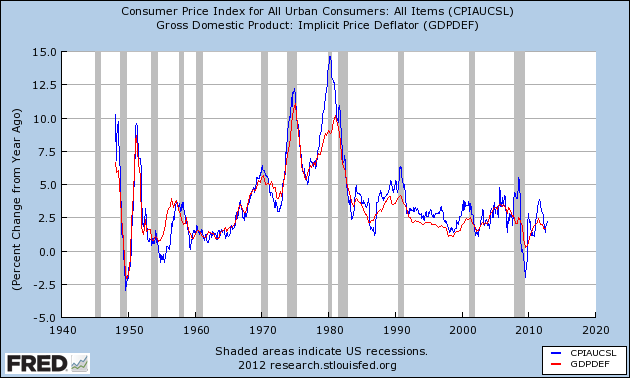
\includegraphics{images/cpiaucsl-gdpdef-fredgraph.png}

}

\caption{\label{fig-inflation}Inflation: Two Measures The red graph
represents US inflation measured by the year-on-year percentage change
in the implicit price deflator for GDP. The blue graph uses the consumer
price index (for all urban consumers) instead. Source: Data on the
implicit price deflator for GDP was downloaded from
\url{http://research.stlouisfed.org/fred2/series/GDPDEF} and data on the
consumer price index was downloaded from
\url{http://research.stlouisfed.org/fred2/series/CPIAUCSL}, both on
November 25, 2012.}

\end{figure}%

\begin{figure}

\centering{

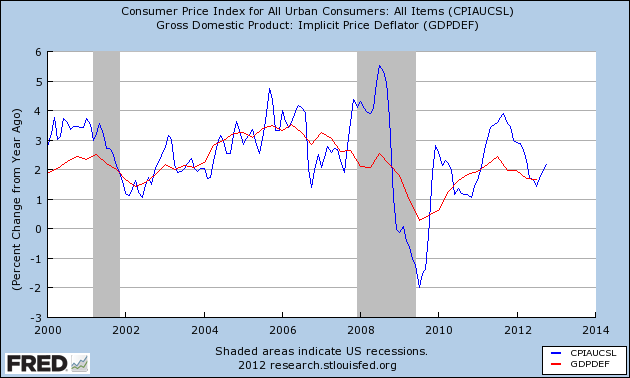
\includegraphics{images/cpiaucsl-gdpdef-fredgraph-b.png}

}

\caption{\label{fig-cpi-volatile}\textbf{Inflation: CPI Is More
Volatile} The red graph represents US inflation measured by the
year-on-year percentage change in the implicit price deflator for GDP.
The blue graph uses the consumer price index (for all urban consumers)
instead. This chart focuses on the 21st century and highlights the
volatility of the CPI. Source: Data on the implicit price deflator for
GDP was downloaded from
\url{http://research.stlouisfed.org/fred2/series/GDPDEF} and data on the
consumer price index was downloaded from
\url{http://research.stlouisfed.org/fred2/series/CPIAUCSL}, both on
November 25, 2012.}

\end{figure}%

\bookmarksetup{startatroot}

\chapter{Balance of Payments Accounts}\label{sec-bopacc}

A country's balance of payments\index{balance of payments} account for,
say, 2003 summarizes all economic transactions that took place between
its residents and foreign residents during 2003.

The balance of payments accounts consist of the \textbf{current
account}, the \textbf{capital account}, and the \textbf{financial
account}.

\section{The Current Account}\label{sec-curacc}

To keep things simple, let's assume that in every transaction there is
one person who hands over some goods, services or assets and another
person who pays (for those goods, services or assets) with
cash.\footnote{By assets I mean \emph{non-cash} assets. It is possible
  that a US resident might buy some Swedish kroner, which is a cash
  asset, and just hang on to it. But I will keep things simple by
  assuming that a US resident who buys some Swedish kroner would
  immediately spend it on some goods, services or non-cash assets (such
  as stocks, bonds, the title to a house, etc.) perhaps because she has
  no use for Swedish kroner in the US. As a result, it makes sense to
  assume that when cash is offered as payment, it is to buy some
  non-cash asset. Moreover, although it is possible for Alan to hand
  over some IBM shares to Betty and get some Google shares in return,
  not much realism is lost by assuming that Alan gets cash for his IBM
  shares and then uses the cash to buy Google shares from Betty.}

Transactions in which \emph{goods or services} are traded between
\emph{residents} of America and \emph{residents} of other countries are
summarized in America's current
account\index{balance of payments!current account}.

\section{The Capital Account}\label{sec-capacc}

The balance of payments accounts also includes the capital
account\index{balance of payments!capital account}. But I will ignore it
because it usually involves small sums of money and is not important for
my purposes. According to \textcite{gerber2002}, page 176, ``The capital
account includes transfers of specific types of capital, such as debt
forgiveness, the personal assets that migrants take with them when they
cross international boundaries, and the transfer of real estate and
other fixed assets, such as the transfer of ownership of a military base
or an embassy.''

Prior to 1996 what we now call the financial account used to be called
the capital account and used to include what we now call the capital
account.

To repeat, I will ignore the capital account. That is, unless I make an
explicit statement to the contrary, I will assume that none of the types
of international transactions that are formally classified under the
capital account are actually taking place.

\section{The Financial Account}\label{sec-finacc}

Transactions in which \emph{assets} are traded between residents of
America and residents of other countries are summarized in America's
financial account\index{balance of payments!financial account}.

An \textbf{asset}\index{asset} is pretty much anything that you can buy
today (if you have some surplus cash) and sell later (if you need some
extra cash). If your asset provides some service to someone while you
are its owner, you can earn an \emph{income} from your asset. For
example, if an American buys a house in Germany, she would be buying an
\emph{asset}. And the rental income she earns by renting out the house
is her \emph{asset income}. If an American buys a German company's
stock, she would be buying an \emph{asset}. And the dividend income she
earns (as long as she owns the stock) is her \emph{asset income}. If an
American puts money in a German bank, that bank account is an
\emph{asset} that will periodically yield interest \emph{income}.

Interestingly, while \emph{international asset trades are recorded in
the financial account} of a nation's balance of payments, the
\emph{income earned from those assets are considered to be payments for
services rendered by the assets and are, therefore, recorded in the
current account}. So, an American's purchase of a house in Germany will
be recorded in the financial account and any subsequent rental income
from that house will be recorded in the current account.

The financial account includes the \textbf{Official Reserve Transactions
Account}\index{balance of payments!financial account!Official Reserve Transactions Account}.
Most countries have \textbf{central banks}\index{central banks} that
design and carry out their monetary policies. For example, America's
central bank is the Federal Reserve (or, simply, the
Fed\index{central banks!Fed, the}). Central banks often buy and/or sell
assets. For example, the Bank of
Japan\index{central banks!Japan, Bank of} (i.e., Japan's central bank)
may buy U.S. Treasury bonds. It may then sell those bonds at a later
date if it needs dollars. The assets that central banks typically buy
and sell are called \textbf{reserve assets}\index{reserve assets}.
\emph{International trade in reserve assets conducted by central banks
is recorded in the official reserve transactions account}.

\section{Credits, Debits, and
Balances}\label{sec-credits-debits-balances}

Recall that all economic transactions that take place between a
country's residents and the residents of other countries are recorded in
the country's current, capital, and financial accounts. The recording of
these transactions follows strict rules. This section presents a
simplified look at the rules of balance of payments accounting.

\subsection{Which Transactions Are Recorded as
Credits?}\label{sec-credits}

Recall from Section~\ref{sec-curacc} that I have assumed that in every
transaction there is one person who hands over goods, services or
non-cash assets (such as stocks and bonds) and another person who pays
with cash or check (i.e., money; to economists, both currency and checks
count as money). Any transaction resulting in a receipt of money from
foreigners is entered in the balance of payments accounts as a
credit\index{balance of payments!credits} and is given a positive
(\(+\)) sign. In other words, any transaction in which we sell (i.e.,
\emph{export}) goods, services or assets to foreigners is recorded as a
\emph{credit}.

\subsection{Which Transactions Are Recorded as
Debits?}\label{sec-debits}

Any transaction in which we pay money to foreigners is entered in the
balance of payments accounts as a
debit\index{balance of payments!debits} and is given a negative (\(-\))
sign. In other words, \emph{imports} of goods, services and assets are
recorded as \emph{debits}.

\section{Accounting Rules: Examples}\label{sec-accex}

Here are some examples that illustrate the rules of balance of payments
accounting that I have discussed above:

\begin{itemize}
\tightlist
\item
  The sale (i.e., export) of a U.S. car to Germany is a \emph{credit} in
  the U.S. \emph{current} account.
\item
  An American's purchase (i.e., import) of a house in Germany is a
  \emph{debit} in America's \emph{capital} account.
\item
  The rental income earned by an American from her house in Germany is
  seen as the \emph{export} of housing services from America to Germany
  and is, therefore, a \emph{credit} in America's \emph{current}
  account.
\item
  When a German deposits some extra cash in his New York bank account,
  it is seen as the purchase by the German (and, therefore, an
  \emph{export} by America) of an American asset (in this case, the
  increased value of the bank account) and is recorded as a
  \emph{credit} in America's \emph{financial} account.
\end{itemize}

Note again that \emph{credits are always exports} of goods, services or
assets and \emph{debits are always imports}.

\subsection{\texorpdfstring{What Is the \emph{Balance} on an
Account?}{What Is the Balance on an Account?}}\label{sec-balance}

\emph{The total of all credits minus the total of all debits in an
account or sub-account is called its
balance}\index{balance of payments!balance}. The balance could be
positive, zero, or negative.

Since credits are exports and debits are imports,
\begin{equation}\phantomsection\label{eq-balancedef}{
\text{Balance} = \text{Credits} - \text{Debits} = \text{Exports} - \text{Imports} = \text{Net Exports}.
}\end{equation} In particular, \emph{our current account balance is our
net export of goods and services} and \emph{our financial account
balance is our net export of assets}.

Most internationally traded assets are paper assets such as stocks and
bonds. Unlike the purchase of, say, a house, the purchase of a stock or
a bond does not involve the exchange of some tangible commodity. The
purchase of stocks and bonds simply entitle the buyer to future income.
If you buy Microsoft stock, Microsoft will get your money \emph{today}
and you will receive a share of Microsoft's \emph{future} profits (as
long as you keep the stock). If you buy a bond from AT\&T, AT\&T will
get your money \emph{today} and you will get regular \emph{future}
payments of some amount specified on the bond. Notice that in both of
these last two cases, what you are really doing is \emph{lending} some
of your money to others \emph{today} in the expectation that they will
pay you in the \emph{future}. When you buy Microsoft stock, you are
lending money to Microsoft. When you buy AT\&T bonds, you are lending
money to AT\&T. Similarly, the sale of stocks (by, say, Microsoft) and
bonds (by, say, AT\&T) is simply a way for these companies to borrow
money.

Applying this idea to international asset trades, \emph{America's sale
(or, export) of stocks and bonds to foreigners during 1999 is equal to
the amount America borrowed from foreigners during 1999 and America's
purchase (or, import) of stocks and bonds from foreigners during 1999 is
equal to the amount America loaned to foreigners during 1999. Therefore,
our financial account balance for 1999 is equal to the increase in our
net indebtedness to foreigners during 1999}.

\begin{equation}\phantomsection\label{eq-intdebt}{
\begin{eqnarray}
{\text{Financial Account Balance in 1999}}\\
&=&\text{Financial Account Credits}-\text{Financial Account Debits}\nonumber\\
&=&\text{Assets Exports}-\text{Assets Imports}\nonumber\\
&=&\text{Borrowing from foreigners in 1999}-\text{Lending to foreigners in 1999}\nonumber\\
&=&\text{Increase in our net indebtedness in 1999.}\nonumber
\end{eqnarray}
}\end{equation}

If, for example, our financial account balance during 1999 was +\$100
billion, then we borrowed \$100 billion more from foreigners than we
lent them, and, so, our indebtedness to foreigners increased in 1999 by
\$100 billion.

And, by the way, that increase of \$100 billion in our foreign debt
could have happened in several different ways: For example, the amount
we owe them could have gone up from \$500 billion to \$600 billion or
the amount they owe us could have gone down from \$300 billion to \$200
billion or their debt to us of \$25 billion may have turned into our
debt to them of \$75 billion during 1999.

If, on the other hand, our financial account balance was -\$150 billion,
then our net indebtedness to foreigners decreased by \$150 billion.
\emph{Therefore, a positive financial account balance means an increase
in our international indebtedness and a negative financial account
balance means a decrease in our international indebtedness}.

\section{Balance of Payments Identity}\label{sec-curcap}

Now that we have seen how the balances in the current, capital, and
financial accounts are defined, it is necessary to see how the three
balances are related. It turns out that \emph{the balances of the
current, capital, and financial accounts must always sum to zero}:

\begin{equation}\phantomsection\label{eq-balancedpayments}{
\text{current account balance} + \text{capital account balance} + \text{financial account balance} \equiv 0.
}\end{equation}

So, if we ignore the typically tiny capital account, if the current
account balance is \(-\)\$5000, then the financial account balance would
have to be +\$5000, and vice versa.

To see the logic behind Equation~\ref{eq-balancedpayments}, let the
current account balance be \(-\)\$5000. In other words, our net export
of goods and services is \(-\)\$5000. That is, we bought \$5000 more
goods and services from foreigners than we sold to them. This raises a
question: How could it have happened? Are we living on the charity of
foreigners? Why would they give us \$5000 more stuff than we gave them?
The answer is that the foreigners will let us have an additional \$5000
worth of \emph{goods and services} as long as we give them an additional
\$5000 of \emph{assets}. That is, our net export of goods and services
may be \(-\)\$5000 as long as our net export of assets is \(+\)\$5000.
Therefore, recalling from Equation~\ref{eq-balancedef} that ``net
export'' is also called ``balance'', our current account balance can be
\(-\)\$5000 as long as our financial account balance is \(+\)\$5000.

We saw in Section~\ref{sec-balance} that a positive financial account
balance reflects an increase in our net indebtedness to foreigners.
Therefore, Equation~\ref{eq-balancedpayments} means that we can import
more goods and services than we export, as long as we understand that
there will be an increase in our net indebtedness.

Another way to see this is to recognize that every international
transaction will necessarily involve a credit in one of the two
accounts---i.e., in either the current account or the financial
account---and a debit of equal size in the other account.

Consider an example. Suppose a German buys an American car for \$50,000.
This is a credit in the current account and, therefore, our current
account balance increases by \$50,000. Now, where would the German buyer
get those dollars? There are several possibilities:

\begin{itemize}
\tightlist
\item
  He has a bank account in New York from which he pays the \$50,000. In
  this case, following example 4 in Section~\ref{sec-accex} above, we
  can see that this is a debit of \$50,000 in our financial account. So,
  our financial account balance decreases by \$50,000.
\item
  He sells some of his U.S. assets (such as real estate or stocks or
  bonds) and uses that money to buy his car. Again, a glance at examples
  2 and 4 in Section~\ref{sec-accex} will show you that this has the
  same effect as in the previous case: our financial account balance
  decreases by \$50,000.
\item
  He buys \$50,000 from an American who needed Euros to open a bank
  account in Germany. As you can tell from example 4 in
  Section~\ref{sec-accex}, this is a \$50,000 debit in our financial
  account. So, again, our financial account balance decreases by
  \$50,000.
\end{itemize}

The point of these examples is that if a transaction causes our current
account balance to \emph{increase} by \$50,000, then it must
simultaneously involve another transaction that causes our financial
account balance to \emph{decrease} by the same amount, irrespective of
the gory details of the transaction.

Similarly, it can be shown that any transaction that \emph{decreases}
our current account balance by \$40,000 will simultaneously be
accompanied by other transactions that will \emph{increase} our
financial account balance by \$40,000.

More generally, any transaction that changes the balance on any of these
two accounts will be accompanied by other transactions that change the
balance on the other account by the same amount but in the opposite
direction. Hence, the current account balance plus the financial account
balance must always be zero.

In other words---using the idea that the balance on an account is equal
to the net exports on that account; see equation
Equation~\ref{eq-balancedef} --- the net exports of goods and services
must equal the net imports of assets, and vice versa.

\bookmarksetup{startatroot}

\chapter{Exchange Rates}\label{sec-exrates}

The currency of a country is valuable, even to residents of other
countries. Non-Americans may wish to buy dollars (with their own
respective currencies), in order to buy American goods, services or
assets.\footnote{By ``non-Americans'' I mean residents of countries
  other than the United States. Similarly, by ``Americans'' I mean
  residents of the United States, citizens or not.} Similarly, Americans
may be willing to pay dollars to buy foreign currencies. The
institutions that enable people to trade one currency for another are
called \textbf{foreign exchange
markets}\index{markets!foreign exchange}. The amount of currency \(A\)
(say, the US dollar) that will have to be paid as the price of one unit
of currency \(B\) (say, the euro) in the foreign exchange market is the
\textbf{exchange rate}\index{exchange rate} of currency \(B\) in terms
of currency \(A\).

\section{Nominal Exchange Rates}\label{sec-nomexrates}

The answer to the question ``What are \emph{nominal} exchange rates?''
is actually the same as the answer to the question ``What are exchange
rates?''. The nominal exchange
rate\index{exchange rate!nominal exchange rate} of the euro in terms of,
say, the US dollar is the price of a euro in dollars. The word
``nominal'' is sometimes added simply to serve as a reminder that there
exists another kind of exchange rate: the real exchange rate.

In this lecture, I will typically consider two currencies: the
\emph{domestic} currency and the \emph{foreign} currency. I will use the
symbol \(E\) to denote \textbf{the price of the foreign currency
measured in units of the domestic currency}. So, if the domestic
currency is the US dollar and the foreign currency is the British pound,
and if one pound is worth \$2.00, then \(E = 2.00\). If one US dollar is
worth 100 Japanese yen, then \(E=0.01\). (Why?)

\section{Real Exchange Rates}\label{sec-realexrates}

The real exchange rate\index{exchange rate!real exchange rate} is
\emph{the (average) price of foreign-made goods and services measured in
units of domestically produced goods and services}. It is denoted by the
symbol, \(q\), of the lower case Greek letter ``epsilon'', and it is
computed by the following equation:
\begin{equation}\phantomsection\label{eq-q}{
q=\frac{E\cdot P^*}{P}
}\end{equation}

Here, \(P\) (respectively, \(P^*\)) represents \textbf{the average level
of prices} of goods and services made in the domestic (respectively,
foreign) economy. By ``average level of prices'' I mean some sort of
price index such as the implicit price deflator for GDP or the consumer
price index\index{consumer price index}.\footnote{These variables were
  discussed in Section~\ref{sec-p-pi}. See in particular
  Equation~\ref{eq-P}.}

To see why Equation~\ref{eq-q} does measure the relative price of
foreign goods in units of domestic goods, consider a world in which
wheat is the only traded good. Consider ``Made in USA'' wheat and ``Made
in France'' wheat. Let the price of ``Made in USA'' wheat be \$2.00 per
pound; that is, let \(P=2\). Let the price of ``Made in France'' wheat
be \EUR{6.00} per pound; that is, let \(P^*=6\). Let the price of one
euro be \$2.00; that is, let \(E=2.00\). Note that the price of ``Made
in France'' wheat is \EUR{6.00} which is worth \$12.00. Note also that
\$12.00 would buy you six pounds of ``Made in USA'' wheat. Therefore,
one pound of ``Made in France'' wheat has the same market value as six
pounds of ``Made in USA'' wheat. That is, the real exchange rate of
``Made in France'' wheat is six pounds of ``Made in USA'' wheat. In
symbols, \(q=6\).

Let us now see if the formula in Equation~\ref{eq-q} gives the same
answer. If we substitute \(P=2\), \(P^*=6\) and \(E=2.00\) in
Equation~\ref{eq-q}, we get \(q=(2.00\times 6)/2 =6\), which is exactly
the real exchange rate we got in the last paragraph.

Note that the real exchange rate, being the price of foreign-made goods
(measured in units of domestically produced goods), is a measure of the
foreign economy's
competitiveness\index{exchange rate!real exchange rate!competitiveness}.
The higher the value of \(q\), the less attractive foreign-made goods
would be (to domestic buyers) and the more attractive domestically
produced goods would be (to foreign buyers).

\subsection{Notation: Foreign Country Variables}\label{sec-notnfornvar}

As I did in the case of \(P^*\) in Section~\ref{sec-realexrates}, I will
use an asterisk (*) as a superscript to mark all foreign variables;
i.e., all variables describing the rest of the world.

\section{What Are Spot Exchange Rates?}\label{sec-spotexrates}

The spot exchange rate is just another way of refering to the exchange
rate that I discussed earlier in Chapter~\ref{sec-exrates}. Today's spot
exchange rate\index{exchange rate!spot exchange rate} of, say, the
Japanese yen in terms of the US dollar is the price---of a yen, in
dollars---at which any dollar-yen exchange would take place today. This
is, therefore, just another, fancier name for the \(E\) that was defined
earlier. The word ``spot'' is sometimes added simply to serve as a
reminder that there exists another kind of exchange rate: the Forward
Exchange Rate.

\section{What Are Forward Exchange Rates?}\label{sec-forwardexrates}

Today's ``30-day forward exchange
rate''\index{exchange rate!forward exchange rate} of the yen in terms of
the US dollar is the price---of a yen, in dollars---that you would have
to pay for any dollar-yen exchange you agree \emph{today} to do \emph{30
days later}. Only the agreement is signed today; the actual exchange of
currencies takes place 30 days later. Let us denote the 30-day forward
exchange rate of the foreign currency in terms of the domestic currency
by \(f_{30}\). So, if \(f_{30} = 0.095\) US dollars today, you can sign
an agreement today to sell \$9.50 thirty days later in exchange for 100
yen.

But why would anyone do such a thing? That is, why would one sign an
agreement \emph{today} to make a currency exchange \emph{thirty days
later?} Well, by trading currencies on the forward exchange market, one
can \emph{avoid exchange rate uncertainty}. Suppose you will have to pay
someone 100 yen thirty days from today. If you sign a forward-market
agreement today and if \(f_{30}=0.095\), you'll know that you'll need
exactly \$9.50 thirty days later to make your 100 yen payment. You could
instead wait 30 days, go to the foreign exchange spot market and buy 100
yen at whatever spot-market exchange rate prevails at that date. But
that would be a gamble: you could end up paying \$9.50 or more than
\$9.50 or less than \$9.50 depending on what the spot rate is at that
date.

\subsection{Forward Exchange Rates and
Expectations}\label{sec-forward-exp}

It can be shown that the 30-day forward exchange rate of the yen is a
proxy measure of what people currently expect the spot-market value of
the yen will be 30 days in the future. That is, if \(f_{30} = 0.095\) US
dollars per yen today, then it is a safe bet that people today expect
that one yen will be worth \$0.095 thirty days later in the spot market.
Why?

Recall that the nominal exchange rate (\(E\)) is the current spot-market
value of one unit of the foreign currency. Using the notational rule set
out in Section~\ref{sec-notngrowth}, let \(E_f\) denote the
\emph{future} spot-market value of one unit of the foreign currency.
And, finally, let \(E_f^e\) denote the \textbf{current expectation of
the future value of the nominal exchange rate}. My claim is that
\(f_{30}\) is a good estimate of \(E_f^e\) when the future is 30 days
ahead.

To see why this is, suppose, to the contrary, that \(f_{30} = 0.095\) US
dollars per yen today, but that people today think that thirty days
later one yen will be worth \(E_f^e =0.080\) US dollars in the spot
market. Now, if people are more or less convinced that thirty days later
they would be able to buy one yen in the spot market for \$0.080, why
would they rush to the forward market today and pay \$0.095 for every
yen that they must pledge to buy thirty days later? It doesn't make
sense. If instead we had \(f_{30} = 0.095\) and \(E_f^e =0.099\), then
people would indeed want to buy yen in the forward market.

But now nobody would want to \emph{sell} yen in the forward market. To
see why, suppose you are an American exporter and you are expecting a
Japanese client to pay you in yen thirty days in the future. You could
wait till you receive the yen payment and then sell your yen on the spot
market to get dollars, or you could sell the expected receipt of yen on
the forward market \emph{today}. Which would you rather do? As the
forward value of a yen is \(f_{30} = 0.095\) and you expect that the
spot-market value will be \(E_f^e =0.099\), you will surely choose to
avoid the forward market.

To summarize, I have established that if \(f_{30} > E_f^e\) then nobody
would want to buy the foreign currency in the forward market. I have
also established that if \(f_{30} < E_f^e\) then nobody would want to
sell the foreign currency in the forward market. Therefore, the only
reasonable outcome is \(f_{30} = E_f^e\). That is, today's
forward-market price of a currency is a good estimate of what people
today expect that currency's spot-market value will be in the future.

Typically, you can't tell what people expect the future to be. But in
the case of foreign exchange rates at least, there is a way to do so!

\bookmarksetup{startatroot}

\chapter{Markets and Equilibrium}\label{sec-basicequations}

A theory that says ``Anything is possible'' or ``All conceivable
outcomes are equally plausible'' would not be of any use. To be useful,
a theory must put its foot down and take a stand on which outcomes are
plausible and which outcomes are not. For an outcome to be considered
plausible, the typical theory in economics requires that all relevant
markets (for goods, services, and assets) be in equilibrium, which is
when supply and demand are equal. This chapter describes the conditions
that must prevail in the markets for goods, money, and foreign currency
for them to be in equilibrium.

\section{The Goods Market Equilibrium Condition}\label{sec-goodseqm}

\index{equilibrium!goods market}

The goods market\index{markets!goods} is said to be in equilibrium when

\begin{equation}\phantomsection\label{eq-goodseqm}{
Y=C+I+G+NX.
}\end{equation}

You have seen this equation before as Equation~\ref{eq-ni-identity} or
the national income identity of Section~\ref{sec-ni-identity}. However,
Equation~\ref{eq-goodseqm} is actually quite different from
Equation~\ref{eq-ni-identity}, in the sense that \(Y\), \(C\), \(I\),
\(G\), and \(NX\) are defined differently in these two equations.

In Equation~\ref{eq-ni-identity}, the five symbols were defined in such
a way that \(Y\) had to be equal to \(C+I+G+NX\) simply by virtue of the
definitions of the five symbols. In Section~\ref{sec-ni-identity},
\(Y\), \(C\), \(I\), \(G\), and \(NX\) were defined as the \emph{actual}
magnitudes of gross domestic product, personal consumption expenditures,
gross private domestic investment, government spending, and net exports
of goods and services that are published periodically by government
statisticians. And, as we saw in Section~\ref{sec-ni-identity}, under
those definitions, \(Y\) \emph{had to} be equal to
\(C+I+G+NX\).\footnote{To be precise, in Equation~\ref{eq-nii-ca}, \(Y\)
  denotes gross national domestic income, which is slightly different
  from gross domestic product, and \(CA\) denotes the current account
  balance which is slightly different from \(NX\) or net exports.
  However, these small differences---see Section~\ref{sec-gndi} and
  Section~\ref{sec-nii-2} --- are not the main issue here. The main
  distinction between Equation~\ref{eq-goodseqm} on the one hand and the
  national income identity---that is, Equation~\ref{eq-ni-identity} or
  Equation~\ref{eq-nii-ca} --- on the other is that
  Equation~\ref{eq-goodseqm} has a theoretical justification, whereas
  Equation~\ref{eq-ni-identity} and Equation~\ref{eq-nii-ca} are true by
  virtue of how the variables in them are defined by statisticians. The
  theory that says that Equation~\ref{eq-goodseqm} is true may be false.
  But the national income identity is necessarily true by virtue of the
  definitions of the variables in it.}

In Equation~\ref{eq-goodseqm}, on the other hand, \(Y\) represents the
output that domestic producers wish to produce (supply) and \(C+I+G+NX\)
now represents the total purchases of domestically produced goods and
services desired by buyers the world over (demand). Therefore, \(Y\) and
\(C+I+G+NX\), as redefined for Equation~\ref{eq-goodseqm}, are not
necessarily equal. When they \emph{are} equal, we say that the goods
market is in equilibrium.

As you will see later, the goods market equilibrium condition---as well
as the other equilibrium conditions that I will discuss later---helps to
rule out certain economic outcomes. As a result, our theory will be able
to make predictions that are specific and not say something vague and
useless such as ``Anything is possible''.

\subsection{Components of Aggregate Expenditure}\label{sec-goodseqmdef}

The total purchases of domestically produced goods and services desired
by buyers the world over---that is, the demand for ``Made in USA'' goods
and services---is referred to as \textbf{aggregate
expenditure}.\index{aggregate expenditure} In parallel to the discussion
of the components of gross domestic product in
Section~\ref{sec-gdp-components}, we can specify the components of
aggregate expenditure.

\begin{itemize}
\tightlist
\item
  \(Y\) is the real (i.e., inflation-adjusted) value of the total output
  that the firms of the country we are analyzing---the domestic
  country---would like to produce. That is, \(Y\) is what the gross
  domestic product would be if the firms' production levels turn out to
  be what they had planned.
\item
  Since our incomes are what we get for the work we do, \(Y\) is also
  the \textbf{total income} of the domestic country's households. (It
  should be clear that if a firm's output---or value added, to use a
  technical term---was \$500,000 in 1999, that amount must have ended up
  as the incomes of the households that owned the resources used by the
  firm.)
\item
  \(C\) is the real consumption spending desired by residents of the
  domestic country.
\item
  \(I\) is the real investment expenditure that the firms in the
  domestic country would like to make.
\item
  \(G\) is the real level of spending planned by the domestic country's
  government.
\item
  \(NX\) is the real net exports\index{net exports} of the domestic
  economy that would result from the plans of all exporters and
  importers.
\end{itemize}

\subsection{What Does the Goods Market Equilibrium Condition
Mean?}\label{sec-goodseqmmeaning}

Note that we have \(Y\), the \emph{supply} of ``Made in USA'' goods, on
the left hand side of Equation~\ref{eq-goodseqm}. Therefore, for
Equation~\ref{eq-goodseqm} to represent equilibrium, the right hand side
ought to be the \emph{demand} for ``Made in USA'' goods. But is it?

Let's look at the people who buy ``Made in USA'' goods. Such goods are
bought by

\begin{itemize}
\tightlist
\item
  American households, for consumption
\item
  American businesses, for investment
\item
  the U.S. government, for government spending, and
\item
  foreigners, as our exports
\end{itemize}

Therefore, it would seem that the demand for ``Made in USA'' goods is
simply \(C+I+G+\text{Exports}\). But wait! \(C\) includes consumption
spending on French wine, Italian cheese, etc. \(I\) includes investment
spending on German machine tools and Korean earth-moving equipment. And
\(G\) includes government spending on British-made Jaguar cars.
Therefore, to calculate the demand for ``Made in USA'' goods, one must
deduct Imports from \(C+I+G+\text{Exports}\). That is, the demand for
``Made in USA'' goods is given by
\(C+I+G+\text{Exports}-\text{Imports}\) or \(C+I+G+NX\), which is
precisely what's on the right hand side of Equation~\ref{eq-goodseqm}.

Therefore, we see that Equation~\ref{eq-goodseqm} does indeed represent
equilibrium in the goods market.\footnote{Readers may recall a parallel
  discussion of the national income identity in
  Section~\ref{sec-ni-identity}.}

As we saw in the previous section, the demand for domestically produced
goods, \(C+I+G+NX\), is also referred to as aggregate expenditure
(\(AE\)).\index{aggregate expenditure} Consequently, the goods market
equilibrium condition can be written compactly as \(Y=AE\).

\subsection{What's the Use of an Equilibrium
Condition?}\label{sec-useeqmcon}

When the variables in the goods market equilibrium condition,
Equation~\ref{eq-goodseqm}, are interpreted as in the statistical tables
of the United States' National Income and Product Accounts, it becomes
an identity that is useless for theoretical purposes because identities
are always true by definition. The definitions in
Section~\ref{sec-goodseqmdef} on the other hand interpret the variables
as plans or desired levels. Therefore, \(Y\) can be thought of as the
supply of `Made in USA' goods and the expression on the right hand side
of Equation~\ref{eq-goodseqm} can be interpreted as the demand for `Made
in USA' goods. Therefore, the goods market equilibrium condition may be
seen as another form of the familiar ``supply equals demand'' idea.

To repeat the discussion at the beginning of Section~\ref{sec-goodseqm},
unlike Equation~\ref{eq-ni-identity}, which is an identity and,
therefore, always true by definition, Equation~\ref{eq-goodseqm} is true
only under pretty unique circumstances and for pretty unique magnitudes
of the variables in the equation. Without equations like the one above,
it would be an ``anything goes'' situation and any useful analysis would
be impossible. The equation above asserts, ``Only those values of \(Y\),
\(C\), \(I\), \(G\) and \(NX\) that obey the equation will prevail in
reality.'' So, equations like the one above will allow us to be specific
about the conditions under which certain important variables, such as
\(Y\), may increase or decrease.

\section{Notation: Functional Relationships}\label{sec-functional}

Before we go any further with our analysis, we need to discuss a
notation-related issue.

If a variable \(y\) is related in some way to a variable \(x\), we
denote this as \(y=f(x)\). There is nothing special about the letter
\(f\) in the equation: any other letter (or letters) would have done
just as well. The key point is that the variable that represents the
cause---in this case \(x\)---is put within parentheses and the variable
that represents the effect---in this case \(y\)---is put on the left of
the equals sign. Saying \(y=f(x)\) amounts to saying that \(y\) depends
on \(x\).

Similarly, if a variable \(z\) is related to the variables \(x\) and
\(y\), we denote this as \(z=f(x,y)\).

To avoid confusion, when a dot is placed in front of the opening
parenthesis---that is, when I write ``\(\cdot(\)''---no functional
relation is implied. For example, in the equation \(w=x\cdot(y-z)\),
there is no functional relationship implied. All it says is that \(w\)
is equal to the product of \(x\) and \(y - z\).

\section{What Are the Factors that Affect
Consumption?}\label{sec-consumption}

The consumption plans of households will be assumed to satisfy the
following equation, which is called the \textbf{consumption function}:
\index{consumption!consumption function}

\begin{equation}\phantomsection\label{eq-consfn}{ 
C=C(Y-T).
}\end{equation}

As we saw in Section~\ref{sec-fiscal}, the symbol \(T\) denotes the
government's total tax revenues\index{tax revenue}. Therefore, \(Y-T\)
is the \textbf{disposable (or after-tax) income}
\index{gross domestic product!disposable} of households.
Equation~\ref{eq-consfn} uses functional notation---see
Section~\ref{sec-functional} above---to say that planned consumption
spending depends on disposable income.\footnote{Note that \(Y\) is
  defined as the supply of goods planned by domestic producers. If the
  producers' desires are fulfilled, \(Y\) would also be the actual sales
  of domestic producers. Therefore, \(Y\) would also be the total income
  of households because the total sales of final goods must also be
  equal to total earnings. After all, if ten trillion dollars worth of
  ``Made in USA'' goods were produced and sold last year, how did the
  ten trillion dollars that buyers paid for those goods end up? As the
  incomes of all the people involved in their production, of course.}
More specifically, we assume that consumption is \emph{directly related}
to disposable income: \(C\) increases (respectively, decreases) when
\(Y-T\) increases (respectively, decreases).

\begin{figure}

\centering{

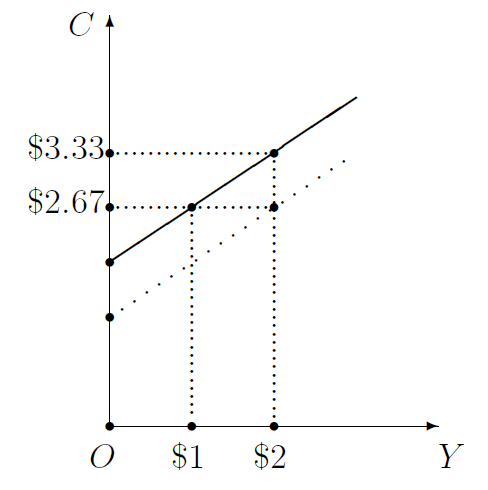
\includegraphics{images/consumption_function.png}

}

\caption{\label{fig-consumption_function}\textbf{Consumption Function}.
The solid line shows the relation between consuption spending (\(C\))
and income (\(Y\)) for some specified level of taxes (\(T\)). Note that
an increase in \(Y\) from \$1.00 to \$2.00 causes \(C\) to increase from
\$2.67 to \$3.33. (Don't be alarmed: \(C\) can exceed \(Y\) when people
dis-save (or, borrow) to spend more than what they earn.) In other
words, when \(Y\) increases by \$1.00, \(C\) increases by \$0.67,
indicating that \(\hbox{MPC}=0.67\). When \(T\) increases by \$1.00,
\(C\) decreases---at every level of \(Y\)---by the same \$0.67. That is,
an increase in \(T\) causes the entire consumption function to shift
downwards to the dotted line.}

\end{figure}%

This does not mean that consumption is assumed to change \emph{only
when} disposable income changes. Other factors may also affect
consumption. For example, if home prices---or, generally speaking, asset
prices, such as the prices of the stocks and bonds and real estate owned
by households---increase, people may feel wealthy and, as a result,
begin to save less and consume more. Changes in interest rates may also
affect the desire to save and the urge to consume.
Equation~\ref{eq-consfn} merely simplifies the story, highlights the
role of disposable income, and downplays the effect of asste prices,
interest rates, and other variables on consumption spending.

The effect of income and taxes on consumption is graphically shown in
Figure~\ref{fig-consumption_function}. Assuming taxes (\(T\)) are
unchanged, an increase in income (\(Y\)) implies an increase in
disposable income (\(Y-T\)) and, therefore, an increase in consumption
(\(C\)), as shown by the solid line in the figure. On the other hand, an
increase in \(T\) implies a decrease in \(Y-T\) at any specified level
of \(Y\). Therefore, \(C\) decreases at every \(Y\), implying a downward
shift of the consumption function, to the dotted line in
Figure~\ref{fig-consumption_function}.

\subsection{The Marginal Propensity to Consume and Ricardian
Equivalence}\label{sec-mpc}

An important point to note about the consumption function is that it is
often not enough to make the \emph{qualitative} statement that increases
in disposable income lead to increases in consumption spending: the
\emph{quantitative} magnitude of the effect can be important as well.
One could ask, ``If disposable income (\(Y-T\)) increases by one dollar
(and if all the other factors that affect consumption spending---such as
the asset prices and interest rates mentioned in the last
paragraph---remain unchanged), by \emph{how many} dollars will
consumption increase?''

The answer to this question is the \textbf{marginal propensity to
consume}. \index{marginal propensity to consume} For example, if people
spend 70 cents out of every dollar of additional disposable income and
save the remaining 30 cents, we say that the marginal propensity to
consume (MPC) is 0.70 and the \textbf{marginal propensity to save} (MPS)
is 0.30.\footnote{Note that \(0<\hbox{MPC},\hbox{MPS}<1\) and that
  \(\hbox{MPC}+\hbox{MPS}=1\), by definition.}

In Figure~\ref{fig-consumption_function}, for example, the MPC is 0.67.
As a result, when \(Y\) increases by \$1.00, \(C\) increases by \$0.67.
In general, when \(Y\) increases (respectively, decreases) by \$\(x\),
\(C\) increases (respectively, decreases) by \$0.67\(x\). On the other
hand, a one-dollar increase in \(T\) implies a one-dollar
\emph{decrease} in disposable income, causing \(C\) to \emph{decrease}
by \$0.67 at every value of \(Y\). As a result, the consumption function
shifts downward by the amount of the MPC when taxes increase by one
dollar. In general, when \(T\) increases (respectively, decreases) by
\$\(y\), the consumption function shifts down (respectively, up) by
\$0.67\(y\).

It is typically assumed that the magnitude of the MPC depends on whether
a change in disposable income is perceived to be permanent or temporary.
If the income of a household increases by \$500 a month and if this is
perceived to be a permanent increase, it is reasonable to assume that
consumption spending will also increase by nearly \$500 a month. In
other words, \emph{for changes in \(Y\) or \(T\) that are perceived to
be permanent, it is reasonable to assume \(\text{MPC}=1\) and
\(\text{MPS}=0\)}. On the other hand, if the people receive a tax cut in
the run-up to an election and come to believe that the tax cut will be
revoked once the election is over, then it is reasonable to assume that
the people will save the bonanza from the tax cut. In other words,
\emph{for changes in \(Y\) or \(T\) that are perceived to be temporary,
it is reasonable to assume \(\text{MPC}=0\) and
\(\text{MPS}=1\)}.\footnote{For a full discussion, see pages 163-5 of
  \emph{Macroeconomics: A Modern Approach} by Robert J. Barro, Thomson
  South-Western, Mason, OH, 2008.}

People's estimation of the permanence of a tax cut may also depend on
whether the tax cut is accompanied by a cut in government spending,
\(G\). If there is a cut in taxes but none in government spending, the
government would have to borrow from private lenders (for example,
banks) to make up the shortfall in tax revenue. But the borrowed money
would eventually have to be repayed---with interest. Where would the
government get the money to do so? It would probably raise
taxes.\footnote{The government could take out a new loan to repay an old
  loan. But there are limits to how far this could be continued. Lenders
  may eventually balk.} Therefore, if people are smart enough, they may
come to believe that a tax cut unaccompanied by a cut in government
spending is very likely a temporary tax cut that would lead eventually
to a tax hike larger than the tax cut itself. They may therefore respond
to the tax cut, not by going on a shopping spree, but instead by socking
the tax cut away in a bank thinking that a big tax increase is on the
way.

This sceptical view of the effect of a tax cut on consumption spending
is referred to as the theory of \textbf{Ricardian equivalence}. Let's
consider this further with a numerical example. Suppose the government
reduces taxes (\(T\)) from \$1000 to \$900 but leaves annual government
spending (\(G\)) unchanged at \$1000. The government borrows \$100 from
a bank at a 7\% interest rate to make up the shortfall in tax revenue.
Therefore, a year later the government would have to repay \$107 to the
bank. Therefore, people may conclude that the \$100 tax cut is illusory
and would inevitably be followed by a \$107 tax increase a year
later---to the level of \$1107 to pay for \$1000 in government spending
plus \$107 in loan repayment. Knowing that they would need an extra
\$107 next year, what would the people do? They would take the \$100 tax
cut and put it in a bank so that, at 7\% interest, they would have
enough next year to pay the tax hike they know is coming.

In other words, when a reduction in \(T\) is not accompanied by an equal
cut in \(G\), \(\hbox{MPC}=0\) and \(\hbox{MPS}=1\).

Another implication of the theory of Ricardian equivalence is that in
some circumstances consumption spending may respond \emph{as if} taxes
have changed even if they actually haven't! Let's say government
spending increases by \$100 but taxes stay the same. Once again, the
government would have to borrow \$100 from a bank. Therefore, a year
later it would need to raise taxes by \$107 (assuming 7\% interest, as
before) to repay the loan with interest. Therefore, taxes would have to
rise next year by \$107. Therefore, if people anticipate all this, they
would put away an extra \$100 in their bank accounts in preparation for
the \$107 tax increase they can see coming. In other words, if \(G\)
increases and \(Y-T\) remains unchanged, \(C\) would \emph{fall}, as if
the people are saying to themselves that taxes have risen even though
they actually have not.

Therefore, according to Ricardian equivalence, when analysing the effect
of a change in government spending it might be a good idea to pretend
that the change in \(G\) is accompanied by an equal change in \(T\),
even if \(T\) is actually unchanged.

\section{What Are the Factors that Affect
Investment?}\label{sec-investment}

Unlike consumption spending (\(C\)), which has been assumed above to
depend on disposable income (\(Y-T\)), the total of the investment plans
of businesses (\(I\)) is assumed, for simplicity, to dance to its own
tune, to be unrelated to other economic variables.

To use a term that will be explained in Section~\ref{sec-exovar},
investment will be assumed here to be an \emph{exogenous} variable. You
will see later that fluctuations in \(I\) can explain fluctuations in
other variables such as \(Y\). But you will see no explanation of the
fluctuations in \(I\) itself. Investment will be used here as an
explanatory variable, but it will remain unexplained itself.

In a theory that argues that increases in temperature cause increases in
murder rates, but has nothing to say about what causes temperature to
increase, temperature is exogenous and the murder rate is endogenous. In
this case, the author of the theory may be admitting that the weather is
too complex to explain. Or, perhaps she has concluded that trying to
explain the weather would be a waste of time: as we cannot control the
weather, it would make sense to forget about what causes temperature
fluctuations and instead concentrate on how to deploy the police
strategically on hot days to keep murder rates from spiking. Either way,
weather is being treated as exogenous.

Returning to the issue at hand, investment is actually not entirely
mysterious. A strong case can be made that \(I\) depends on the real
(or, inflation-adjusted) interest rate, which is the inflation-adjusted
cost of the money that businesses need to borrow in order to pay for
their investment spending.\footnote{Indeed, in a later chapter I will
  assume that real investment spending, \(I\), is inversely related to
  the real interest rate, \(r\).}

Advances in technology and increases in the quantity and quality of a
nation's work force are important influences too. When such changes
happen, the productivity of capital goods (such as equipment, machinery,
software, etc.) increases. This induces greater investment in additional
capital goods.\footnote{See chapter 17 of \emph{Macroeconomics}, sixth
  edition, by N. Gregory Mankiw, Worth Publishers, New York, NY, 2007,
  ISBN:978--0--7167--6213--3, for more on the theory of business
  investment.}

That said, most economists agree that investment spending by businesses
is overwhelmingly dependent on that elusive thing called the optimism or
the ``animal spirits'' of businesspeople. And, as business psychology is
not their strong suite, economists tend not to say much about such
things. I will simply assume that the level of investment is exogenous
or inexplicable---it is what it is.

\section{What Are the Factors that Affect Government
Spending?}\label{sec-gov}

Who knows?! Ask your Poli-Sci professor. I will treat \(G\) as a
variable that is inexplicable but nonetheless useful in explaining
changes in other variables such as \(Y\), \(C\), \(NX\), etc. In other
words, I will consider \(G\) to be exogenous---see
Section~\ref{sec-exovar}.\footnote{I should not, however, give the
  impression that factors that influence the level of government
  spending are not discussed in economic research. See
  \textcite{mueller2003public}, \textcite{persson2002political}, and
  \textcite{drazen2002political}.}

\section{What Are the Factors that Affect Net
Exports?}\label{sec-netexports}

As we saw in Section~\ref{sec-netexports-nia} and
Section~\ref{sec-goodseqmdef}, net exports is the excess of exports over
imports: \begin{equation}\phantomsection\label{eq-nxp}{
NX\equiv EX-IM,
}\end{equation} where, \(EX\) denotes the real (i.e.,
inflation-adjusted) value of the planned sales of domestically produced
goods and services\index{exports} to foreign residents, and \(IM\)
denotes the real value of the demand for foreign-made goods from
domestic residents\index{imports}. Therefore, to understand what drives
\(NX\) up and down, we need to look at what makes \(EX\) and \(IM\)
fluctuate.

\subsection{What Are the Factors that Affect
Exports?}\label{sec-exports}

I will assume that the demand from foreign residents for the goods and
services produced in the domestic economy---i.e., the domestic country's
exports---is given by

\begin{equation}\phantomsection\label{eq-exp}{
EX=EX(q),
}\end{equation} where, as was pointed out in
Section~\ref{sec-realexrates}, the real exchange rate (\(q\)) is the
amount of domestically produced goods that can be obtained in trade for
one unit of foreign-made goods. As the real exchange rate is the
relative price of foreign goods (in units of domestic goods), a rise in
\(q\) would encourage foreigners to buy more domestic goods. That is,
\emph{\(EX\) and \(q\) are directly related}.

The real exchange rate, however, is not the only thing that affects
exports. An important influence is foreign GDP. For example, countries
such as China, Japan, and Germany saw sharp declines in their exports to
the US during the US recession of 2008--09. To keep things simple,
however, I will ignore this issue and assume that \(EX\) depends on
\(q\) alone.

\subsection{What Are the Factors that Affect
Imports?}\label{sec-imports}

I will assume that the domestic country's demand for foreign-made
goods---i.e., its imports---is given by

\begin{equation}\phantomsection\label{eq-imports}{
IM=IM(q,Y-T).
}\end{equation}

Since the real exchange rate, \(q\), is the amount of domestically
produced goods that can be obtained in trade for one unit of
foreign-made goods, it should be clear that a high level of \(q\) would
discourage the import of foreign-made goods; i.e., \emph{\(q\) and
\(IM\) are inversely related}.

And, as we saw in Section~\ref{sec-consumption} above, increases in
disposable income (\(Y-T\)) lead to increases in consumption spending
(\(C\)). Part of this additional consumption is likely to consist of
foreign-made goods. Therefore, it follows in an obvious way that
\emph{\(Y-T\) and \(IM\) are directly related}. Moreover, it also
follows that when disposable income increases, consumption increases
more than imports do. That is, the marginal propensity to import is
smaller than the marginal propensity to consume.

It is also important to keep in mind that just as the effect of a change
in disposable income on consumption spending depends on whether the
change in disposable income is perceived to be permanent or
temporary---see Section~\ref{sec-mpc} for a reminder---so does the
effect of a change in disposable income on households' purchases of
imported goods.

\subsection{Summary: What Are the Factors that Affect Net
Exports?}\label{sec-summary-nxp}

Section~\ref{sec-exports} and Section~\ref{sec-imports} imply that we
can summarize the nature of a country's net exports by the equation

\begin{equation}\phantomsection\label{eq-netexports}{
NX=NX(q,Y-T).
}\end{equation}

Moreover, we can conclude that \emph{net exports (\(NX\)) is related
directly to the real exchange rate (\(q\)) and inversely to disposable
income (\(Y-T\))}.

These effects of \(q\), \(Y\), and \(T\) on \(NX\) are shown graphically
in the two panels of figure Figure~\ref{fig-net_exports_general}. The
left panel emphasizes the role of the real exchange rate in a nation's
net exports. This rising net exports curve shifts rightward when \(Y-T\)
decreases, indicating lower imports and, therefore, higher net exports
at every value of \(q\). The right panel of figure
Figure~\ref{fig-net_exports_general}, on the other hand, emphasizes the
role of GDP in determining a nation's net exports. This net exports
curve is negatively sloped, indicating that rising incomes lead to
rising imports and, therefore, falling net exports. Both graphical
representations of \(NX\) in figure Figure~\ref{fig-net_exports_general}
are useful, depending on the context.

\begin{figure}

\centering{

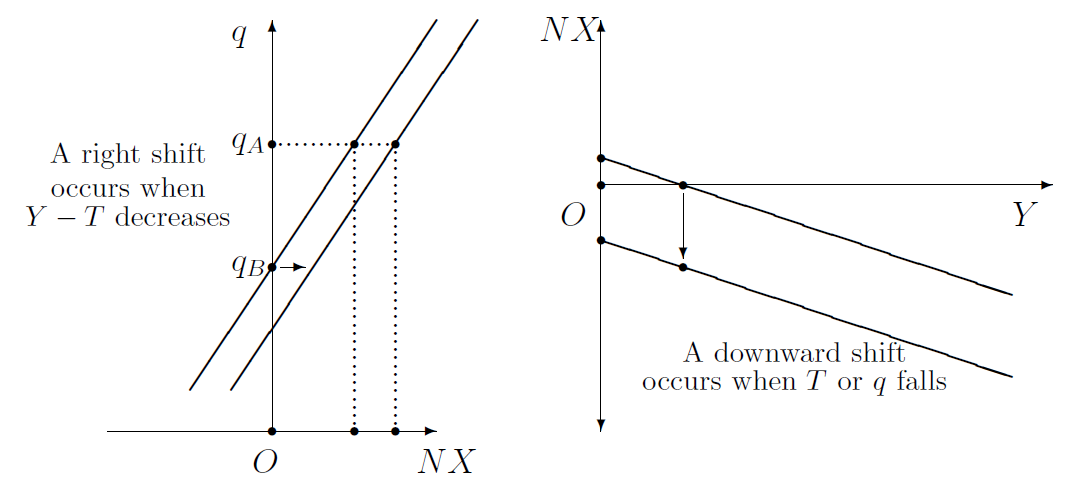
\includegraphics{images/net_exports_general.png}

}

\caption{\label{fig-net_exports_general}\textbf{Net Exports} This figure
shows that both the real exchange rate (\(q\)) and taxes (\(T\)) have a
direct effect on net exports (\(NX\)) and that GDP (\(Y\)) has an
inverse effect. The left panel highlights the effect of the real
exchange rate. This curve shifts right when \(Y-T\) decreases. The right
panel highlights the effect of real GDP. This curve shifts down when
either \(q\) or \(T\) decreases. Note that net exports could be positive
or negative. Absolute purchasing power parity is \emph{not} assumed for
this diagram.}

\end{figure}%

The direct relation between \(NX\) and \(q\) is shown one more time in
figure Figure~\ref{fig-net_exports_real_exchange_rate}. The left panel
in particular shows that as \(q\) increases from \(q_B\) to \(q_A\),
\(NX\) increases from \(NX=0\) to \(NX=NX_A\). Had the net exports curve
instead been the flatter dotted line, the same change in the real
exchange rate would have provoked a bigger change in net exports. In
other words, the flatter the net exports curve is---or, the more elastic
it is, if you can forgive the jargon---the more responsive \(NX\) is to
\(q\). In the extreme case of \emph{infinite} responsiveness or
elasticity, the net exports curve is horizontal.

If, moreover, the net exports curve is horizontal at \(q=1\), as in the
right panel of figure Figure~\ref{fig-net_exports_real_exchange_rate},
it is said to obey the \textbf{law of one price} or \textbf{absolute
purchasing power parity}. This is discussed further in the next
section.\index{purchasing power parity!absolute}

\begin{figure}

\centering{

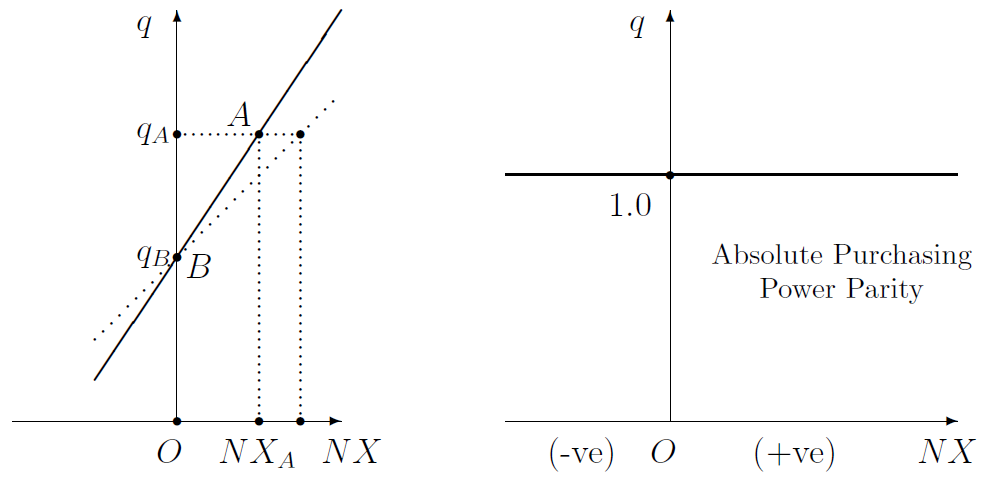
\includegraphics{images/net_exports_real_exchange_rate.png}

}

\caption{\label{fig-net_exports_real_exchange_rate}\textbf{Net Exports
and the Real Exchange Rate} The left panel shows a general direct
relation between net exports and the real exchange rate. Note that net
exports could be positive or negative. The right panel shows the
relation between net exports and the real exchange rate under the law of
one price or, equivalently, under absolute purchasing power parity.}

\end{figure}%

\subsection{The Law of One Price and Purchasing Power
Parity}\label{sec-appp}

The direct relation between net exports and the real exchange rate, when
taken to an extreme, leads to the \emph{law of one price} or,
equivalently, \emph{absolute purchasing power parity}
\index{purchasing power parity!absolute} (PPP). This requires that net
exports be infinitely elastic with respect to changes in the real
exchange rate (\(q\)) and that

\begin{equation}\phantomsection\label{eq-absppp}{
q\equiv\frac{E\cdot P^*}{P}=1.
}\end{equation}

The first equality in Equation~\ref{eq-absppp} is simply the algebraic
definition of the real exchange rate that we saw in Equation~\ref{eq-q}
of Section~\ref{sec-realexrates}. What is new in
Equation~\ref{eq-absppp} is its insistence that \(q=1\).

To see the logic behind this, let us work through an example. Suppose
the price, \(P\), of American wheat is 2 dollars per pound; the price,
\(P^*\), of French wheat is 3 euros per pound; and the price of a euro,
\(E\), is \$2.00. Therefore, the price of French wheat \emph{in US
dollars} is \(E\times P^*=2.00\times 3=6\) US dollars, thrice the price
of identical US wheat.

How likely is this situation---in which the real exchange rate is
\(q=2.00\times 3/2=3\)---to persist? Not very likely, is the clear
answer. People all over the world will see a juicy opportunity for
\textbf{arbitrage} \index{arbitrage}, which is a fancy term for the
practice of making money by buying something at a cheap price and
selling it at a higher price. People will start buying American wheat to
sell in France. As long as \(q=3\) persists, nobody will wish to sell
wheat in the US and everybody will want to make money by buying up every
grain of US wheat and selling it in France. This is clearly
unsustainable. Net exports from America to France will be literally
infinite!

On the other hand, suppose \(P=2\) dollars per pound of American wheat,
as before; \(E=2.00\) dollars per euro, also as before; but \(P^*=0.50\)
euros per pound of French wheat. Now the price of French wheat \emph{in
dollars} is \(E\times P^*=2.00\times 0.50=1\) dollar, \emph{half} the
price of identical American wheat.

How likely is this situation---in which the real exchange rate is
\(q=2.00\times 0.50/2.00=0.50\)---to persist? Again, not very likely.
People will now wish to buy every grain of French wheat for sale in
America. Net exports from America to France will now be negative
infinity, which is clearly an unsustainable situation.

For planned net exports to be neither infinity nor negative infinity,
the price of wheat must be \emph{equal} in America and France (when both
prices are measured in the same currency). This is the basic idea of
\emph{the law of one price: the price of any tradable commodity, when
measured with the same yardstick, should be the same everywhere if there
are no trade-related costs}.

To be specific, note that when I calculated the price of French wheat in
dollars in the numerical examples above, I multiplied \(E\) and \(P^*\).
Therefore, saying that the price of wheat, when measured in the same
currency, should be the same in America and France amounts to saying
that \[
E\cdot P^* = P,
\] which in turn implies \(q=1\) or absolute purchasing power parity, as
in Equation~\ref{eq-absppp}.

Note also that as the magnitude of America's net exports is infinity
when American goods are cheaper than French goods (\(q>1\)) and negative
infinity when American goods are pricier than French goods (\(q<1\)), a
finite level of net exports is possible only when \(q=1\). This is
graphically represented by the \emph{horizontal} net exports curve in
the right panel of Figure~\ref{fig-net_exports_general}.

The notion of absolute purchasing power parity does have a common-sense
appeal. Unfortunately, it doesn't seem to fit the facts very well,
partly because many goods and services (haircuts and dry cleaning, for
example) are not traded across large distances. Real exchange rates have
been observed to stay higher than 1.0 (or lower than 1.0) for long
periods of time. Therefore, in these lectures, I will \emph{not} assume
absolute purchasing power parity. Instead, a less stringent version of
the idea---\emph{relative} purchasing power parity---will be
used.\footnote{See Section~\ref{sec-rppp} of Chapter~\ref{sec-longnom}.
  \index{purchasing power parity!relative}}

\section{Summary: What Is the Goods Market Equilibrium
Condition?}\label{sec-summary-goodseqm}

Using Equation~\ref{eq-goodseqm} -- Equation~\ref{eq-imports}, the goods
market equilibrium condition \(Y=C+I+G+NX\) becomes:
\begin{equation}\phantomsection\label{eq-IS}{
\fbox{$\displaystyle Y=C(Y-T)+I+G+NX(q,Y-T).$}
}\end{equation}

As was pointed out in Section~\ref{sec-useeqmcon}, the goods market is
said to be in equilibrium when the supply plans of domestic producers
are equal to the demand plans of the buyers of domestically produced
goods. For this to be true, Equation~\ref{eq-IS} must be satisfied.

\section{What is the Money Market Equilibrium
Condition?}\label{sec-moneyeqm}

The \textbf{money market equilibrium condition} \index{markets!assets}
requires that the financial assets that are held by the people be held
willingly, and not under some sort of compulsion. For that to be the
case, \emph{money supply must be equal to money demand}
\index{equilibrium!money market}.

\subsection{What Is the Money Supply?}\label{sec-msupply}

Roughly, the nation's money supply\index{money!supply of} at any given
moment is the total amount of \textbf{liquid assets}
\index{asset!liquid}---that is, assets that can easily be used to pay
for purchases when you go shopping---that are held by private citizens
at that moment. A popular measure of money supply is M1. It consists of
all currency in private hands and all the money in people's checking
accounts. You may think of M1 as the maximum amount of money that people
would be able to spend if they all went shopping this minute. See
Figure~\ref{fig-M1-post2000-fredgraph} for recent trends in M1 for the
United States. For instance, on October 22, 2012, M1 was an estimated
\$2,417.2 billion, of which \emph{currency in private hands} was
\$1,079.2 billion, \emph{total checkable deposits} was \$1,334.0
billion, and \emph{travelers checks outstanding} was \$3.9 billion.

\begin{figure}

\centering{

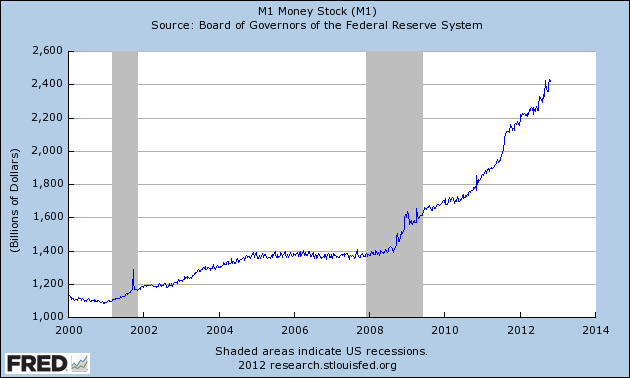
\includegraphics{images/M1-post2000-fredgraph.png}

}

\caption{\label{fig-M1-post2000-fredgraph}One measure of money supply is
M1. Here we see recent US data on M1. Note that the Federal Reserve's
actions tend to sharply boost money supply in recessions. We will see
why in later chapters. Source:
\url{https://fred.stlouisfed.org/series/M1SL}.}

\end{figure}%

As we saw in Section~\ref{sec-monetary}, I will denote money supply by
the symbol \(M\).

\subsection{What Are the Factors that Affect Money
Supply?}\label{sec-msupplydet}

A nation's money supply is controlled by its central bank.\footnote{See
  Section~\ref{sec-finacc}.}
\index{central banks!control of money supply} Recall that M1, the
simplest measure of \(M\), is basically equal to the currency held by
the public and the value of all checkable bank accounts. The central
bank can use its power to affect both these components of M1. The
central bank is the only institution that can print (or mint) currency.
Therefore, the ``currency held by the public'' can increase only if the
central bank buys something from John or Jane Q. Public and pays for it
with newly printed cash.

For instance, if Jane decides to sell some of the government bonds that
she owns, she may end up selling her bonds to the central bank in return
for a bunch of newly printed currency notes. This would imply an
increase in the currency held by the public and, therefore, in M1. Or,
it could be that John has some yen that he wishes to sell in return for
dollars. John could end up selling his yen to the U.S. central bank,
which is known as the Federal Reserve or, simply, The Fed. Again, he
would be paid in crisp newly printed dollar bills, the currency held by
the public would increase, as would M1.

Of course, the central bank could just as easily decide to sell some of
its financial assets. In that case, the above process would work in
reverse and M1 would decrease. If the Fed decides to sell some of the
government bonds it owns, the buyer could be one John Q. Public. In this
case, John would hand over some not-so-crisp dollar bills from his
wallet to the Fed as payment for the bonds he had just purchased.
Consequently, the currency held by the public would decrease, as would
M1.

Apart from controlling the currency held by the public in the manner
just outlined, a central bank indirectly controls ``the value of all
checkable bank accounts'', which is the other component of M1. This is
because a central bank typically has the power to regulate the lending
behavior of banks. If I walk into a bank and deposit a hundred dollars
into my account, the bank manager would lend \(X\) dollars out of the
money I had deposited to someone who wants a loan. That man may use the
\(X\) dollars he had borrowed to buy a shirt, in which case those \(X\)
dollars would end up in the shirt seller's checkable bank account.
Therefore, M1 would increase by \(X\) dollars. In other words, the
lending of depositors' money by banks can affect M1.

And that's where the central bank can use its regulatory power to
control the value of all checkable bank accounts and, thereby, M1. The
central bank can set limits on how much of my hundred-dollar deposit my
bank could lend. By adjusting the limit the central bank can encourage
the manager of my bank to lend more or less than \(X\) dollars to the
guy who wanted a loan. Thereby, the central bank can (indirectly)
control the rate at which bank lending expands M1.

In some cases, central banks give up control over the money supply in
order to exert control over some other economic variable that they
consider important to control. You will see in Chapter~\ref{sec-exchsys}
that in what are called fixed exchange rate systems, the central bank
can fix the value of a currency by credibly promising to buy and/or sell
that currency at the target rate of exchange. For example, if the
central bank of Thailand wishes to fix the exchange value of the Thai
baht at 25 bahts per US dollar, it can do so by announcing that it is
ready to buy and/or sell US dollars at the rate of 25 bahts per dollar.
After that announcement, the market price of a dollar could not be, say,
27 baht because nobody would buy a dollar at that price when Thailand's
central bank is willing to sell dollars for less. Similarly, the price
of a dollar could not be 23 baht because nobody would sell at that price
given that they could instead sell dollars to the Thai central bank for
a higher price. In short, once Thailand's central bank makes a credible
announcement that it will exchange one dollar for 25 baht, the market
exchange rate of a dollar will quickly become 25 baht.

However, the Thai central bank's efforts to control the exchange rate of
the baht must come at the expense of its total loss of control over
Thailand's M1. If people show up with dollars and ask for baht, the
central bank would have to print some additional currency. So, currency
held by the public would increase, as would M1. If some Thai citizens
hand over their baht and ask for dollars, the central bank would have to
dig into its dollar reserves to keep its promise. The baht held by the
thai public would decrease (because they have exhanged some of their
baht for dollars), as would M1. In this way, the central bank would gain
some control over the exchange rate, but by giving up control over M1.
M1 would now fluctuate not according to the wishes of the Thai central
bank but in tune with economic conditions in Thailand or, indeed, the
world at large.

\subsection{What Is the Money Demand?}\label{sec-mdemand}

The nation's money demand \index{money!demand for} at a specified point
in time is the total amount of liquid assets---that is, currency plus
checkable bank accounts---that its residents would like to hold at that
point in time.

\subsection{What Are the Factors that Affect the Demand for
Money?}\label{sec-mdemanddet}

The behavior of the demand for money is assumed to be described by the
equation \[
\text{Money Demand}=L(R)\cdot P\cdot Y.
\]

In other words, the demand for money is assumed to be a multiple \(L\)
of nominal income (\(P\cdot Y\); see Equation~\ref{eq-nomGDP} of
Section~\ref{sec-IPDGDP}). Moreover, the multiple \(L\) itself depends
on the nominal interest rate (\(R\)).

\subsubsection{What Are Nominal Interest Rates?}\label{sec-nomint}

The nominal interest rate, denoted by \(R\) for the domestic country and
\(R^*\) for the foreign country, is the fraction of each currency unit
borrowed (dollar, yen, etc.) that will have to be paid as
interest.\footnote{Recall from Section~\ref{sec-notnfornvar} that the
  variables that describe a foreign country have an asterisk (*)
  attached as a superscript.} If the bank charges you 15\% interest on a
loan, then the nominal interest rate is \(R=0.15\) because that is the
fraction of each dollar borrowed that you will have to pay as interest.

\subsubsection{Again, What Are the Factors that Affect the Demand for
Money?}\label{sec-mdemanddet2}

As is clear from the equation above, \emph{the demand for money is
assumed to vary directly with \(P\) and \(Y\)}. This makes sense. If,
other things being unchanged, the average price level (\(P\)) goes up,
wouldn't you wish to keep a larger part of your wealth as cash in your
wallet? Of course, you would. And if GDP (\(Y\)) increases, wouldn't
people carry more cash in their wallets? Of course, they would. A higher
real GDP implies that more goods and services are being produced and
then bought and sold. All this extra buying and selling will require
people to carry more cash with them on a regular basis.

And, as for the effect of \(R\) on money demand, if the nominal interest
rate increases, wouldn't you wish to keep less of your wealth in cash?
Yes, you would. Keep in mind that liquid assets, such as cash and
checking account deposits, are convenient when you need to go shopping,
but earn little or no interest. \emph{The nominal interest rate \(R\) is
the interest rate on non-liquid assets} \index{interest rate!nominal},
such as bonds. So, a higher nominal interest rate increases the
attractiveness of non-liquid assets and thereby reduces the desirability
of liquid assets. Therefore, \emph{\(R\) and \(L\)---and, therefore,
\(R\) and money demand---are inversely related}.\footnote{The factor
  \(L\) is the reciprocal of what is called the \textbf{velocity of
  money} or the income velocity of money, \(V\). That is, \(L=1/V\). The
  velocity is defined as the average number of times per period that a
  unit of currency is used in the purchase of a final good or service.
  For example, if the average dollar bill changes hands 10 times per
  month, then \(V=10\).}

Other factors matter too. For example, in an economic crisis, when
people are unsure that borrowers will be able to repay their loans, they
may keep more of their wealth in the form of cold hard cash instead of
lending it to others. On the other hand, when people are wealthier, they
would very likely carry more cash.\footnote{During the recession of
  2008--09, many people who had borrowed money to buy homes, defaulted
  on their loans when home prices, which they had thought would keep
  rising, fell instead. This shocking rise in loan defaults made lenders
  afraid to lend money. The sudden decline in the availability of loans
  made it hard for businesses to borrow money to expand. The sales of
  new homes and cars fell sharply because consumer loans dried up. All
  this led to sharp declines in real GDP and sharp rises in unemployment
  in the US. These troubles in the US had serious negative effects on
  other countries as well.}

\subsection{Summary: What Is the Money Market Equilibrium
Condition?}\label{sec-summary-moneyeqm}

The necessary equality of the supply and demand for money gives us what
is usually called the \textbf{money market equilibrium condition}
\index{equilibrium!money market}:

\begin{equation}\phantomsection\label{eq-LM}{
\fbox{$\displaystyle M=L(R)\cdot P\cdot Y.$}
}\end{equation}

\section{What Is the Equilibrium Condition for the Foreign Exchange
Market?}\label{sec-forexeqm}

Foreign exchange markets are said to be in equilibrium
\index{equilibrium!foreign exchange market} if, for any two currencies
\(A\) and \(B\), the amount of Currency \(A\) supplied---by those who
wish to sell Currency \(A\) in exchange for Currency \(B\)---is equal to
the amount of Currency \(A\) demanded---by those who wish to sell
Currency \(B\) in exchange for Currency \(A\). For this to be true,
\textbf{uncovered interest arbitrage} must not be possible.

People may wish to exchange currency \(A\) for currency \(B\) for many
reasons. They may be tourists who have currency \(A\) but wish to travel
in regions where currency \(B\) is accepted. They may be people who have
currency \(A\) but wish to buy goods, services, or assets from people
who accept only currency \(B\). However, I will focus on one particular
reason why people trade currencies: it involves speculation (or, less
politely, financial gambling) and is called uncovered interest
arbitrage. The foreign currency markets are in equilibrium when the
demand and supply from these speculators are perfectly matched.

\subsection{What Is Uncovered Interest Arbitrage?}\label{sec-UIA}

Opportunities for uncovered interest
arbitrage\index{uncovered interest arbitrage} are said to exist if one
can expect to profit by borrowing money in country \(A\) and lending it
to borrowers in country \(B\), or vice versa.\footnote{In the business
  press, uncovered interest arbitrage is also referred to as the ``carry
  trade.'' See, for example, ``Why the `Carry Trade' Is Back,'' by Neil
  Shah, The Wall Street Journal, August 18, 2009,
  \url{https://www.wsj.com/articles/SB125053694840237795}.
  \index{uncovered interest arbitrage!carry trade}} If this is possible,
then there would be no equilibrium in the foreign exchange market.
Profit seekers would be constantly borrowing money in country \(A\) and
then changing it into the currency of country \(B\) for the purpose of
lending it to borrowers in that country. There would be literally
\emph{no limit} to the amount of country \(A\)'s currency supplied by
these people and---for the same reason---no limit to the amount of
country \(B\)'s currency demanded by these people. As a result, the
supply of country \(A\)'s currency would necessarily exceed the demand
for it. Such a situation would not represent equilibrium.

Therefore, for equilibrium in foreign exchange markets, there must not
exist any opportunities for uncovered interest arbitrage. Put another
way, the \textbf{uncovered interest parity}
\index{uncovered interest parity} condition must be satisfied.

\subsection{What Is the Uncovered Interest Parity
Condition?}\label{sec-UIP}

The uncovered interest parity condition (UIP, for short) is that
\begin{equation}\phantomsection\label{eq-UIP}{
R=R^*+\frac{E^e_f-E}{E}
}\end{equation} must be satisfied.

As we saw in Section~\ref{sec-nomint} above, \(R\) is the nominal
interest rate in the home country, whereas \(R^*\) is the nominal
interest rate in the foreign country. As we saw in
Section~\ref{sec-nomexrates}, \(E\) is the current value of the foreign
currency in units of the domestic currency. And, as we saw in
Section~\ref{sec-forward-exp}, \(E_f\) is the future value of the
foreign currency, and \(E_f^e\) is the current expectation of the future
value of the foreign currency.\footnote{Note that, I have quietly
  assumed that everybody has the same expectation for the future value
  of the foreign currency; no differences of opinion are allowed. Also,
  you may recall that \(E_f^e\) was introduced earlier in
  Section~\ref{sec-forwardexrates}.}

Note that \(E^e_f-E\) is the expected increase in the exchange value of
the foreign currency. It then follows---along the lines of
Equation~\ref{eq-f-growthrate} in Section~\ref{sec-notngrowth} --- that
\begin{equation}\phantomsection\label{eq-eeg}{
\begin{eqnarray}
E^e_g&\equiv&\frac{E^e_f-E}{E}\nonumber \\
&\equiv&\frac{E^e_f}{E}-1
\end{eqnarray}
}\end{equation} is the expected proportional \emph{rate of increase} of
the exchange value of the foreign currency. The uncovered interest
parity equation above can therefore be written compactly as
\begin{equation}\phantomsection\label{eq-UIP-compact}{
R=R^*+E_g^e.
}\end{equation}

The second term on the right-hand side, \(E_g^e\), is often called the
\textbf{expected rate of appreciation} of the foreign currency
\index{exchange rate!appreciation}. When the exchange value of a
currency increases (respectively, decreases), the currency is said to
have appreciated (respectively, depreciated)
\index{exchange rate!depreciation}.\footnote{Similarly,
  \(100\times[(E^e_f-E)/E]\) is the expected percentage rate of increase
  of the exchange value of the foreign currency. Note that when
  \(E^e_f<E\), we have a \emph{negative} expected increase, which is the
  same as a decrease.}

With the definitions of the variables in Equation~\ref{eq-UIP} out of
the way, we can now try to understand why that equation makes sense.

\subsubsection{Why Is Uncovered Interest Parity Necessary for
Equilibrium?}\label{sec-summary-UIP}

To see the meaning of Equation~\ref{eq-UIP} above, consider the prospect
of borrowing US dollars from someone in America today, turning it into
euros in the foreign exchange market, lending it to someone in Europe
for a year, turning the euros received a year later (as principal and
interest on the loan that was made) back into dollars, paying off the
dollars that had been borrowed a year earlier, and keeping any profits
or losses that remain.

The downside of this plan is that you would have to pay interest \(R\)
on the money you borrowed in America. This is on the left-hand side of
the UIP equation; i.e., Equation~\ref{eq-UIP}.

But there is an upside too. You will get interest \(R^*\) from your
borrowers in Europe.

And that is not all. Remember that the plan requires you to change your
borrowed dollars into euros today and then change your euros back into
dollars a year later. So, you would make some money if the nominal value
of the euro, \(E\), grows during the year. For example, if \(E = 2\)
today, you would pay \$2.00 for every euro you buy today. And if
\(E_f^e = 4\) a year later, you would be able to turn each euro you have
into \$4.00. So, if \(E\) grows from \(E = 2\) at the beginning of the
year to \(E^e_f = 4\) at the year's end, you could turn \$2.00 into
\$4.00 over that year. In general, \(E^e_g\equiv(E^e_f-E)/E\) represents
your expected gains from changing dollars into euros and back into
dollars a year later.

Therefore, the right-hand side of the UIP equation above---i.e.,
\(R^* + E^e_g\)---represents your total gains from this convoluted
scheme of borrowing dollars, changing it into euros, earning interest on
those euros for a year, and finally changing the euros back into dollars
and bringing the money home.

Had the left-hand side (\(R\)) been smaller than the right-hand side
(\(R^* + E^e_g\)), opportunities for uncovered interest arbitrage would
have existed. That is, you (and everybody else in the world) would have
profited from borrowing in America and lending that money in Europe. But
that would have violated the equilibrium condition for the foreign
exchange markets.

In the same way, it can be shown that had the left-hand side been
greater than the right-hand side, opportunities for uncovered interest
arbitrage would once again have existed. Only, this time you would
expect to gain by borrowing in Europe and lending in America.

So, for equilibrium in the foreign exchange market, the two sides of
Equation~\ref{eq-UIP} would have to be equal. That is, for equilibrium
in the foreign exchange market, the uncovered interest parity condition
must be satisfied. This can be expressed either by Equation~\ref{eq-UIP}
or, equivalently, by \begin{equation}\phantomsection\label{eq-UIP-alt}{
\fbox{$\displaystyle R=R^*+\frac{E^e_f}{E}-1.$}
}\end{equation}

\subsubsection{Perfect Capital Mobility}\label{sec-pcm}

My discussion of the uncovered interest parity condition in
Section~\ref{sec-summary-UIP} has implicitly assumed perfect capital
mobility\index{perfect capital mobility} in foreign exchange markets.
This requires that:

\begin{itemize}
\tightlist
\item
  All individuals have the same expectations, and
\item
  When considering which assets to buy and which assets to sell, people
  only look at the long-run average returns of the various available
  assets.\footnote{The long-run average return of an asset is also
    called the mathematical expectation\index{expectation, mathematical}
    of the returns of the asset.}
\end{itemize}

The first requirement was discussed in Section~\ref{sec-UIP} on
\(E_f^e\).

The second requirement of perfect capital mobility is that the long-run
average return of an asset is all that we care about when judging the
attractiveness of an asset. This idea is implicit in the discussion of
uncovered interest parity in Section~\ref{sec-summary-UIP}. If you
borrow money in America and lend it in Europe, the benefits of all this
wheeling and dealing are measured by \(R^*+[(E^e_f-E)/E]\). This is just
the long-run average return that you would expect to receive. The UIP
equation, Equation~\ref{eq-UIP}, therefore, reflects what equilibrium in
foreign exchange markets ought to look like if these long-run average
returns are all that matter to people.

Perfect capital mobility, therefore, implies that the UIP equation must
be satisfied for the foreign exchange market to be in equilibrium.

We need to remember, however, that although I have assumed perfect
capital mobility, I did so just for simplicity. In the real world,
perfect capital mobility is unlikely to be true. First of all, different
people cannot be expected to have the same expectations. Secondly, in
judging the attractiveness of an asset, people are likely to look not
only at the asset's long-run average return but also at the volatility
(or variability, or dispersion, or riskiness) of the asset's return.
Consider asset \(A\), which gives a steady 5\% return, and another
asset, asset \(B\), which yields a 0\% return half the time and a 10\%
return half the time, for a long-run average return of 5\%. Assets \(A\)
and \(B\) both have the same long-run average return of 5\%. And yet,
most people will not regard assets \(A\) and \(B\) to be equally
attractive; most people will regard asset \(A\) to be superior because
it is less risky.

In my justification of uncovered interest parity in
Section~\ref{sec-summary-UIP}, I focused on the long-run average returns
and ignored the riskiness of assets. For example, I assumed that people
consider \((E^e_f-E)/E\), the expected appreciation of the foreign
currency, but ignore the fact that even if people have an expectation
about how much that currency may appreciate, they will also be aware
that that expectation is just that, an expectation.

Therefore, one needs to keep in mind the limitations inherent in
defining equilibrium in foreign exchange markets by
Equation~\ref{eq-UIP}.

\section{Summary: The Basic Equations}\label{sec-summary-basiceq}

To sum up, the theory of international macroeconomics that I am
discussing here---which, incidentally, is called the Mundell-Fleming
theory after the names of its authors---relies on three basic equations:

\begin{itemize}
\tightlist
\item
  \textbf{The goods market equilibrium equation} that must be satisfied
  if the demand for domestically produced goods is to be equal to the
  supply of such goods. See Equation~\ref{eq-goodseqm}, and
  Equation~\ref{eq-IS} for equivalent versions of this equation.
\item
  \textbf{The money market equilibrium equation} that must be satisfied
  if the demand for money is to be equal to the supply of money. See
  Equation~\ref{eq-LM}.
\item
  \textbf{The foreign exchange market equilibrium equation} that must be
  satisfied if the demand for foreign currencies is to be equal to the
  supply of foreign currencies. See Equation~\ref{eq-UIP} and
  Equation~\ref{eq-UIP-alt} for equivalent versions of this equation.
\end{itemize}

\bookmarksetup{startatroot}

\chapter{Theories, Equations and Variables}\label{sec-theqvar}

\section{What Is a Theory?}\label{sec-theory}

For my purposes, a theory\index{theory} is anything that consists of

\begin{itemize}
\tightlist
\item
  a list of exogenous variables,
\item
  a list of endogenous variables, and
\item
  a bunch of equations that show how the variables are related to each
  other.
\end{itemize}

If a theory is to be useful, its equations will help us predict how the
\textbf{endogenous variables} \index{variables!endogenous} are affected
by changes in the \textbf{exogenous variables}
\index{variables!exogenous}.

\subsection{What Are Exogenous Variables?}\label{sec-exovar}

\emph{A variable is said to be exogenous to a theory if the theory does
not seek to explain the ups and downs of the variable.}

Consider a theory of, say, the crime rate that says that a city's crime
rate goes up (respectively, down) when it has less (respectively, more)
rain, but is totally silent about why the amount of rain itself might go
up or down. For such a theory, the amount of rain is an exogenous
variable.\footnote{Lest you think that such a theory is too far fetched,
  see ``In New York City, Fewer Murders on Rainy Days,'' by ANDREW W.
  LEHREN and CHRISTINE HAUSER, The New York Times, July 2, 2009,
  \url{https://www.nytimes.com/2009/07/03/nyregion/03murder.html}.}

Exogenous variables are basically of two types: \textbf{policy
variables} \index{variables!exogenous!policy variables} and
\textbf{shocks} \index{variables!exogenous!shocks}. Policy variables are
those exogenous variables whose values can be raised or lowered by
policy makers or administrators in the government. All other exogenous
variables are called shocks.

\subsection{What Are Endogenous Variables?}\label{sec-endovar}

\emph{A variable is endogenous to a theory if the theory aims to explain
why that variable might increase or decrease}.

In the example that was just considered, the crime rate is the
endogenous variable.

\subsection{How Many Equations Are Enough?}\label{sec-howmanyeq}

Recall that a theory must have a set of equations that show how the
various exogenous and endogenous variables are related to each other.
The question now is: How many equations should a theory have? And the
short answer is: as many equations as are necessary to enable the theory
to do what it is supposed to do, which is to predict the up/down
movements of the theory's endogenous variables.

To predict whether a particular endogenous variable would increase or
decrease if some exogenous variable, say, increases from a low value to
a high value, we would need to be able to pin down the values taken by
the endogenous variable at the low and high values of the exogenous
variable. Once that is done it would become clear whether the increase
in the exogenous variable causes the endogenous variable to increase or
decrease or stay unchanged. To illustrate with the theory of crime that
we discussed earlier, if the equations in that theory of crime allow us
to pin down the value of the crime rate both when the amount of rain is
high and when the amount of rain is low, then we would know how an
increase (or decrease) in the amount of rain would affect crime.

\begin{theorem}[Solving
Equations]\protect\hypertarget{thm-eqnno}{}\label{thm-eqnno}

To pin down the values of the various endogenous variables of a theory
we in general need exactly as many equations as there are endogenous
variables: not more, not less. If there are more endogenous variables
than there are equations, we would generally get many possible
solutions, and that would make it impossible to say anything definite.
If there are fewer endogenous variables than there are equations we
would generally get no solutions at all.

\end{theorem}

To see this idea in action, let us try some numbers. Let's say a theory
has

\begin{itemize}
\tightlist
\item
  two endogenous variables, \(x\) and \(y\), and
\item
  three exogenous variables \(a\), \(b\) and \(c\).
\end{itemize}

\textbf{Case 1} Let's suppose that the theory consists of just
\emph{one} equation: \begin{equation}\phantomsection\label{eq-first}{
x + y = a + \frac{b}{c}.
}\end{equation} Assume that \(a = 3\) and \(b = c = 6\). It should then
be clear that it is impossible to pin down a unique set of values for
\(x\) and \(y\). For example, (\(x = 2\) and \(y = 2\)), (\(x = 3\) and
\(y = 1\)), and (\(x = 1\) and \(y = 3\)) are only three of infinitely
many sets of values for \(x\) and \(y\) that are solutions to
Equation~\ref{eq-first} in this case.

Now, the whole point of a theory is to predict how changes in the
exogenous variables affect the endogenous variables. For example, one
might ask what would happen to \(x\) if \(b\) increased from 6 to 12.
Answering this question would be easy if there existed a unique value of
\(x\) when \(a=3\), \(b=6\) and \(c=6\) and a unique value of \(x\) when
\(a=3\), \(b=12\) and \(c=6\). Unfortunately, Equation~\ref{eq-first}
can't tell us what \(x\) is when \(a = 3\), \(b = 6\) and \(c = 6\) and
or what \(x\) is when \(a = 3\), \(b = 12\) and \(c = 6\). We,
therefore, see that if a theory's equations can't give us unique
solutions for the theory's endogenous variables, then that theory is
useless.

\textbf{Case 2} Let's now suppose that the theory consists of
\emph{three} equations---Equation~\ref{eq-first} above and the two
equations below: \begin{equation}\phantomsection\label{eq-second}{
x - y = a - \frac{b}{c}
}\end{equation}

\begin{equation}\phantomsection\label{eq-third}{
x  = a -c
}\end{equation}

It should be clear that it is impossible, in general, to find \emph{any}
values of the endogenous variables \(x\) and \(y\) that would satisfy
all three equations. For \(a=3\) and \(b=c=6\), the equations become \[
\begin{eqnarray*}
x + y &=& 4\\
x - y &=& 2\\
x &=& -3
\end{eqnarray*}
\] respectively. If you try a few numbers, you will soon see that not
all three equations can simultaneously be satisfied. If you substitute
\(x = -3\), which is the third equation, into the first equation, you'll
get \(y = 7\). But in that case the second equation cannot be satisfied
because \(x - y\) would be -10, not 2, which is what the second equation
requires.

\textbf{Case 3} If, however, the theory has two equations---the same
number as the number of endogenous variables---a unique set of solutions
for the endogenous variables can usually be found. Let's say the
theory's equations are Equation~\ref{eq-first} and
Equation~\ref{eq-second} above, but not Equation~\ref{eq-third}. Then it
is clear that \(x = 3\) and \(y =1\) solve Equation~\ref{eq-first} and
Equation~\ref{eq-second} when \(a=3\), and \(b=c=6\).\footnote{Those of
  you who have taken linear algebra may recall the distinction between
  dependent and independent sets of linear equations. For a set of
  linear equations to have unique solutions for its endogenous
  variables, the number of independent equations must equal the number
  of endogenous variables. Although I have not been explicit,
  Theorem~\ref{thm-eqnno} really holds when the equations that we are
  talking about are linear and independent of each other.}

\section{What Can We Do With a Theory?}\label{sec-whytheory}

Let us consider further the theory that consists of
Equation~\ref{eq-first} and Equation~\ref{eq-second}. I have shown that
this theory can tell us the numerical values of its endogenous
variables, \(x\) and \(y\), whenever the numerical values of its
exogenous variables, \(a\), \(b\), and \(c\), are known. The question
now is: What can we \emph{do} with this theory?

The short answer is that we can predict the \textbf{ceteris paribus
effects} of the exogenous variables on the endogenous variables. A
change in an exogenous variable is called a \textbf{ceteris paribus
change} if all other exogenous variables are unchanged. A theory enables
us to predict how a ceteris paribus change in an exogenous variable
affects all the endogenous variables.

It is straightforward to check that if \(b\) increases from 6 to 12 and
\(a\) and \(c\) remain unchanged at 3 and 6 respectively, \(x\) would
remain unchanged at 3 and \(y\) would increase from 1 to 2. (As an
exercise, work out the values of \(x\) and \(y\) from
Equation~\ref{eq-first} and Equation~\ref{eq-second} for \(a = 3\),
\(b = 12\) and \(c = 6\).) Thus, our theory is able to predict how the
endogenous variables, \(x\) and \(y\), would behave if the exogenous
variables---\(a\), \(b\) and \(c\)---change in some specified manner.

To see this in another way, note that Equation~\ref{eq-first} and
Equation~\ref{eq-second} can be solved in terms of \(a\), \(b\) and
\(c\). In other words, one can write down the values of \(x\) and \(y\)
that solve Equation~\ref{eq-first} and Equation~\ref{eq-second} as
expressions involving \(a\), \(b\) and \(c\). Specifically, it is
straightforward to check that Equation~\ref{eq-first} and
Equation~\ref{eq-second} imply:
\begin{equation}\phantomsection\label{eq-y}{
\begin{eqnarray}
x &=& a \\
y &=& \frac{b}{c}
\end{eqnarray}
}\end{equation}

As an exercise, substitute \(x=a\) and \(y=b/c\) in
Equation~\ref{eq-first} and Equation~\ref{eq-second} and show that the
two sides of each equation become the same. This would verify my claim
that these values of \(x\) and \(y\) do indeed solve
Equation~\ref{eq-first} and Equation~\ref{eq-second}.

We can now complete our discussion of the utility of theories by noting
that the solutions \(x=a\) and \(y=b/c\) imply that:

\begin{itemize}
\tightlist
\item
  \(x\) is directly related to \(a\) and unrelated to \(b\) and \(c\),
  and\footnote{There is a \textbf{direct relation} between an exogenous
    variable \(a\) and an endogenous variable \(x\) if a ceteris paribus
    increase (respectively, decrease) in \(a\) causes an increase
    (respectively, a decrease) in \(x\). Conversely, there is an
    \textbf{inverse relation} between an exogenous variable \(a\) and an
    endogenous variable \(x\) if a ceteris paribus increase
    (respectively, decrease) in \(a\) causes a decrease (respectively,
    an increase) in \(x\).}
\item
  \(y\) is directly related to \(b\), inversely related to \(c\)---that
  is, a ceteris paribus increase (respectively, decrease) in \(c\)
  causes a decrease (respectively, an increase) in \(y\)---and unrelated
  to \(a\).
\end{itemize}

Table~\ref{tbl-xyabc} reports these ceteris paribus effects in another
format. This tabular format will be used frequently in future lectures.

\begin{longtable}[]{@{}ccc@{}}
\caption{\textbf{Predictions of the theory consisting of}
Equation~\ref{eq-first} and Equation~\ref{eq-second}. All variables
named in the first column are exogenous and all variables listed in the
first row are endogenous. Each cell in the table shows the relation
between the exogenous variable and the endogenous variable aligned with
the cell. The +/- symbols denote a direct/inverse relation and a zero
denotes that there is no relation.}\label{tbl-xyabc}\tabularnewline
\toprule\noalign{}
& \(x\) & \(y\) \\
\midrule\noalign{}
\endfirsthead
\toprule\noalign{}
& \(x\) & \(y\) \\
\midrule\noalign{}
\endhead
\bottomrule\noalign{}
\endlastfoot
\(a\) & + & 0 \\
\(b\) & 0 & + \\
\(c\) & 0 & - \\
\end{longtable}

We see that the theory we've been considering provides a full set of
testable predictions about how its endogenous variables would behave for
any given change in its exogenous variables. Once we have a theory that
provides testable predictions, that's when the hard work of actually
testing those predictions begins. You'll have to find historical data on
\(x\), \(y\), \(a\), \(b\) and \(c\)---this may require long hours in
the library!---and check whether the data support the predictions in
Table~\ref{tbl-xyabc}. If they don't, you need to get cracking on a new
theory with new variables and/or equations. On the other hand, if the
data support the predictions in Table~\ref{tbl-xyabc}, you may have a
publishable paper. At that point, you would need to be careful not to
let the associated fame and fortune go to your head.

\bookmarksetup{startatroot}

\chapter{The Long Run and the Short Run}\label{sec-shortlong}

\section{In Our Three Basic Equations, Which Variables Are Exogenous and
Which Are Endogenous?}\label{sec-exoendo}

My discussion of international macroeconomic theory has, so far,
described three equations that represent equilibrium in the goods,
money, and foreign exchange markets.\footnote{See
  Section~\ref{sec-summary-basiceq}.} So, for the theory to work, there
would have to be exactly three endogenous variables.\footnote{See
  Theorem~\ref{thm-eqnno} in Section~\ref{sec-howmanyeq}.} So, we need
to start figuring out which variables in those three equations are
exogenous and which are endogenous and check how many endogenous ones
there are.

The list of variables that you have seen so far is already pretty long:
\(G\), \(T\), \(M\), \(q\), \(Y\), \(C\), \(I\), \(NX\), \(EX\), \(IM\),
\(E\), \(E^e_f\), \(R\), \(R^*\), \(P\), and \(P^*\). The question is:
Which of these are endogenous and which are exogenous?\footnote{Recall
  from Section~\ref{sec-exovar} and Section~\ref{sec-endovar} that
  endogenous variables are the variables whose ups and downs are
  explained by the theory and exogenous variables are the variables that
  the theory does not consider to be any of its business.}

The \emph{variables that will always be exogenous in these lectures} are
\(I\), \(G\), and \(T\). Moreover, all variables that describe the
foreign country (\(R^*\) and \(P^*\)) will also be regarded as
exogenous.

The \emph{variables that will always be endogenous in these lectures}
are \(Y\), \(C\), \(I\), \(NX\), \(EX\), \(IM\), \(q\), and \(R\).

As for the other variables, whether they are exogenous or endogenous
will depend on two issues:

\begin{itemize}
\tightlist
\item
  Do we want to do long-run analysis or short-run analysis? and
\item
  Does the domestic economy have a fixed exchange rate system or a
  flexible exchange rate system?
\end{itemize}

In this chapter, I will discuss the distinction between long-run and
short-run analysis. The next chapter looks at the distinction between
flexible and fixed exchange rate systems.

\section{What Is Long-Run Analysis?}\label{sec-longana}

In the long-run analysis\index{macroeconomic analysis!long-run analysis}
of equilibrium in the markets for goods, foreign exchange, and money,
the following simplifying assumptions are made:

\begin{itemize}
\tightlist
\item
  \textbf{Full Employment} \index{full employment}: all productive
  resources of the economy are assumed to be fully employed in the long
  run. That is, an economy's real GDP (\(Y\)) is assumed to be equal to
  its \emph{potential} real GDP (\(Y^p\)).\footnote{I realize that I
    haven't discussed potential real GDP so far, but I will do so
    shortly. But the key point here is that potential real income will
    be assumed exogenous throughout this book. So, the \(Y=Y^p\)
    assumption of long-run analysis can be used to replace the
    endogenous variable \(Y\) by the exogenous variable \(Y^p\). As you
    will see in Chapter~\ref{sec-longreal}, this replacement of an
    endogenous variable by an exogenous variable will greatly simplify
    the analysis.}
\item
  \textbf{Perfect Foresight}
  \index{expectations!rational expectations!perfect foresight}: people's
  expectations are assumed to be accurate. Specifically, it is assumed
  that the \emph{actual} future value of the foreign country's currency
  (\(E_f\)) will be equal to the \emph{expected} future value of the
  foreign country's currency (\(E^e_f\)). Equivalently, it is assumed
  that the \emph{actual} rate of growth of the value of the foreign
  country's currency (\(E_g\equiv(E_f-E)/E\)) is equal to the
  \emph{expected} rate of growth of the value of the foreign country's
  currency (\(E^e_g\equiv(E^e_f-E)/E\)).\footnote{Recall from
    Section~\ref{sec-notngrowth} that the current value of any variable
    \(x\) is also denoted \(x\), the future value of \(x\) is denoted
    \(x_f\), and the growth rate of \(x\) is denoted \(x_g=(x_f-x)/x\).
    The expected appreciation of the foreign country's currency was
    defined in Equation~\ref{eq-eeg} of Section~\ref{sec-UIP}.}
\end{itemize}

Perfect foresight is a simpler form of a common assumption in economics
called \textbf{rational expectations}
\index{expectations!Rational Expectations}. Economists are aware of the
fallibility of their forecasts.\footnote{Partly because non-economists
  won't stop reminding them.} Nevertheless, it makes sense to assume
that although expectations about the future value of a variable will at
times exceed the actual outcome and at times be less than the actual
outcome, they will on average be reasonably accurate. There is no
\emph{a priori} reason to believe that we will consistently overestimate
(or, consistently underestimate) what the exchange value of the dollar
will be in the future.

\subsection{Potential Real Gross Domestic Product}\label{sec-pgdp}

\begin{figure}

\centering{

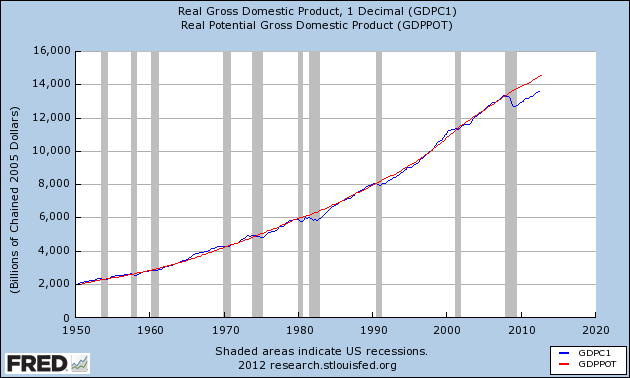
\includegraphics{images/GDP-POT-fredgraph.png}

}

\caption{\label{fig-chart-pgdp}\textbf{Potential Output} The red graph
represents the U.S. Congressional Budget Office's estimates of potential
real GDP (in billions of chained 2000 dollars). The blue graph
represents actual real GDP. The excess of potential GDP over actual GDP
is referred to as the \textbf{GDP gap}. The gray bars in the figure
represent the periods of \textbf{recession} in the U.S. economy. Actual
GDP is typically less than potential GDP during recessions. Source: Data
on real GDP was downloaded from
\url{https://fred.stlouisfed.org/series/GDPC1} and data on potential
real GDP was downloaded from
\url{https://fred.stlouisfed.org/series/GDPPOT}, both on November 25,
2012.}

\end{figure}%

As was just mentioned, a country's real GDP is assumed to be equal to
its real potential GDP in the long run. \emph{Potential Real GDP is the
real GDP that would be produced if the utilization of the resources of
the economy were at normal
levels\index{gross domestic product!potential}}. Actual real GDP, \(Y\),
is less than potential real GDP when resources are under-utilized, as in
a recession. On the other hand, if resource utilization is at abnormally
high levels, as in a booming economy, actual real GDP could exceed
potential real GDP.

An economy's potential GDP depends on several factors. Potential GDP
will be high if (a) the quantity and quality of the productive resources
that the country is endowed with are high, (b) it can purchase from
other countries at a low price the resources it does not have, (c) it
has access to advanced technology, and (d) it has the economic policies
and cultural institutions that encourage the efficient utilization of
all resources. However, for the purposes of this book, \(Y^p\) will be
regarded as exogenous, something as inscrutable as the weather.

The Congressional Budget Office, an arm of the United States Congress,
publishes estimates of America's potential real GDP.\footnote{For
  details, see \emph{CBO's Method for Estimating Potential Output: An
  Update}, Congressional Budget Office, August 2001,
  \url{https://www.cbo.gov/sites/default/files/107th-congress-2001-2002/reports/potentialoutput.pdf}
  and \textcite{shackleton2018estimating}
  (\href{https://www.cbo.gov/publication/53558}{online}).} Potential GDP
is a conceptual notion that cannot be directly observed. But that does
not mean that it cannot be reliably estimated. See figure
Figure~\ref{fig-chart-pgdp} for a look at the CBO's estimates of
America's potential real GDP.

\section{What Is Short-Run Analysis?}\label{sec-shortana}

In short-run analysis\index{macroeconomic analysis!short-run analysis} I
make the following simplifying assumptions:

\begin{itemize}
\tightlist
\item
  \textbf{Fixed Prices} \index{prices, fixed in the short run}: The
  variables \(P\), \(P^*\) are assumed to be exogenous and constant.
\item
  \textbf{Long-Run Expectations}
  \index{expectations!anchored to the long run}: People's expectations
  about the future value of a variable (that is, variables such as
  \(E^e_f\) and \(E^e_g\)) are assumed to be equal to its long-run
  value. For example, if \(E_{fLR}\) represents the value of the foreign
  country's currency in long-run equilibrium, then \(E^e_f=E_{fLR}\) is
  assumed true in the short run.
\end{itemize}

The assumptions about expectations formation for the long and short runs
can, therefore, be combined into one simple statement: \(E^e_f=E_{fLR}\)
irrespective of whether we are doing long-run analysis or short-run
analysis.

\bookmarksetup{startatroot}

\chapter{Exchange Rate Systems: Fixed and Flexible}\label{sec-exchsys}

We saw in Chapter~\ref{sec-basicequations} that our theory of
international macroeconomics has three equations representing
equilibrium in the markets for goods, money, and foreign exchange. We
saw in Chapter~\ref{sec-theqvar} that for such a theory to be useful,
exactly three of the many variables in our three equations must be
endogenous, and the rest exogenous. And we saw in
Chapter~\ref{sec-shortlong} that the classification of our variables
into endogenous and exogenous groups depends on (a) whether we are doing
long-run analysis or short-run analysis and (b) whether we are
considering a country with flexible or fixed exchange rates. This
chapter focuses on exchange rate systems and the way international
macroeconomic theory adapts to the exchange rate system being
considered.

\section{When Is a Country Said to Have a Fixed Exchange Rate
System?}\label{sec-fixexrates}

A country is said to have a fixed exchange rate
system\index{exchange rate!fixed} if its central bank (such as the
Federal Reserve in the US or the Bank of Japan in, you guessed it,
Japan) chooses a value for the nominal exchange rate (\(E\)) and
announces that it is ready and willing to buy and/or sell any amount of
the domestic currency at the rate of \(E\) units of the domestic
currency for one unit of the foreign currency. This action effectively
fixes \(E\) at the central bank's chosen
value.\index{central banks!control of exchange rates}

\begin{figure}

\centering{

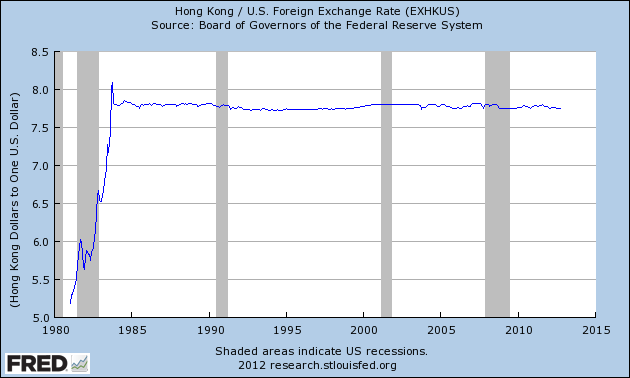
\includegraphics{images/HKdollar-fredgraph.png}

}

\caption{\label{fig-chart-hong-kong-dollar}Here's an example of a fixed
exchange rate. Notice that the Hong Kong dollar is fixed at about 7.80
Hong Kong dollars per U.S. dollar. Source:
\url{https://fred.stlouisfed.org/series/EXHKUS}, downloaded on November
25, 2012.}

\end{figure}%

To see how this works, let us talk not about currencies but about
something completely different: let us talk about wheat! Assume that
Bill Gates announces that he is willing to buy and/or sell any amount of
wheat for \$15 a bushel.\footnote{Let's assume that Bill has a large
  stock of wheat and a large amount of money so as to be able to deliver
  on his promise.} It is then straightforward to show that the market
price will quickly become \$15 per bushel. To see why, suppose the price
was \$18 per bushel before Bill's announcement. As soon as Bill makes
his announcement, wheat \emph{buyers}, who quite understandably prefer
the \$15 price to the \$18 price, would rush to buy Bill's wheat at \$15
per bushel and, as a result, all other wheat sellers would soon be
forced to sell at Bill's price. If, on the other hand, the price was
\$12 before Bill's announcement, all \emph{sellers} would sell their
wheat to Bill unless other buyers start paying \$15 as well. In short,
the price of wheat will become whatever Bill wants it to be.

In the same way, the central bank of a nation can fix the nominal
exchange rate of the domestic currency if it starts buying and selling
the currency at some chosen price.

\subsection{Money Supply Under Fixed Exchange
Rates}\label{sec-fixexrates-money}

Here, the important point to note is that \emph{under a fixed exchange
rate system the central bank loses all control over \(M\), the country's
money supply}.\index{central banks!control of money supply} To see why,
suppose the US Federal Reserve announces that it will buy and/or sell
dollars at 1.50 euros per dollar. If people rush to buy dollars from the
Fed at that price, the Fed will have to print a fresh batch of dollars
and pretty soon all those newly printed dollar bills will end up in the
wallets of those who traded in their euros. That is, the US money supply
(\(M\)), which, you may recall from Section~\ref{sec-msupply}, is the
currency \emph{held by the public} plus the value of their checking
accounts, will increase. Similarly, if people choose to sell their
dollars to the Fed in exchange for British pounds, the US money supply
(\(M\)) will decrease because the dollars sold to the Fed are longer in
peoples' wallets. In short, the money supply will be whatever the people
want it to be and not necessarily what the Federal Reserve wants it to
be.

In other words, \(M\), \emph{the money supply, becomes an endogenous
variable}. That is, \(M\) will become a variable whose up and down
movements our theory will have to explain. Just as \(Y\), \(C\), \(EX\),
\(IM\), etc. are variables whose movements our theory will have to
predict, \(M\) will also be a variable whose movements our theory will
have to predict.

To sum up, for the analysis of a fixed exchange rate system \(E\) will
be regarded as exogenous and constant---that is, \(E_f=E\), which
implies that \(E_g\) is not just exogenous, it is zero---and \(M\) will
be regarded as endogenous.\footnote{Since \(M\) is endogenous, so is
  \(M_g\), the growth rate of \(M\). \(M_g\) will play a role in
  Chapter~\ref{sec-longnom}, which is about long-run analysis.}

\begin{figure}

\centering{

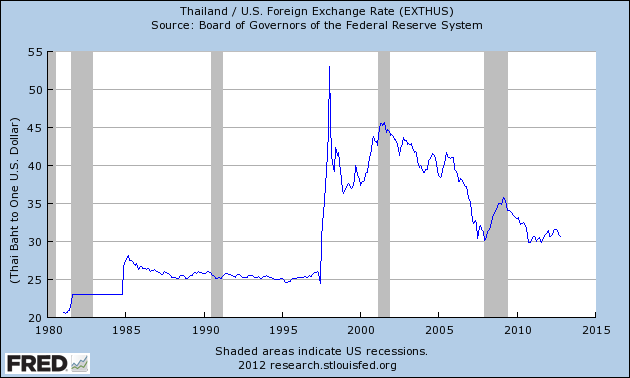
\includegraphics{images/baht-fredgraph.png}

}

\caption{\label{fig-chart-thai-baht}Here's an example of a fixed
exchange rate system that turned into a flexible exchange rate system.
For about a decade until July 2, 1997, the Thai baht was pegged at about
25 to the dollar. But a currency crisis developed in 1997 and it became
impossible for the central bank of Thailand to continue to keep its
obligation to pay one U.S. dollar to whoever offered 25 baht in payment.
At that point the baht became a flexible (or, floating) currency. It
rapidly lost value---note the sharp spike in the chart---reaching the
low-point of 53 baht per dollar in January 1998. Although the baht has
gradually regained some of its lost value it has still not reached its
pre-crisis value of 25 baht per U.S. dollar. There will be more on
currency crises in a later chapter. Source:
\url{https://fred.stlouisfed.org/series/EXTHUS}, downloaded on November
25, 2012.}

\end{figure}%

\section{When Is a Country Said to Have a Flexible Exchange Rate
System?}\label{sec-flexexrates}

A country is said to have a flexible exchange rate
system\index{exchange rate!flexible} if the exchange rate (\(E\)) is
determined in the foreign exchange market without any significant
intervention or manipulation by its central bank.\footnote{For more on
  \(E\), see Section~\ref{sec-nomexrates}.} And since, in this case, the
central bank does not make any promises to buy and/or sell the domestic
currency at some fixed price, it can control the amount of the domestic
currency that is circulating in private hands. Money supply, \(M\),
therefore, becomes whatever the central bank wants it to be. In other
words, \(M\) becomes an exogenous
variable.\index{central banks!control of money supply}

To sum up, the analysis of flexible exchange rate systems regards \(E\)
as endogenous and \(M\) as exogenous.\footnote{\(M_g\), the growth rate
  of \(M\), will, therefore, also be exogenous. As was mentioned
  earlier, \(M_g\) will play a role in Chapter~\ref{sec-longnom}, which
  is about long-run analysis.}

\begin{figure}

\centering{

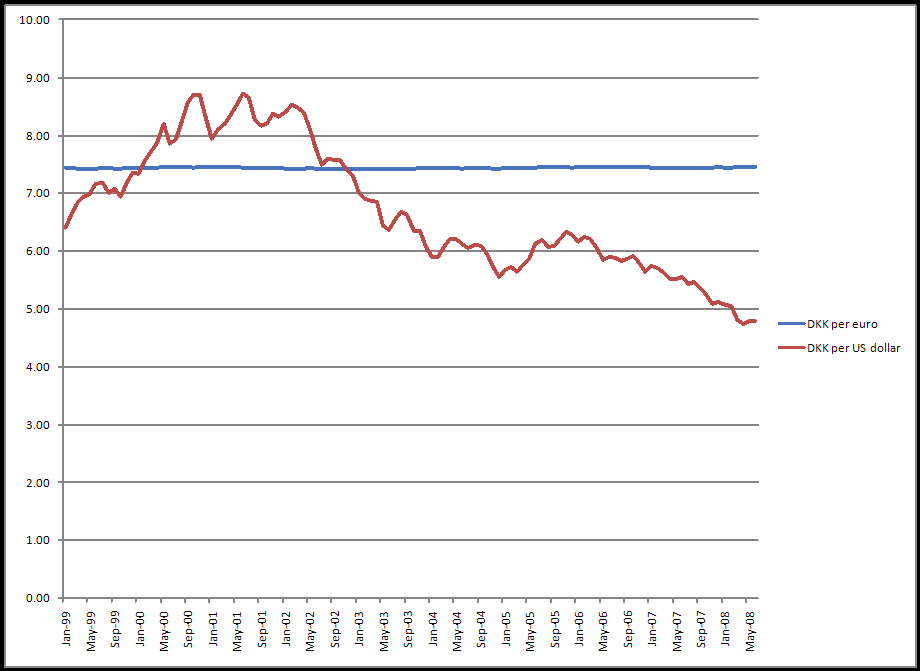
\includegraphics{images/DKK.png}

}

\caption{\label{fig-chart-danish-kroner}The Danish Kroner appears to
float freely with respect to the U.S. dollar. But Denmark actually has a
fixed exchange rate system, with its exchange rate set at about 7.45
Kroner per Euro. Source: \url{https://www.nationalbanken.dk/en},
downloaded on July 6, 2008.}

\end{figure}%

\bookmarksetup{startatroot}

\chapter{Long-Run Predictions: The Real World}\label{sec-longreal}

What would be the long-run (or, eventual) consequence of an increase in
taxes? This and similar other questions are discussed in this chapter
and the next. These questions will all have the same format: If there is
a permanent increase in {[}insert the name of an exogenous variable{]},
what will happen in the long run to {[}insert the name of an endogenous
variable{]}? Notice that the focus will always be on prediction, because
only when a theory takes a stand by making a prediction can it be tested
with actual data.

We have seen the distinctions between nominal and real gross domestic
product--- in Chapter~\ref{sec-niaccounts} --- and nominal and real
exchange rates---in Chapter~\ref{sec-exrates}. Nominal variables are not
adjusted for inflation, whereas real variables are. Real variables could
meaningfully describe even a barter economy in which money does not
exist. Nominal variables, on the other hand, would make sense only in
monetary economies. This chapter focuses on the long-run effects of
exogenous variables on \emph{real} endogenous variables. The next
chapter takes on nominal endogenous variables, such as the price level,
the inflation rate, and the nominal exchange rate.

As I said in Section~\ref{sec-longana}, for long-run
analysis\index{macroeconomic analysis!long-run analysis} I will assume:

\begin{itemize}
\tightlist
\item
  Full Employment\index{full employment}---i.e., \(Y = Y^p\)---and
\item
  Perfect Foresight\index{perfect foresight}---i.e., \(E^e_f=E_f\).
\end{itemize}

\section{Gross Domestic Product}\label{sec-longy}

Recall from Section~\ref{sec-exoendo} that \(Y^p\), potential GDP, is,
for us, an exogenous variable. Therefore, the full-employment
assumption, \(Y=Y^p\), says all that can be said about the long-run
behavior of GDP: \emph{\(Y\) is equal to \(Y^p\) and unaffected by all
other exogenous variables.} This is shown in the \(Y\)-column of
Table~\ref{tbl-real_long}, which shows the ceteris paribus effects of
each exogenous variable on all endogenous variables.\footnote{See
  Section~\ref{sec-whytheory} for the definition of ceteris paribus
  effects.}

\section{Consumption}\label{sec-longc}

Recall from Equation~\ref{eq-consfn} in Section~\ref{sec-consumption}
that consumption (\(C\)) is directly related to disposable income
(\(Y-T\)) as in the consumption function, \(C=C(Y-T)\). The
full-employment assumption that we just saw then implies

\begin{equation}\phantomsection\label{eq-longc}{
C=C(Y^p-T).
}\end{equation} As \(T\) and \(Y^p\) are assumed exogenous for our
purposes---see Section~\ref{sec-exoendo} ---we can say right here all
that can be said about the long-run behavior of consumption: \emph{\(C\)
is directly affected by \(Y^p\), inversely affected by \(T\), and
unaffected by all other exogenous variables}. These are ceteris paribus
effects, and they are shown in the \(C\)-column of
Table~\ref{tbl-real_long}.

As consumption is an endogenous variable, we need to be able to explain
the ups and downs of \(C\). Once we have succeeded in expressing an
endogenous variable in terms of exogenous variables alone---as we have
done in Equation~\ref{eq-longc} ---we can't go any further because, by
definition, exogenous variables are variables we know nothing about
(except that they may help explain the up and down movements of our
endogenous variables). We don't know what makes \(Y^p\) and \(T\)
fluctuate. Therefore, once we have expressed \(C\) entirely in terms of
\(Y^p\) and \(T\), we cannot say anything more about \(C\).

\section{Net Exports}\label{sec-longnx}

Recall from Equation~\ref{eq-IS} that \(Y=C+I+G+NX\) is the condition
that must be satisfied for the goods market to be in equilibrium.
Therefore, \begin{equation}\phantomsection\label{eq-longnx}{
\begin{eqnarray}
NX&=&Y-C(Y-T)-I-G\nonumber \\
&=&Y^p-C(Y^p-T)-I-G
\end{eqnarray}
}\end{equation} in long-run equilibrium.

Notice that all the variables on the right hand side of this equation
are exogenous. Therefore this equation tells us all that can be said
about the long run behavior of \(NX\).

For example, what if there is a permanent increase in either \(I\) or
\(G\) or both? It follows directly from Equation~\ref{eq-longnx} that
\(NX\) will decrease.

If, however, you are persuaded by the logic of Ricardian equivalence,
which we saw in Section~\ref{sec-mpc}, then the analysis would be a lot
more subtle. Suppose \(G\) has permanently increased by \$100 a year.
Section~\ref{sec-mpc} implies that even though the government in this
case has not raised taxes to pay for the increased spending, people may
behave as if taxes have gone up by the same \$100. In that case, \(C\)
would fall. For a \$100 increase in government spending that is
perceived to be permanent, \(C\) would also fall by \$100, the full
extent of the perceived/feared increase in \(T\) and the actual increase
in \(G\). And, therefore, the decline in \(C\) would cancel out the
increase in \(G\) in Equation~\ref{eq-longnx}, leaving \(NX\) unchanged.

The effect of an increase in taxes is equally easy to figure out. When
\(T\) increases, \(C\) decreases, as we saw in Section~\ref{sec-longc}
above. Therefore, by Equation~\ref{eq-longnx}, \(NX\) will increase.

Finally, what if there is a permanent increase in the domestic country's
potential real GDP (\(Y^p\)) by, say, \$1.00? Consumption spending will
increase---as we saw in Section~\ref{sec-consumption} above---by the
magnitude of the marginal propensity to consume (MPC). And, as we saw in
Section~\ref{sec-mpc}, the size of the MPC depends on whether the change
in income is perceived to be permanent or temporary. Specifically, if
the one-dollar increase in income is perceived to be permanent, \(C\)
will also rise by one dollar and therefore, by Equation~\ref{eq-longnx},
\(NX\) will be \emph{unchanged}. But when the one-dollar increase in
income is perceived to be less than permanent, \(C\) will rise by a
fraction of one dollar. So, \(Y^p-C(Y^p-T)\) will increase. Therefore,
by Equation~\ref{eq-longnx}, \(NX\) will be \emph{increase}.

So, what's one to believe? If the permanent increase in \(Y^p\) is
perceived to be permanent, \(NX\) is unaffected by the increase in
\(Y^p\). But if people doubt the permanence of this increase in \(Y^p\),
\(NX\) increases. It makes sense to split the difference and say that
when potential real GDP increases, so does net exports, because in
actual cases there may be no increase in potential real GDP that is
perceived to be entirely permanent.

To sum up, what does our analysis say about the long-run behavior of a
country's trade balance or net exports? \emph{A country's net exports is
directly affected by its potential real GDP and its tax revenues;
inversely affected by government spending and investment spending; and
unaffected by all other exogenous variables}. These are ceteris paribus
effects, and they are shown in the \(NX\)-column of
Table~\ref{tbl-real_long}.

\subsection{Policies to raise net exports}\label{sec-boost-nx}

The important lesson of our analysis is that the only dependable way to
achieve a long-run increase in net exports is through `fiscal austerity'
or `belt tightening' by the country's government. When government
spending is reduced (\(G\downarrow\)) and/or taxes are raised
(\(T\uparrow\)), net exports increases (\(NX\uparrow\)).

A surprising related point in that \textbf{tariffs}, which are taxes
imposed only on imported goods and services, and other protectionist
policies cannot affect a country's net exports.\index{tariffs} It would
be hard to make a cogent argument that tariffs would lead to an increase
in \(Y^p\) or in \(Y^p-C(Y^p-T)\), or to a decrease in \(I\) or in
\(G\). Therefore, it would be hard to make a persuasive argument that
\(NX=Y^p-C(Y^p-T)-I-G\) would increase in the long run if tariffs or
other protectionist measures are implemented.

\section{Real Exchange Rate}\label{sec-longq}

The analysis of the long-run behavior of the real exchange rate (\(q\))
depends on whether or not the law of one price is assumed to be
true.\footnote{See Section~\ref{sec-realexrates} for more on the real
  exchange rate, and Section~\ref{sec-summary-nxp} and
  Section~\ref{sec-appp} for more on the law of one price.}

\subsection{Under absolute purchasing power
parity}\label{sec-q-long-appp}

\index{purchasing power parity!absolute}

Recall from Section~\ref{sec-appp} that under the law of one
price---also called absolute purchasing power parity---the real exchange
rate must always be \(q=1\) and the relation between net exports and the
real exchange rate is represented by a horizontal net exports curve such
as the one shown in the right panel of
Figure~\ref{fig-net_exports_general}. In this case, the analysis of the
long-run behavior of the real exchange rate is trivial: it will always
stay at \(q=1\), nothing can make it budge.

Let us, therefore, move on to the less restrictive case shown by the
rising net exports curve in the left panel of
Figure~\ref{fig-net_exports_general}.

\begin{figure}

\centering{

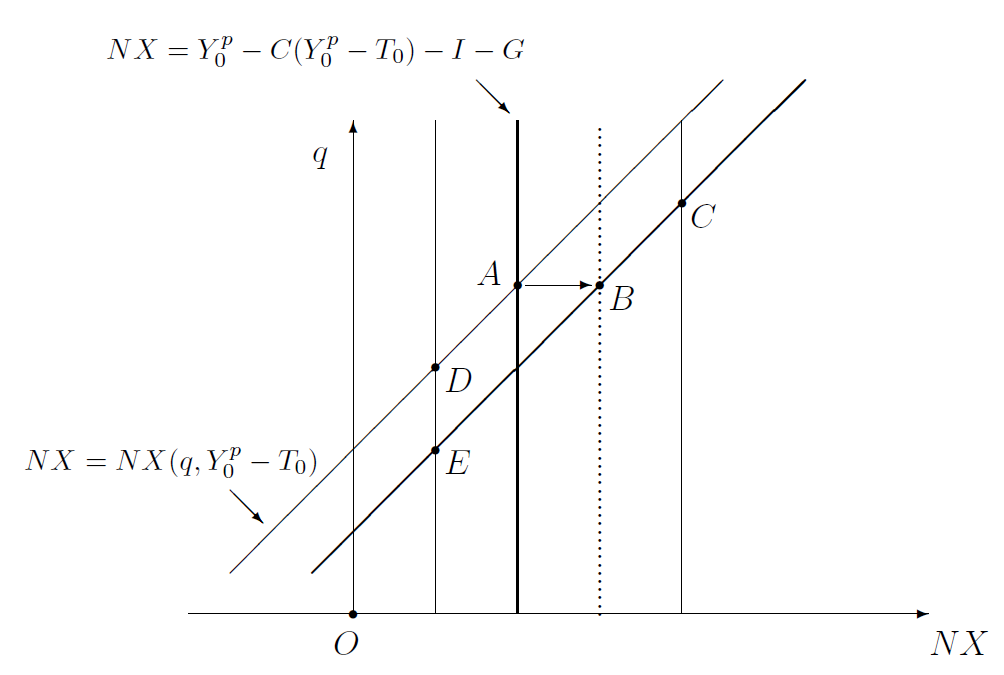
\includegraphics{images/NX_real_exch_rate_LR_eqm.png}

}

\caption{\label{fig-NX_real_exch_rate_LR_eqm}This diagram shows how real
exchange rates can change. In long-run equilibrium, both
\(NX=NX(q,Y^p-T)\) and \(NX=Y^p-C(Y^p-T)-I-G\) must be true. Therefore,
for the initial values \(Y^p=Y^p_0\) and \(T=T_0\), the equilibrium is
at point \(A\). When either \(T\) increases or \(Y^p\) decreases, the
upward-sloping net exports curve shifts right, as shown. When \(T\)
increases, the vertical net exports curve also shifts right, but by more
than the upward-sloping net exports curve does. As a result, the long
run equilibrium moves from \(A\) to \(C\). This implies a direct effect
of \(T\) on \(q\). When \(Y^p\) decreases, the vertical net exports
curve shifts left. As a result, the long run equilibrium moves from
\(A\) to \(E\). This implies a direct effect of \(Y^p\) on \(q\); they
both move in the same direction. When either \(I\) or \(G\) increases,
the upward-sloping net exports curve is unaffected and the vertical net
exports curve shifts left, taking the equilibrium from \(A\) to \(D\).
This shows that \(I\) and \(G\) have inverse effects on \(q\). No other
exogenous variable affects \(q\). (Note that absolute purchasing power
parity has \emph{not} been assumed.)}

\end{figure}%

\subsection{Without absolute purchasing power
parity}\label{sec-q-long-no-appp}

\subsubsection{Two net exports curves: one upward-sloping, the other
vertical}\label{sec-nx-curves}

Recall from Equation~\ref{eq-netexports} that \(NX=NX(q,Y-T)\) is
directly related to \(q\) and inversely related to \(Y-T\). For some
given value of \(Y-T\), the direct effect of \(q\) on \(NX\) is shown as
an \emph{upward-sloping net exports curve} in the left panels of
Figure~\ref{fig-net_exports_general} and
Figure~\ref{fig-net_exports_real_exchange_rate} and yet again in
Figure~\ref{fig-NX_real_exch_rate_LR_eqm} in this chapter.\footnote{Figure~\ref{fig-NX_real_exch_rate_LR_eqm}
  also makes use of the long-run assumption of \(Y=Y^p\). The
  upward-rising net exports curve marked with a label and an arrow
  assumes that the magnitude of potential output is \(Y^p=Y^p_0\) and
  the magnitude of taxes is \(T=T_0\).}

These figures also show that a decrease in \(Y^p\) or an increase in
\(T\) or, generally, \emph{a decrease in \(Y-T=Y^p-T\) shifts the
upward-sloping net exports curve downward or to the right}. A poorer
country imports less and, therefore, sees its net exports increase at
any given value of the real exchange rate.

In fact, we can be more specific about the size of this shift. Recall
from Section~\ref{sec-imports} that if \(Y-T\) decreases by a dollar,
both consumption (\(C\)) and imports (\(IM\)) will decrease, but the
latter will decrease less than the former. In particular, \(C\)
decreases by the marginal propensity to consume (MPC) and \(IM\)
decreases by less than the MPC. It therefore follows that when \(Y^p-T\)
decreases by a dollar, \(NX\) will increase by less than the MPC, at any
given value of the real exchange rate. In other words, \emph{when
\(Y^p-T\) decreases by a dollar, the vertical net exports curve shifts
right by a length smaller than the MPC}.

Now, as we saw in Section~\ref{sec-longnx} above, the goods market's
equilibrium condition, \(Y=C+I+G+NX\), also tells us something about a
country's net exports. Specifically, \(NX=Y-C(Y-T)-I-G\) or, in long-run
equilibrium, \(NX=Y^p-C(Y^p-T)-I-G\). As this equation expresses \(NX\)
as entirely independent of \(q\), it can be graphically shown as the
\emph{vertical net exports curve} in
Figure~\ref{fig-NX_real_exch_rate_LR_eqm}. It is vertical because
changes in \(q\) have no effect on \(NX=Y^p-C(Y^p-T)-I-G\). Of course,
if \(Y^p\) or \(T\) or \(I\) or \(G\) changes in value, so will \(NX\)
and the vertical net exports curve will shift.

For example, \emph{if either \(I\) or \(G\) increases by a dollar,
\(NX=Y^p-C(Y^p-T)-I-G\) will decrease by a dollar and the vertical net
exports curve will shift left by a dollar}. If \(T\) increases by a
dollar, \(C\) will decrease, not by the entire dollar's increase in
taxes but by a fraction---a fraction that was called the marginal
propensity to consume (MPC) in Section~\ref{sec-mpc}. As a result,
\(NX=Y^p-C(Y^p-T)-I-G\) will increase by that same amount (the MPC).
Therefore, \emph{when \(T\) increases by a dollar, the vertical net
exports curve shifts right by a length equal to the MPC}.

Finally, if \(Y^p\) increases by a dollar, then \(C(Y^p-T)\) increases
by the MPC. Therefore, \(Y^p-C(Y^p-T)\), which is simply the part of
total income that is saved, will increase by \(1-\text{MPC}\) dollars,
which is equivalent to MPS dollars, where MPS stands for the marginal
propensity to save---see Section~\ref{sec-mpc}. In short, \emph{when
\(Y^p\) increases by a dollar, the vertical net exports curve shifts
right by MPS dollars}.

\subsubsection{Equilibrium}\label{sec-eqm-no-appp}

Now, in long-run equilibrium, what we know about the factors that
influence net exports (\(NX=NX(q,Y^p-T)\), the upward-sloping net
exports curve) must be consistent with what the goods market's
equilibrium condition tells us about net exports
(\(NX=Y^p-C(Y^p-T)-I-G\), the vertical net exports curve). Therefore, in
Figure~\ref{fig-NX_real_exch_rate_LR_eqm}, the long-run equilibrium must
be at \(A\), where the two net exports curves intersect. This pinpoints
the long-run equilibrium level of the real exchange rate.

And, as we know how the two net exports curve shift when there are
changes in the magnitudes of the exogenous variables \(Y^p\), \(T\),
\(I\), and \(G\), we will be able to predict how the real exchange rate
is affected by these changes.

For example, as we saw in the previous section, if either \(I\) or \(G\)
increases, the upward-sloping net exports curve is unaffected and the
vertical net exports curve shifts left. Therefore, the long-run
equilibrium in Figure~\ref{fig-NX_real_exch_rate_LR_eqm} moves from
\(A\) to \(D\), implying a decrease in \(q\). That is, \emph{increases
in domestic spending either by businesses (\(I\uparrow\)) or the
government (\(G\uparrow\)) boosts the relative demand for the domestic
country's products and thereby raises the relative price of those
products or, equivalently, reduces the relative price of foreign goods
(\(q\downarrow\))}.

We have also seen that if \(T\) increases by a dollar, the
upward-sloping net exports curve shifts right by \emph{less than} the
MPC. On the other hand, we have also seen that the vertical net exports
curve shifts right by a length \emph{equal to} the MPC. Therefore, the
long-run equilibrium in Figure~\ref{fig-NX_real_exch_rate_LR_eqm} will
move from \(A\) to \(C\), implying an increase in \(q\). That is,
\emph{an increase in taxes (\(T\uparrow\)) leads to a higher real
exchange rate (\(q\uparrow\))}. This is intuitive: A rise in taxes
squeezes domestic consumption, which reduces demand in the domestic
economy. This reduces the relative price of domestic goods or,
equivalently, raises the relative price of foreign-made goods, which is
the real exchange rate.

Finally, we have seen in the previous section that if \(Y^p\) decreases
by a dollar, the upward-sloping net exports curve shifts right and the
vertical net exports curve shifts left. Therefore, the long-run
equilibrium in Figure~\ref{fig-NX_real_exch_rate_LR_eqm} moves from
\(A\) to \(E\), implying a decrease in \(q\). That is, as in the case of
\(T\), \emph{a change in \(Y^p\) brings about a change in \(q\) in the
same direction}.

And, again, this is intuitive. If a country becomes more productive
(\(Y^p\uparrow\)) its goods become relatively more plentiful in the
world economy. This drives down the relative price of domestic goods or,
equivalently, makes foreign-made goods relatively more expensive
(\(q\uparrow\)).

\subsubsection{Real Exchange Rate:
Summary}\label{sec-real-ex-rates-summary}

To summarize, under absolute purchasing power parity, \(q=1\) in all
situations and is, therefore, unaffected by changes in our exogenous
variables. When absolute purchasing power parity is not applicable,
\emph{in long run equilibrium, the real exchange rate (\(q\)) is
inversely affected by government spending (\(G\)) and business
investment (\(I\)); directly affected by taxes (\(T\)) and potential
output (\(Y^p\)); and unaffected by all other exogenous variables}.
These ceteris paribus effects are shown in the \(q\)-column of
Table~\ref{tbl-real_long}.

In Chapter~\ref{sec-longnom}, a less stringent version of absolute
purchasing power parity---called \emph{relative} purchasing power
parity---is assumed.\index{purchasing power parity!relative} Relative
purchasing power parity is the assumption that the real exchange rate is
\emph{constant} over time, though not necessarily equal to one---see
Section~\ref{sec-rppp}. Given the results summarized in the previous
paragraph, for the real exchange rate to be constant, either \(I\),
\(G\), \(T\), and \(Y^p\) would have to be constant or---and this is an
unlikely possibility---they would have to change in concert in such a
way that they cancel each others' effects on \(q\) and, therefore, leave
the real exchange rate constant.

\begin{table}

\caption{\label{tbl-real_long}\textbf{Macroeconomic Behavior of Real
Variables in the Long Run}. All variables named in the first column are
exogenous and all variables listed in the first row are endogenous. Each
cell in the table shows the relation between the exogenous variable and
the endogenous variable aligned with the cell. The +/?/- symbols denote
a direct/ambiguous/inverse relation. A blank cell denotes that there is
no relation. Note that absolute purchasing power parity has *not been
assumed. Under APPP, the last three columns would be gone and the rest
of the table would be unaffected. Recall that \(q\) is constant at
\(q=1\) under APPP. Moreover, the \(EX\) and \(IM\) columns would be
gone too, as they would no longer make sense, being infinitely elastic
at \(q=1\).}

\centering{

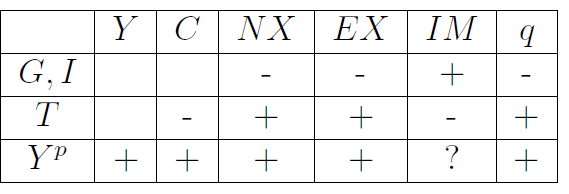
\includegraphics{images/real_long.png}

}

\end{table}%

\section{Exports}\label{sec-longexp}

Recall from Equation~\ref{eq-exp} in Section~\ref{sec-exports} that the
amount of domestically produced goods that is exported (\(EX=EX(q)\)),
is directly related to the real exchange rate (\(q\)).\footnote{For a
  recap on real exchange rates, see Section~\ref{sec-realexrates}.}

Therefore, if an exogenous variable has a direct/non-existent/inverse
effect on \(q\) it will have an identical effect on \(EX\). In
Table~\ref{tbl-real_long}, therefore, the \(EX\)-column must necessarily
be the same as the \(q\)-column that was discussed in
Section~\ref{sec-longq} above.

\section{Imports}\label{sec-longimp}

Recall from Equation~\ref{eq-imports} in Section~\ref{sec-imports} that
the amount imported by a country in the long run (\(IM=IM(q,Y^p-T)\)) is
inversely related to the real exchange rate (\(q\)) and directly related
to the disposable potential real GDP (\(Y^p-T\)).

According to Section~\ref{sec-longq}, a ceteris paribus increase in
\(G\) or \(I\) causes a decrease \(q\). This, in turn, would increase
\(IM\).

An increase in \(Y^p\) leads to a higher \(q\), which reduces imports,
and a higher \(Y^p-T\), which increases imports. Therefore, the overall
effect of \(Y^p\) on \(IM\) is ambiguous.

An increase in \(T\) leads to an increase in \(q\) and a decrease in
\(Y^p-T\). Both lead to reduced imports.

To summarize, \emph{imports are directly affected by \(G\) and \(I\);
inversely affected by \(T\); ambiguously affected by \(Y^p\); and
unaffected by all other exogenous variables}.

\section{Macroeconomic Behavior of Real Variables in the Long Run:
Conclusions}\label{sec-longrealconclusions}

We have been discussing the long-run effects of our exogenous variables
on our real endogenous variables. The results are summarized in
Table~\ref{tbl-real_long}.

Note that only fiscal policy can affect net exports; tariffs, for
example, are useless. Contractionary fiscal policy---i.e., either a cut
in government spending, \(G\), or an increase in taxes, \(T\), or
both---can reliably increase net
exports.\index{policy!fiscal policy!contractionary}

Note also that neither monetary variables---such as \(M\), \(P\), and
\(E\)---nor the money market equilibrium condition---that is
\(M=L(R)\cdot P\cdot Y\) in Section~\ref{sec-summary-moneyeqm} ---played
any role in this chapter's discussion of the long run behavior of real
variables. In fact, I did not even mention any monetary variables before
this paragraph. This is an instance of an idea with a long pedigree in
economics called \emph{monetary neutrality}: any change in the quantity
of money in circulation (\(M\)) will not affect a real variable.

While monetary neutrality is thought to be a good description of an
economy in the long run, we will see that things are different in the
short run. In the short run, \(M\) can be an important determinant of
real variables such as \(Y\), \(C\), \(I\), \(q\), and \(NX\).

Note, finally, that in this chapter I did not bring up the issue of
whether the country has a flexible exchange rate system or a fixed
exchange rate system. In other words, the exchange rate system has
nothing to do with the long run behavior of real variables. Put yet
another way, the long run analysis of real variables will have nothing
useful to say if a country is debating what kind of exchange rate system
to adopt: both systems have the same real consequences.

\bookmarksetup{startatroot}

\chapter{Long-Run Predictions: The Nominal World}\label{sec-longnom}

This chapter continues the discussion of long-run equilibrium that I
began in the last chapter. That chapter had focused on \textbf{real
variables} \index{variables!real}, which are variables that would be
meaningful even in a discussion of a barter-based world in which nobody
uses cash as well as a world in which people use cash. This chapter
focuses on \textbf{nominal variables} \index{variables!nominal}, such as
the nominal exchange rate and the rate of inflation, which mean
something only in an economy in which people use money.

\section{The Classical Dichotomy and Monetary
Neutrality}\label{sec-monneutral}

The notion that it is theoretically useful to classify economic
variables into real and nominal variables is called the
\textbf{classical dichotomy} \index{classical dichotomy}. The related
idea that real and nominal variables can be discussed separately because
changes in \(M\), the quantity of money, do not affect real variables,
is called \textbf{monetary neutrality}
\index{monetary neutrality}.\footnote{The ``classical'' in classical
  dichotomy refers to the \textbf{classical school}
  \index{classical school} of economic thought that was dominant in the
  eighteenth and nineteenth centuries. Prominent representatives of the
  classical school include
  \href{https://en.wikipedia.org/wiki/David_Hume}{David Hume}
  (1711--1776), \href{https://en.wikipedia.org/wiki/Adam_Smith}{Adam
  Smith} (1723--1790),
  \href{https://en.wikipedia.org/wiki/Thomas_Robert_Malthus}{Thomas
  Malthus} (1766--1834),
  \href{https://en.wikipedia.org/wiki/David_Ricardo}{David Ricardo}
  (1772--1823), and
  \href{https://en.wikipedia.org/wiki/John_Stuart_Mill}{John Stuart
  Mill} (1806--1873). The classical dichotomy and the theory of monetary
  neutrality were central ideas of the classical school and are
  generally attributed to Hume, although hints of these ideas have been
  found even in the writings of medieval scholars.}

The neutrality of money in the long run made it possible for me to limit
Chapter~\ref{sec-longreal} to a discussion of only the real variables.
We will see in this chapter, however, that although real variables can
be discussed without mentioning nominal variables, the reverse is not
true: changes in real exogenous variables can affect nominal endogenous
variables.

Classical economists were aware---as are today's economists---that
monetary neutrality made sense in the long run but not in the short run.
As later chapters will show, any discussion of short-run international
macroeconomics must juggle real and nominal variables simultaneously.

\section{Some Math Results on Growth Rates}\label{sec-lmath}

Before we can tackle the long-run behavior of nominal endogenous
variables, we need to do some math.

Recall from Section~\ref{sec-notngrowth} that the growth rate of a
variable is denoted here by the symbol for that variable with the letter
\(g\) attached as a subscript. It can then be shown that:

\begin{theorem}[Growth rate of a product of
variables]\protect\hypertarget{thm-gprod}{}\label{thm-gprod}

If \(z=x\cdot y\), then \(z_g=x_g+y_g\). That is, the growth rate of the
product of a bunch of variables is equal to the sum of the growth rates
of those variables.

\end{theorem}

Suppose the number of families in your town increases from 100 to 110, a
10\% increase. Suppose the average number of people per family increases
from 5 to 6, a 20\% increase. Therefore, the population of your town,
which is given by the product of the number of families and the average
family size, increases from 500 to 660, a 32\% increase. Note that 32 is
approximately equal to \(20+10=30\), the answer you'd get if you
followed Theorem~\ref{thm-gprod}.

Suppose instead that the number of families decreases from 100 to 90, a
10\% decrease or, equivalently, a \(-10\)\% \emph{in}crease. In this
case, the total population increases from 500 to 540, an 8\% increase.
Again, note that 8 is approximately equal to \(20+(-10)=10\), the answer
according to Theorem~\ref{thm-gprod}.\footnote{In case you are wondering
  where's Theorem~\ref{thm-eqnno}, please see
  Section~\ref{sec-howmanyeq}.}

A related result can also be proved:

\begin{theorem}[Growth rate of a ratio of
variables]\protect\hypertarget{thm-gratio}{}\label{thm-gratio}

If \(z=x/y\), then \(z_g=x_g-y_g\). That is, the growth rate of the
ratio of a pair of variables is equal to the growth rate of the variable
in the numerator minus the growth rate of the variable in the
denominator.

\end{theorem}

\section{Changes in the Real Exchange Rate}\label{sec-longqg}

Recall from Equation~\ref{eq-q} that the real exchange rate is
\(q=E\cdot P^*/P\). Theorem~\ref{thm-gprod} above implies that the
growth rate of \(E\cdot P^*\) is \((E\cdot P^*)_g=E_g+P_g^*=E_g+\pi^*\),
where \(\pi^*\equiv P^*_g\) is the \textbf{foreign inflation rate}.
Theorem~\ref{thm-gratio} then implies that the growth rate of
\(q=E\cdot P^*/P\) is \(q_g=(E\cdot P^*)_g-P_g=(E\cdot P^*)_g-\pi\),
where \(\pi\equiv P_g\) is the \textbf{domestic inflation rate}. It then
follows that \begin{equation}\phantomsection\label{eq-qg}{
q_g=E_g+\pi^*-\pi.
}\end{equation}

\begin{figure}

\centering{

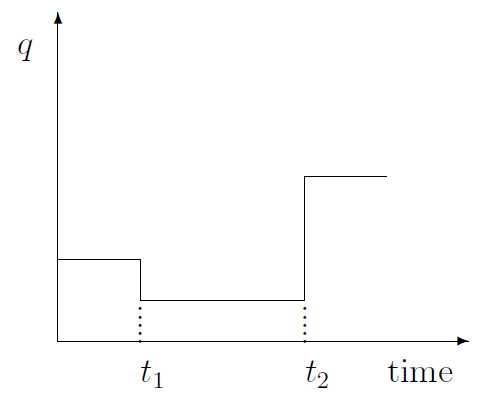
\includegraphics{images/real_exch_rate_RPPP_time.png}

}

\caption{\label{fig-q-steps}Relative Purchasing Power Parity assumes
that \(q\) is constant (\(q_g=0\)) but allows instantaneous changes in
\(q\) at isolated points in time.}

\end{figure}%

\section{Purchasing Power Parity, Absolute and Relative}\label{sec-rppp}

Recall the discussion of the law of one price---also called absolute
purchasing power parity---in Section~\ref{sec-appp}. Absolute purchasing
power parity says that \(q=1\)---see Equation~\ref{eq-absppp}. That is,
not only must the real exchange rate be constant, it must be equal to
one. The argument behind absolute purchasing power parity---which was
discussed in Section~\ref{sec-summary-nxp} ---is typically regarded as
theoretically interesting and even cogent, but factually shaky. On the
other hand, \emph{relative} purchasing power parity, a less stringent
version of the same idea, is widely accepted. Relative purchasing power
parity is the assumption that in the long run the real exchange rate
(\(q\)) is constant over time, though not necessarily equal to one.

For the rest of this chapter, I will assume relative purchasing power
parity or, equivalently,\footnote{When, in addition, I assume absolute
  purchasing power parity, I will say so explicitly.}
\begin{equation}\phantomsection\label{eq-qgLR}{
q_g=0.
}\end{equation}

Now, this may sound like a contradiction, but please hear me out. The
assumption that \(q\) is constant over time does not mean that \(q\) can
never change. Take a look at Figure~\ref{fig-q-steps}. Except for two
fleeting moments in time---\(t_1\) and \(t_2\)---\(q\) is indeed
constant. Of course \(q\) does change at \(t_1\) and \(t_2\). But these
changes are perfectly consistent with the assumption of relative
purchasing power parity.

A quick glance at the \(q\)-column of Table~\ref{tbl-real_long} will
serve as a reminder that permanent changes in \(I\), \(G\), \(T\), and
\(Y^p\) lead to long-run changes in \(q\). Therefore, my assumption that
\(q\) is constant over time except for occasional instantaneous changes
at isolated points in time, requires the additional assumption that
\(I\), \(G\), \(T\), and \(Y^p\) must be constant over time, except for
rare instantaneous changes.

\subsection{Exchange Rates: it's a race between our inflation rate and
their inflation rate}\label{sec-E-pi-race}

Equation~\ref{eq-qg} and Equation~\ref{eq-qgLR} imply something very
stark about the long-run behavior of the nominal exchange rate:

\begin{equation}\phantomsection\label{eq-eglr}{
E_g=\pi-\pi^*.
}\end{equation}

In other words, the percentage increase in the value of the foreign
currency is equal to the excess of the domestic inflation rate over the
foreign inflation rate. If US inflation is 5\% and European inflation is
3\%, then the price of one euro (measured in dollars) will rise by 2\%.
Nothing else matters. It's that simple.

\section{Uncovered Interest Parity in the Long Run}\label{sec-uiplong}

Recall, from Section~\ref{sec-summary-UIP}, that for the foreign
exchange market to be in equilibrium, uncovered interest rate parity,
\(R=R^* + E^e_g\), must be satisfied. Moreover, recall, from
Section~\ref{sec-longana}, that in long-run equilibrium expectations are
assumed to be accurate. In particular, it is assumed that \(E^e_g=E_g\).
By inserting this result and Equation~\ref{eq-eglr} into the uncovered
interest parity equation, we get
\begin{equation}\phantomsection\label{eq-nomintlong}{
R=R^* + E^e_g=R^* + E_g=R^*+\pi-\pi^*.
}\end{equation}

Recall from Section~\ref{sec-exoendo} that \(R^*\) and \(\pi^*\) are
assumed to be exogenous. I will now further assume that they are
constant, meaning that they stay unchanged at their historical levels as
the years pass by.

Consequently, one prediction from the equation above is that any change
in the domestic inflation rate (\(\pi\)) must be accompanied by an
identical change in the domestic interest rate (\(R\)). This idea is
known as the \textbf{Fisher effect}, after the economist Irving Fisher
(1867--1947).\index{Fisher effect}\index{Fisher, Irving}

Finally, I will also assume that the domestic inflation rate (\(\pi\))
is constant in the long-run equilibrium. Equation~\ref{eq-nomintlong}
then implies that the domestic nominal interest rate must be constant as
well.

\section{Money Market Equilibrium}\label{sec-moneqmlong}

Recall from Section~\ref{sec-moneyeqm} that equilibrium in the money
market can be represented by Equation~\ref{eq-LM}. The full-employment
assumption of long-run analysis---i.e., \(Y=Y^p\); see
Section~\ref{sec-longana} ---then implies:
\begin{equation}\phantomsection\label{eq-LMlong}{
M=L(R)\cdot P\cdot Y^p,
}\end{equation}

where \(L(R)\), the propensity for liquidity, is inversely related to
\(R\), the nominal interest rate.\footnote{See
  Section~\ref{sec-mdemanddet}.}

A straightforward application of Theorem~\ref{thm-gprod} of
Section~\ref{sec-lmath} to Equation~\ref{eq-LMlong} implies
\(M_g=L_g+\pi+ Y^p_g\), where \(L_g\) and \(Y^p_g\) are simply the
growth rates of \(L\) and \(Y^p\). As we saw in
Section~\ref{sec-uiplong} above, under my assumptions, \(R\) is constant
in long-run equilibrium. Therefore, \(L(R)\) must be constant too,
implying \(L_g=0\). Therefore, we get
\begin{equation}\phantomsection\label{eq-mg}{
M_g=\pi+ Y^p_g.
}\end{equation}

\section{The Economy's Growth Rate}\label{sec-ypg}

In these lectures, potential output (\(Y^p\)) and its growth rate
(\(Y^p_g\)) are assumed to be exogenous. Moreover, recall from
Section~\ref{sec-rppp}, that the assumption of relative purchasing power
parity requires the assumption that \(Y^p_g=0\).

Under absolute purchasing power parity, on the other hand, changes in
\(Y^p\) have no effect on \(q\), which is always \(q=1\) anyway.
Therefore, under absolute purchasing power parity, there is no need to
assume \(Y^p_g=0\).

\section{A Flexible Exchange Rate System}\label{sec-flex}

I will now try to describe the long-run behavior of nominal variables in
an economy that has a flexible exchange rate system.

Recall from Section~\ref{sec-flexexrates} that in a flexible exchange
rate system the nominal value of the foreign currency, \(E\), is
endogenous and the quantity of money in the domestic economy, \(M\), is
exogenous. It follows that \(E_g\), the rate of growth (or appreciation)
of the price of the foreign currency, must also be endogenous, and
\(M_g\), the growth rate of he quantity of money, must be exogenous.

\subsection{Inflation}\label{sec-pi-long-flex}

Equation~\ref{eq-mg} can be rewritten as
\begin{equation}\phantomsection\label{eq-piflex}{
\pi=M_g-Y^p_g.
}\end{equation}

Note that \(M_g\) and \(Y^p_g\) are both exogenous. Therefore, this
equation tells us all that can be said about the long-run inflation
rate: \emph{\(\pi\) is directly affected by \(M_g\), inversely affected
by \(Y^p_g\), and unaffected by all other exogenous
variables}.\footnote{This is shown in the \(\pi\)-column of
  Table~\ref{tbl-nominal_long_flex}.} In fact, the effects are
one-for-one: If the growth in the money supply speeds up by two
percentage points (or if the growth of GDP slows down by two percentage
points), inflation will speed up by the same two percentage points.

Inflation, in the long run, is a race between money supply and real GDP.
Imagine what would happen if the monetary authorities of a country
decide one day to print massive quantities of currency and drop them all
across the country from helicopters. Once they have recovered from the
initial shock, the people will rush to grab the money as fast as they
possibly can. Cash-strapped people would rush immediately to the mall to
buy stuff. Others would deposit the money in their bank accounts. But
their bank managers would, as soon as possible, lend the money out to
borrowers, because banks make money by lending their depositors' money
at interest rates that are higher than what the depositors are being
paid. So, one way or another, the helicopter money would end up in the
hands of eager shoppers. But the cruel irony is that the amount of stuff
available for people to buy has not changed; after all, the amount of
labor, land, and other productive resources did not magically increase
when the money rained down from the helicopters. Therefore, the people
will end up spending more money on the same amount of goods, which is
another way of saying that all that they will do is bid up the prices of
goods!

The amount of goods produced and purchased will remain unaffected by the
helicopter money. And, indeed, why would it? If it were possible to
increase production by simply printing money and dropping it everywhere
from helicopters, every country in the world would have easily attained
a princely standard of living. The fact that there are many poor people
and poor countries all over the world is proof that printing currency
bills cannot lead to higher output. All it does is raise prices.

Of course, \(Y^p\) could increase for other reasons, such as increases
in the labor force, the accumulation of capital equipment, technological
progress, etc. If real potential GDP increases at the annual rate of
3.5\% and the money supply increases at the rate of 5.0\%, then
Equation~\ref{eq-piflex} tells us that inflation will run at the annual
rate of \(5.0-3.5=1.5\)\%.

Note that \(Y^p_g\), a real variable, does have an effect on \(\pi\), a
nominal variable. This illustrates the point made in my discussion of
monetary neutrality in Section~\ref{sec-monneutral}: real variables can
be discussed without mentioning any nominal variables, but the reverse
is not true.

Recall from Section~\ref{sec-ypg} above that \(Y^p_g=0\) must be assumed
when relative purchasing power parity is assumed. In that case the rate
of inflation is the same as the rate at which the quantity of money is
increasing in the domestic economy: that is, \(\pi=M_g\).

\begin{table}

\caption{\label{tbl-nominal_long_flex}\textbf{Behavior of Nominal
Variables Under Flexible Exchange Rates in the Long Run.} All variables
named in the first column are exogenous and all variables listed in the
first row are endogenous. Each cell in the table shows the relation
between the exogenous variable and the endogenous variable aligned with
the cell. The +/?/- symbols denote a direct/ambiguous/inverse relation.
A blank cell denotes that there is no relation. The \(Y^p_g\) row is
meaningful only under absolute purchasing power parity.}

\centering{

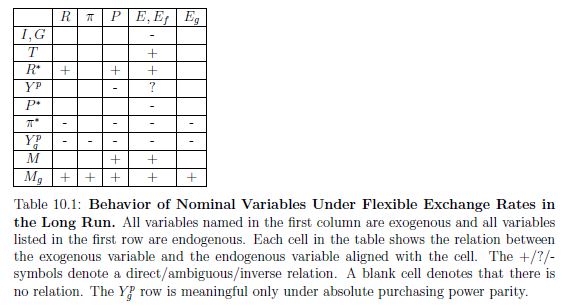
\includegraphics{images/nominal_long_flex.png}

}

\end{table}%

\subsection{Appreciation of the Nominal Exchange Rate}\label{sec-egflex}

By using Equation~\ref{eq-mg}, Equation~\ref{eq-eglr} can be rewritten
as \begin{equation}\phantomsection\label{eq-egflex}{
E_g=M_g-Y^p_g-\pi^*.
}\end{equation}

As all three variables on the right-hand side of this equation are
exogenous, this equation tells us all that can be said about the rate of
appreciation of the foreign currency: \emph{\(E_g\) is inversely
affected by \(\pi^*\) and \(Y^p_g\), directly affected by \(M_g\), and
unaffected by all other exogenous variables}. These ceteris paribus
effects are shown in the \(E_g\)-column of
Table~\ref{tbl-nominal_long_flex}.

\subsection{The Nominal Interest Rate}\label{sec-R-LR-flex}

Using Equation~\ref{eq-mg}, Equation~\ref{eq-nomintlong} can be
rewritten as \begin{equation}\phantomsection\label{eq-R-LR-flex}{
R=R^*-\pi^*- Y^p_g+M_g.
}\end{equation}

Again, note that all variables on the right-hand side of this equation
are exogenous. It follows that \emph{\(R\), the nominal interest rate,
is directly affected by \(R^*\) and \(M_g\), inversely affected by
\(\pi^*\) and \(Y^p_g\), and unaffected by all other exogenous
variables}. These ceteris paribus effects are shown in the \(R\)-column
of Table~\ref{tbl-nominal_long_flex}.

\subsection{The Price Level}\label{sec-pflex}

Equation~\ref{eq-LMlong} and Equation~\ref{eq-R-LR-flex} can be combined
into: \begin{equation}\phantomsection\label{eq-pflex}{
P=\frac {M}{L(R^*-\pi^*- Y^p_g+M_g)\cdot Y^p}.
}\end{equation}

Note that the above equation expresses the long-run equilibrium price
level entirely in terms of exogenous variables. Therefore, the above
equation tells us all that can be said about the price level.

Recall from Section~\ref{sec-mdemanddet} that \(L\) is inversely related
to \(R=R^*-\pi^*- Y^p_g+M_g\). Therefore, an increase in either \(R^*\)
or \(M_g\) or both (or a decrease in either \(\pi^*\) or \(Y^p_g\) or
both) will raise \(R\), reduce \(L\), and, therefore, raise \(P\). It
follows that \emph{the price level, \(P\), is directly affected by
\(M\), \(R^*\) and \(M_g\), inversely affected by \(Y^p\), \(Y^p_g\),
and \(\pi^*\), and unaffected by all other exogenous variables}. These
ceteris paribus effects are shown in the \(P\)-column of
Table~\ref{tbl-nominal_long_flex}.

\subsection{The Nominal Exchange Rate}\label{sec-eflex}

Equation~\ref{eq-q}, which defines the real exchange rate, can be
rewritten as \begin{equation}\phantomsection\label{eq-eflex}{
E=\frac {q\cdot P}{P^*}.
}\end{equation}

Consider the exogenous variables \(I\), \(G\) and \(T\). A quick look at
the previous section shows that they do not affect \(P\). Therefore,
their effects on \(E\) would be identical to their effects on \(q\),
which are described in Section~\ref{sec-longq} and shown in the
\(q\)-column of Table~\ref{tbl-real_long}. \%Under absolute purchasing
power parity, however, \(q=1\) always, which implies \(E=P/P^*\).

The foreign price level, \(P^*\), affects neither \(q\)---see
Section~\ref{sec-longq} ---nor \(P\)---see Section~\ref{sec-pflex}. It
is then obvious from Equation~\ref{eq-eflex} that \(E\) is inversely
related to \(P^*\).

An increase in \(R^*\) or \(M\) or \(M_g\) or a decrease in \(\pi^*\) or
\(Y^p_g\) (or some combination of these changes) will increase \(P\), as
we just saw in Section~\ref{sec-pflex}; have no effect on \(q\),
according to Section~\ref{sec-longq}; and have no effect on \(P^*\),
which is exogenous anyway. Therefore, by Equation~\ref{eq-eflex}, \(E\)
will increase.

\% Section~\ref{sec-longq} makes it clear that \(Y^p_g\), \(M\), and
\(M_g\) do not affect \(q\). As \(P^*\) is exogenous,
Equation~\ref{eq-eflex} implies that \(Y^p_g\), \(M\), and \(M_g\) can
affect \(E\) only through their effects on \(P\). According to
Section~\ref{sec-pflex}, an increase in \(M\) or \(M_g\) or a decrease
in \(Y^p_g\) will lead to an increase in \(P\), which, by
Equation~\ref{eq-eflex}, will lead to an increase in \(E\).

Finally, an increase in \(Y^p\) leads to an increase in \(q\) and a
decrease in \(P\) and leaves \(P^*\), which is exogenous anyway,
unchanged. Therefore, by Equation~\ref{eq-eflex}, the effect of \(Y^p\)
on \(E\) is ambiguous.

To summarize, \emph{the nominal exchange rate, \(E\), is inversely
affected by \(I\), \(G\), \(P^*\), \(\pi^*\), and \(Y^p_g\); directly
affected by \(T\), \(R^*\), \(M\), and \(M_g\); ambiguously affected by
\(Y^p\); and unaffected by all other exogenous variables}. These ceteris
paribus effects are shown in the \(E\)-column of
Table~\ref{tbl-nominal_long_flex}.

\subsection{The Future Value of the Nominal Exchange
Rate}\label{sec-efflex}

Can we make any predictions about the future value of the nominal
exchange rate (\(E_f\))?

As we saw in Section~\ref{sec-notngrowth}, the rate of appreciation of
the nominal exchange rate is \(E_g\equiv (E_f-E)/E\), which implies
\(E_f=(1+E_g)\cdot E\).

Now, let us consider the long-run behavior of \(E_g\) and \(E\), as
discussed in Section~\ref{sec-egflex} and Section~\ref{sec-eflex} and
summarized in the \(E\) and \(E_g\) columns of
Table~\ref{tbl-nominal_long_flex}. Note that there is no exogenous
variable whose effect on \(E_g\) contradicts its effect on \(E\).
Therefore, for every exogenous variable, its effect on \(E\) will be the
same as its effect on \(E_f=(1+E_g)\cdot E\). This is why the \(E\) and
\(E_f\) columns of Table~\ref{tbl-nominal_long_flex} are the same.

To summarize, \emph{the future value of the nominal exchange rate,
\(E_f\), is inversely affected by \(I\), \(G\), \(P^*\), \(\pi^*\), and
\(Y^p_g\); directly affected by \(T\), \(R^*\), \(M\), and \(M_g\);
ambiguously affected by \(Y^p\); and unaffected by all other exogenous
variables}.

This completes my discussion of the long-run behavior of nominal
variables in an economy that has a system of flexible exchange rates.
The results are summarized in Table~\ref{tbl-nominal_long_flex}.

\section{A Fixed Exchange Rate System}\label{sec-fix}

I will now try to describe the long-run behavior of the nominal
variables in an economy that has a system of fixed exchange rates.

Recall from Section~\ref{sec-fixexrates} that in a fixed exchange rate
system the nominal value of the domestic currency, \(E\) is exogenous
(because, after all, it is fixed!) and the quantity of money, \(M\), is
endogenous. It follows that \(M_g\), the growth rate of he quantity of
money, is endogenous as well.

\begin{table}

\caption{\label{tbl-nominal_long_fix}\textbf{Behavior of Nominal
Variables Under Fixed Exchange Rates in the Long Run.} All variables
named in the first column are exogenous and all variables listed in the
first row are endogenous. Each cell in the table shows the relation
between the exogenous variable and the endogenous variable aligned with
the cell. The +/?/- symbols denote a direct/ambiguous/inverse relation.
A blank cell denotes that there is no relation. The \(Y^p_g\) row is
meaningful only under absolute purchasing power parity.}

\centering{

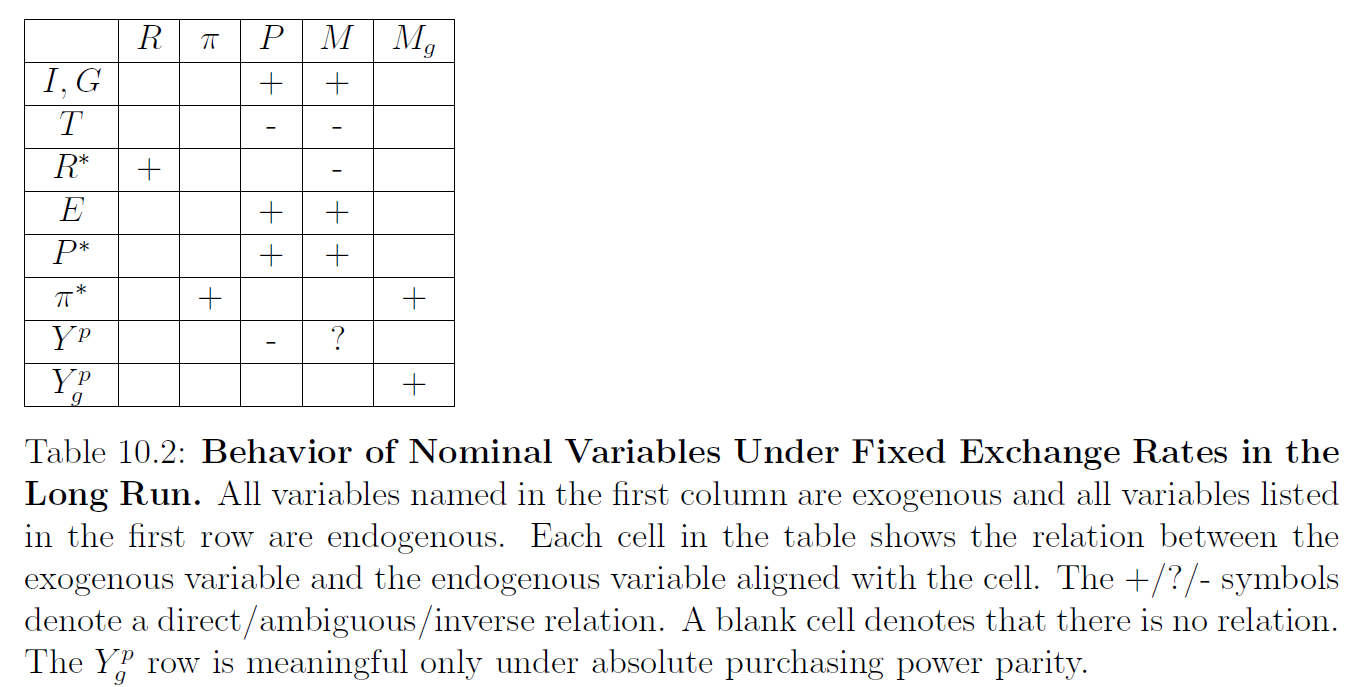
\includegraphics{images/nominal_long_fix.png}

}

\end{table}%

\subsection{Inflation}\label{sec-pifix}

As the value of \(E\) is exogenous and fixed, it follows that
\begin{equation}\phantomsection\label{eq-egfix}{
E_f=E\qquad\Longleftrightarrow\qquad E_g=0.
}\end{equation}

Equation~\ref{eq-eglr}, which is derived from the long-run assumption of
relative purchasing power parity, can then be rewritten as
\begin{equation}\phantomsection\label{eq-pifix}{
\pi=\pi^*.
}\end{equation}

That is, \emph{the domestic rate of inflation, \(\pi\), is equal to the
foreign rate of inflation, \(\pi^*\), and unaffected by all other
exogenous variables}. This is shown in the \(\pi\)-column of
Table~\ref{tbl-nominal_long_fix}.

\subsection{The Nominal Interest Rate}\label{sec-R-LR-fix}

Equation~\ref{eq-nomintlong} and Equation~\ref{eq-pifix} together imply
\begin{equation}\phantomsection\label{eq-R-LR-fix}{
R=R^*.
}\end{equation}

That is, \emph{the domestic nominal interest rate, \(R\), is equal to
the foreign nominal interest rate, \(R^*\), and is unaffected by all
other exogenous variables}. This is shown in the \(R\)-column of
Table~\ref{tbl-nominal_long_fix}.

Equation~\ref{eq-pifix} and Equation~\ref{eq-R-LR-fix} show how strongly
a country gets tied up with the country whose currency its own currency
is fixed to. If China fixes the value of its currency, the yuan, to,
say, 25 American cents, one yuan would essentially become equivalent to
a quarter dollar and the difference between people who carry yuans in
their wallets and those who carry dollars would be the same as the
difference between those who carry 25 cent coins in their wallets and
those who carry one dollar bills. In other words, when the yuan is fixed
to the dollar, there is no genuine difference any more between the two
currencies, which is why the inflation rates and interest rates in
America and China would become equal, just as they are equal in New York
and Texas and California.

\subsection{The Price Level}\label{sec-pfix}

Equation~\ref{eq-q}, which defines the real exchange rate, can be
rewritten as \begin{equation}\phantomsection\label{eq-pfix}{
P=\frac {E\cdot P^*}{q}.
}\end{equation}

As both \(E\) and \(P^*\) are exogenous, it follows that the exogenous
variables \(G\), \(I\), \(T\), and \(Y^p\) will affect \(P\) in a way
that is precisely the opposite of how Section~\ref{sec-longq} says they
affect \(q\).

Recall from Section~\ref{sec-longq} that \(E\), \(R^*\), \(\pi^*\) and
\(P^*\), being nominal variables, do not affect \(q\), the \emph{real}
exchange rate. Therefore, Equation~\ref{eq-pfix} implies that \(P\) is
directly affected by \(P^*\) and \(E\) and unaffected by \(R^*\) and
\(\pi^*\).

To summarize, \emph{\(P\) is directly affected by \(G\), \(I\), \(P^*\),
and \(E\), inversely affected by \(T\) and \(Y^p\) , and unaffected by
all other exogenous variables}. These ceteris paribus effects are shown
in the \(P\)-column of Table~\ref{tbl-nominal_long_fix}.

\subsection{The Quantity of Money}\label{sec-mfix}

Equation~\ref{eq-LMlong} and Equation~\ref{eq-R-LR-fix} together imply:
\begin{equation}\phantomsection\label{eq-mfix}{
M=L(R^*)\cdot P\cdot Y^p.
}\end{equation}

Therefore, for all exogenous variables other than \(R^*\) and \(Y^p\),
their effects on \(M\) are the same as what Section~\ref{sec-pfix} says
are their effects on \(P\).

According to Section~\ref{sec-mdemanddet}, \(L\) decreases when
\(R(=R^*)\) increases. Moreover, we saw in Section~\ref{sec-pfix} that
an increase in \(R^*\) has no effect on \(P\). Equation~\ref{eq-mfix}
then implies that \(M\) must decrease when \(R^*\) increases.

We also saw in Section~\ref{sec-pfix} that an increase in \(Y^p\)
decreases \(P\). Therefore, it folows from Equation~\ref{eq-mfix} that
the effect of an increase in \(Y^p\) on \(M\) is ambiguous.

To summarize, \emph{\(M\) is directly affected by \(G\), \(I\), \(P^*\),
and \(E\); inversely affected by \(T\) and \(R^*\); ambiguously affected
by \(Y^p\); and unaffected by all other exogenous variables}. These
ceteris paribus effects are shown in the \(M\)-column of
Table~\ref{tbl-nominal_long_fix}.

\subsection{Growth Rate of the Quantity of Money}\label{sec-mgfix}

Equations Equation~\ref{eq-mg} and Equation~\ref{eq-pifix} together
imply: \begin{equation}\phantomsection\label{eq-mgfix}{
M_g=\pi^*+ Y^p_g.
}\end{equation}

As both \(\pi^*\) and \(Y^p_g\) are exogenous, it follows that
\emph{\(M_g\) is directly affected by \(\pi^*\) and \(Y^p_g\), and
unaffected by all other exogenous variables}.

This completes my discussion of the long-run behavior of nominal
variables in an economy that has a system of fixed exchange rates. The
results are summarized in Table~\ref{tbl-nominal_long_fix}.

\subsection{The Sustainability of a Fixed Exchange Rate
System}\label{sec-fixexsys-sustainability}

\index{exchange rate!fixed!sustainability}\index{central banks!control of exchange rates}

Before we end this discussion of long-run international macroeconomics
under fixed exchange rates, let us go back to
Section~\ref{sec-fixexrates-money} of Chapter~\ref{sec-exchsys} and
remind ourselves of how a fixed exchange rate system works.

The domestic central bank announces that it is willing to buy/sell
currencies at the rate of \(\bar{E}\) units of the domestic currency per
unit of the foreign currency. Soon after this policy is announced, the
market equilibrium value of the foreign currency becomes equal to the
domestic central bank's target rate---\(E=\bar{E}\)---and the domestic
central bank achieves its wish to control \(E\).

Unfortunately, as was pointed out in Section~\ref{sec-fixexrates-money},
the domestic central bank will no longer be able to exert control over
the domestic money supply (\(M\)), which then becomes an endogenous
variable. When people show up at the domestic central bank's door with
bundles of foreign currency and ask for \(\bar{E}\) units of the
domestic currency for every unit of foreign currency, the domestic
central bank will have to print new currency and hand it over to the
public. There will, therefore, be a simultaneous \emph{increase} in the
domestic money supply (\(M\)) and the domestic central bank's reserves
of the foreign currency, which I will denote \(F\).

On the other hand, when people approach the domestic central bank,
offering \(\bar{E}\) units of the domestic currency and seeking one unit
of the foreign currency in exchange, the domestic central bank must
reach into its foreign currency reserves and hand over the promised
amount to the public. Therefore, in this case, there will be a
simultaneous \emph{decrease} in both \(M\) and \(F\).

In short, in a fixed exchange rate system, domestic money supply (\(M\))
and domestic reserves of foreign currency (\(F\)) must move together in
lockstep.

This brings us to Section~\ref{sec-mfix} above. There we saw that the
long-run equilibrium value of \(M\) could decrease for a number of
reasons---for example, decreases in domestic investment (\(I\)) and/or
foreign prices (\(P^*\)). Now, a money supply decrease of magnitude
\(\Delta M\) would have to be accompanied by a decrease in foreign
currency reserves of magnitude \(\Delta F=\Delta M/\bar{E}\). This is
because the people will show up at the domestic central bank's door,
hand over \(\Delta M\) units of the domestic currency, and ask for
\(\Delta F\) units of the foreign currency in return.

But what if the central bank just does not have \(\Delta F\) units of
the foreign currency?

In that case, unless a benevolent foreign government or an international
financial institution such as the International Monetary Fund steps in
with a loan, the domestic central bank will be forced to take back its
promise to exchange \(\bar{E}\) units of the domestic currency for each
unit of foreign currency. It will have to say, ``Sorry, but the deal is
off'' and put an end to the fixed exchange rate system. The economy
would thereafter operate under flexible exchange rates.

Aside from the prospect of being rescued by a foreign-currency loan from
a foreign government or the IMF, our discussion in
Section~\ref{sec-mfix} shows another way out: the government can come to
the central bank's rescue and either raise government spending
(\(G\uparrow\)) or cut taxes (\(T\downarrow\)). As can be checked from
the \(M\)-column of Table~\ref{tbl-nominal_long_fix}, these policy
measures will exert upward pressure on \(M\) and, thereby, reverse the
initial decline in \(M\) that was caused by decreases in \(I\) and/or
\(P^*\). This would remove the threat to the fixed exchange rate system.

However, such expansionary fiscal policies---big increases in government
spending and/or big cuts in taxes---will almost surely require deficit
financing or, simply, borrowing by the government. And at a time of
grave crisis, when the country's central bank is about to renege on its
promise, the credibility of the country's government may be low and
people may not be willing to lend it money. In that case, this country's
fixed exchange rate system would be hard to rescue.

We can learn more about the robustness of a country's fixed exchange
rate system by looking at the long-run equilibrium \emph{growth rate of
its money supply}. This is given in Equation~\ref{eq-mgfix}:
\(M_g=\pi^*+ Y^p_g\). Although this will most likely be positive, a
negative value cannot be ruled out. That would mean continuous and
simultaneous decreases in both \(M\) and \(F\). And, again, if the
domestic central bank does not have enough foreign currency reserves to
begin with, \(F\) could quickly evaporate, in which case the central
bank would have to put an end to its fixed exchange rate system.

To summarize the discussion so far, the sustainability of a fixed
exchange rate system depends crucially on whether the domestic central
bank has a big enough stash of foreign currency. One way for the
domestic central bank to ensure this is to adopt what is called a
\textbf{currency board} system.\index{currency board} In this case the
domestic central bank adopts a fixed exchange rate system only when its
foreign currency reserves (\(F\)) are at least \(1/\bar{E}\) times the
currency held by the public.

To see why this will ensure that the central bank will never run out of
foreign currency, let's try a numerical example. Suppose the amount of
domestic currency currenctly held by the public is \$10 trillion.
Suppose the domestic central bank announces that it is willing to
exchange currencies at the rate of \$2.00 for \EUR{1.00}: this sets
\(\bar{E}=2\). If domestic reserves of foreign currency are currently
\((1/2)\times 10 =\) \EUR{5.00} trillon, then even if all \$10 trillion
currently held by the public are brought to the central bank by people
clamoring for euros in return, the central bank would still have enough
euros to keep its promise. It will not run out of foreign currency
reserves.

I will continue my discussion of the sustainability of fixed exchange
rate systems and their susceptibility to speculative currency crises in
a later chapter.

\section{Conclusion: Flexible or Fixed?}\label{sec-flexorfix}

Now that we have looked at the long-run behavior of nominal economic
variables under both flexible and fixed exchange rate systems, which
system is better?

A lot comes down to the extent to which a country can neutralize the
effects on its economy of things that may be happening in another
country.

If it is very important for a country to be able to keep its inflation
rate stable and unaffected by economic shocks originating abroad, then a
flexible exchange rate system would be preferable.
Equation~\ref{eq-piflex} shows that \(\pi=M_g-Y^p_g\) under a flexible
system and Equation~\ref{eq-pifix} shows that \(\pi=\pi^*\) in a fixed
system. Under a fixed exchange rate system, a country's inflation rate
is joined at the hip to the foreign country's inflation.

On the other hand, under a fixed exchange rate system, the exchange rate
is, well, fixed, whereas under a flexible exchange rate system traders
engaged in international transactions may have to grapple with a lot of
uncertainty over the exchange rate.

In the end, it all comes down to the relative importance of inflation
stability versus exchange rate stability for a particular country.

\bookmarksetup{startatroot}

\chapter{Short-Run Predictions: Fixed Exchange
Rates}\label{sec-short-fixed}

In the last two chapters, we have seen how a country is affected in the
long run by permanent changes in exogenous variables. For example, we
saw in Chapter~\ref{sec-longreal} that a permanent cut in government
spending (\(G\downarrow\)) leads to an increase in a country's net
exports (\(NX\uparrow\)) in the long run. And in
Chapter~\ref{sec-longnom} we saw that in the long run a permanent
increase in the foreign inflation rate (\(\pi^*\)) will raise the
domestic inflation rate (\(\pi\)) under fixed exchange rates but not
under flexible exchange rates.\footnote{Take a quick peek at
  Table~\ref{tbl-real_long}, Table~\ref{tbl-nominal_long_flex}, and
  Table~\ref{tbl-nominal_long_fix} for a refresher on the predictions of
  long-run international macroeconomics.}

The questions that we wrestle with in this and the next two chapters are
not about the long run. Specifically, our questions will now follow this
general format: If there is an increase in {[}some exogenous
variable{]}, what will happen in the short run to {[}some endogenous
variable{]}? If a country is hit by a recession and lots of people begin
to lose their jobs, what could turn things around in a relatively short
amount of time? Would a temporary tax cut have the desired effect? The
relevance of such questions is obvious.

This chapter considers an economy that has a fixed exchange rate
system.\footnote{See Section~\ref{sec-fixexrates} for a discussion of
  the fixed exchange rate system.} The next two chapters will consider
flexible exchange rates. Although flexible exchange rate systems are far
more widespread than fixed exchange rate systems, I chose to discuss
fixed exchange rates first mainly because the analysis is somewhat
simpler.

\section{The short run needs a different
approach}\label{sec-short-run-approach}

But first, why do we need separate chapters for long-run analysis and
short-run analysis? Why can't we make do with the last two chapters? Why
wouldn't the long-run analysis of the last two chapters be applicable in
the short run as well?

\subsection{Recessions and Booms}\label{sec-recessions-booms}

To see why, recall from Section~\ref{sec-longana} that long-run analysis
\emph{assumes} full employment. That is, an economy's real gross
domestic product (\(Y\)) is assumed to be equal to its potential real
gross domestic product (\(Y^p\)). In other words, recessions and booms
are ruled out \emph{by assumption}. This short-cut is fine for long-run
analysis, but not for short-run analysis.

Sudden and sharp declines in \(Y\) do happen. Therefore, such recessions
need to be explained. A theory that assumes \(Y=Y^p\) can ``explain'' a
sharp decline in \(Y\) by arguing that there must have been a sharp
decline in \(Y^p\). But such an explanation is unpersuasive. After all,
as we saw in Section~\ref{sec-pgdp}, the factors that determine a
country's potential GDP---the quantity and quality of productive
resources, the level of technology, and the nature of the country's
institutions---typically do not go up and down like a yoyo. Therefore,
for short-run analysis, the only way to reconcile a stable \(Y^p\) with
a volatile \(Y\) is by rejecting the \(Y=Y^p\) assumption and admitting
that recessions (\(Y<Y^p\)) and booms (\(Y>Y^p\)) may happen.

\subsection{Price Rigidity}\label{sec-p-rigidity}

A related question is this: What might make \(Y\) less than \(Y^p\)? If
an economy is capable of producing \$14 trillion worth of goods and
services per year under normal circumstances, why would it not produce
that amount? Why would it produce less? Or more? The key reason is that
prices tend to be sticky (or `rigid' or `inflexible') in the short run.

In the long run, changes in the price level (\(P\)) tend to yank \(Y\)
towards \(Y^p\) whenever the two diverge. In recessions (\(Y<Y^p\)),
unemployment rises. The availability of many unemployed workers seeking
jobs tends to make labor cheaper. This induces businesses to hire
additional workers and boost production. To sell the additional output,
firms must reduce prices, and indeed they can afford to do so because
the wages they pay their workers have fallen. So, a recovery occurs and
\(Y\) again becomes equal to \(Y^p\) thanks to the flexibility of wages
and prices. This ability of the price level to respond flexibly to a
recession and restore full employment is what makes the \(Y=Y^p\)
assumption reasonable in long-run analysis.

Unfortunately, this smooth self-adjusting process tends not to work in
the short run. In the short run, wages may \emph{not} fall in a
recession---the presence of many unemployed job seekers
notwithstanding---because of contracts that were agreed upon among
businesses and workers or because of several other reasons. Wages are
\emph{sticky} in the short run. And, the stickiness of wages typically
means sticky prices as well. Moreover, prices may be sticky for reasons
unrelated to the stickiness of wages. And this price stickiness could
make it difficult for businesses to hire more workers during a recession
because the additional output produced by the newly hired workers will
not sell if prices cannot be reduced.

\subsection{Expectations}\label{sec-sr-expectations}

Another distinction between long-run analysis and short-run analysis has
to do with expectations. As we saw in Section~\ref{sec-shortana},
short-run analysis assumes that \(E_f^e\), which is what the value of
the foreign currency at a future date is currently expected to be, is
equal to \(E_{fLR}\), which is the long-run equilibrium value of
\(E_f\). Moreover, \(E_{fLR}\) is assumed to be \emph{exogenous}.
Long-run analysis, on the other hand, assumes perfect foresight:
\(E_f^e=E_f\). This is equivalent to the \(E_f^e=E_{fLR}\) assumption of
short-run analysis except that \(E_{fLR}\) is \emph{endogenous} in
long-run analysis.

The distinction is hard to explain, but let me try. For both long-run
analysis and short-run analysis we assume \(E_f^e=E_{fLR}\). That is, we
assume that people's expectations about \(E_f\) will coincide with its
actual long-run equilibrium value. In long-run analysis, as we saw in
Section~\ref{sec-efflex}, \(E_f\) is an endogenous and unknown
variable---like \(E\), \(R\), \(P\), \(\pi\), etc.---whose equilibrium
value is determined by the theory itself; that is why
Table~\ref{tbl-nominal_long_flex} has an entire column listing how the
various exogenous variables affect the long-run equilibrium value of
\(E_f\). Short-run analysis, on the other hand, is unable to determine
the value of \(E_{fLR}\). It treats \(E_{fLR}\) as a mysterious,
exogenous variable that dances to its own tune. It has to seek the
assistance of long-run analysis to understand what makes \(E_{fLR}\)
increase or decrease.

The distinction between the long-run and short-run assumptions about
expectations is key to understanding why the short-run effects of a
\emph{temporary} change in an exogenous variable are different from the
short-run effects of a \emph{permanent} change in that same exogenous
variable. A temporary change in an exogenous variable---for example, a
temporary cut in taxes (\(T\downarrow\))---cannot be expected to affect
the future. Therefore, it makes sense to assume that people's
expectations about the future (\(E_f^e\)) will be unaffected. As a
result, the short-run analysis of a \emph{temporary} tax cut can proceed
on the assumption that \(E_f^e\) has not changed. The short-run analysis
of a \emph{permanent} tax cut is a more complex matter.
Table~\ref{tbl-nominal_long_flex}, which summarizes the long-run
analysis of a flexible exchange rate system, says that a permanent tax
cut will reduce \(E_{fLR}\). Knowing this, the people will rationally
revise \(E_f^e\) downward as soon as the permanent tax cut is announced.
Therefore, the short-run effect of a \emph{permanent} tax cut is the
\emph{combined effect} of a \emph{temporary tax cut}and a decrease in
\(E_f^e\).

We will discuss this issue further in the next two chapters.

\section{Short-Run Equilibrium in the Goods
Market}\label{sec-goodseqm-shortfix}

We are now ready to do what we did in Chapter~\ref{sec-longreal} and
Chapter~\ref{sec-longnom}, but under the short-run assumptions that both
\(P\) and \(E_f^e\) are exogenous. Unfortunately, short-run analysis is
not as straightforward as long-run analysis. The arguments will have to
be built up brick-by-brick and a full view of the theory will not be
visible for quite a while. You will have to be patient.

The foundation of the theory will once again consist of the equations
for equilibrium in the goods, money, and foreign currency markets that
we saw in Chapter~\ref{sec-basicequations}. So, it might be a good idea
for you to review Equation~\ref{eq-IS}, Equation~\ref{eq-LM}, and
Equation~\ref{eq-UIP-alt}.

\subsection{The Aggregate Expenditure Curve}\label{sec-aecurve}

\index{aggregate expenditure curve}

Recall from Section~\ref{sec-goodseqm} that equilibrium in the goods
market requires that the demand for domestically produced goods be equal
to the output of such goods, as in Equation~\ref{eq-IS}. This crucial
equation is reproduced below, with Equation~\ref{eq-q} or
\(q=E\cdot P^*/P\) substituted for \(q\):
\begin{equation}\phantomsection\label{eq-IS-shortfix}{
\fbox{$\displaystyle Y=C(Y-T)+I+G+NX\left(\frac{E\cdot P^*}{P},Y-T\right).$}
}\end{equation}

Note that \(Y\) is the only endogenous variable in the above equation.
As we saw in Section~\ref{sec-exoendo} that \(T\), \(I\), \(G\), and
\(P^*\) are always exogenous in these lectures. Moreover, as we saw
above, \(P\) is exogenous in short-run analysis. And, finally, \(E\) is
exogenous because we are considering fixed exchange rates in this
chapter. That leaves \(Y\) as the only endogenous variable in
Equation~\ref{eq-IS-shortfix}. This implies that an analysis of this
equation will tell us all that can be said about the short-run behavior
of \(Y\) under fixed exchange rates.\footnote{See
  Theorem~\ref{thm-eqnno} in Section~\ref{sec-howmanyeq} for a quick
  reminder.}

The analysis of Equation~\ref{eq-IS-shortfix} will now proceed, not
algebraically but graphically. (Indeed, you will see that a lot of
short-run analysis is graphical.)

As was mentioned in the first paragraph of this section, the right-hand
side of Equation~\ref{eq-IS-shortfix} represents the total expenditure
on domestically produced goods. This is usually referred to as
\textbf{aggregate expenditure} or \(AE\).\index{aggregate expenditure}
The goods market equilibrium condition can then be stated simply as
\(Y=AE\). \(C\), \(I\), \(G\), and \(NX\) are called the *components of
aggregate expenditure.\footnote{See Section~\ref{sec-goodseqmdef} for
  more on aggregate expenditure and its components.}

We saw in Section~\ref{sec-consumption} that a country's consumption
spending (\(C\)) is represented by the consumption function
\(C=C(Y-T)\). We assume that \(C\) is directly related to income (\(Y\))
and inversely related to taxes (\(T\)).
Figure~\ref{fig-consumption_function} showed the consumption function
graphically as a rising consumption curve. Moreover,
Figure~\ref{fig-consumption_function} also shows that the consumption
curve shifts downward when taxes increase. The consumption curve of
Figure~\ref{fig-consumption_function} makes a return appearance in
figure Figure~\ref{fig-AE} in this chapter.

As we saw in Section~\ref{sec-investment} and Section~\ref{sec-gov},
business investment (\(I\)) and government spending (\(G\)) are assumed
to be exogenous constants; in particular, they do not go up or down when
\(Y\) increases or decreases. In figure Figure~\ref{fig-AE} they are
therefore represented by horizontal lines.

If we stack the \(C\), \(I\), and \(G\) curves one on top of the other,
we get the \(C+I+G\) curve in figure Figure~\ref{fig-AE}. \(C+I+G\) is
commonly referred to as \textbf{gross domestic purchases}, the total
purchases of domestic households, firms, and government.

We saw in Section~\ref{sec-summary-nxp} that a country's net exports are
given by \(NX=NX(q,Y-T)\) and that net exports are directly related to
the real exchange rate (\(q\)) and to \(T\), and inversely related to
\(Y\). Figure Figure~\ref{fig-net_exports_general} showed this
graphically. Its right panel, in particular, shows a net exports curve
that slopes downward as \(Y\) increases and shifts downward when either
\(q\) or \(T\) falls. This net exports curve makes a return appearance
in figure Figure~\ref{fig-AE} here.

If we stack the \(C\), \(I\), \(G\), and \(NX\) curves vertically, we
get the aggregate expenditure (\(AE=C+I+G+NX\)) curve in figure
Figure~\ref{fig-AE}. At any particular value of real GDP (\(Y\)), the
height of the \(AE\) curve shows the total demand for domestically
produced goods.

\subsection{\texorpdfstring{Slope of the \texorpdfstring{$AE$}{AE}
Curve}{Slope of the  Curve}}\label{sec-aeslope}

Note that the \(AE\) curve is upward sloping. Would it be a mistake to
draw it as a downward-sloping curve instead? Recall that the \(I\) and
\(G\) curves are horizontal, the \(C\) curve is upward sloping, and the
\(NX\) curve is downward sloping. When these curves are stacked
vertically to construct the \(AE\) curve, couldn't the result be a
downward-sloping curve?

Well, no. A quick look at Section~\ref{sec-imports} will settle the
issue. When income (\(Y\)) increases, so does consumption (\(C\)). Only
a part of that additional consumption is imported. That is, imports
increase, but by less than the magnitude of the increase in consumption.
As exports are unaffected by \(Y\), net exports (\(NX\)) will decrease,
but again by less than the magnitude of the increase in \(C\).
Therefore, \(AE=C+I+G+NX\) will increase when \(Y\) increases, which
means that the \(AE\) curve in figure Figure~\ref{fig-AE} has been quite
properly shown to be upward sloping.

Note that \(NX\) can be positive or zero or negative. At \(Y=Y_A\) in
figure Figure~\ref{fig-AE}, \(NX=0\), which is why the gross domestic
purchases (\(C+I+G\)) curve and the aggregate expenditure
(\(AE=C+I+G+NX\)) curve have the same height (that is, they intersect)
at \(Y=Y_A\). At lower incomes (\(Y<Y_A\)), \(NX>0\) and, therefore,
\(AE\) exceeds \(C+I+G\). At higher incomes (\(Y>Y_A\)), \(NX<0\) and,
therefore, \(AE\) is less than \(C+I+G\).

\subsection{\texorpdfstring{The 45\texorpdfstring{$^{\circ}$}{-Degree}
Line}{The 45 Line}}\label{sec-45degline}

Figure Figure~\ref{fig-AE} also includes a 45\(^{\circ}\) line through
the origin. To see the utility of this seemingly useless line, note that
at any value of \(Y\), the height of the 45\(^{\circ}\) line is equal to
the value of \(Y\). For instance, at \(Y=Y_A\), the height up to point
\(B\) on the 45\(^{\circ}\) line is \emph{equal} to \(Y_A\), whereas the
height up to point \(A\) on the \(AE\) curve \emph{exceeds} \(Y_A\). As
the height of the \(AE\) curve denotes the magnitude of \(AE=C+I+G+NX\),
it follows that at \(Y=Y_A\), \(Y<AE\), which violates
Equation~\ref{eq-IS-shortfix}, the equilibrium condition for the goods
market. So, simply by noting that the \(AE\) curve is higher than the
45\(^{\circ}\) line at \(Y=Y_A\), one can conclude that it would be
unwise to predict that \(Y=Y_A\) in short-run equilibrium.

\begin{figure}

\centering{

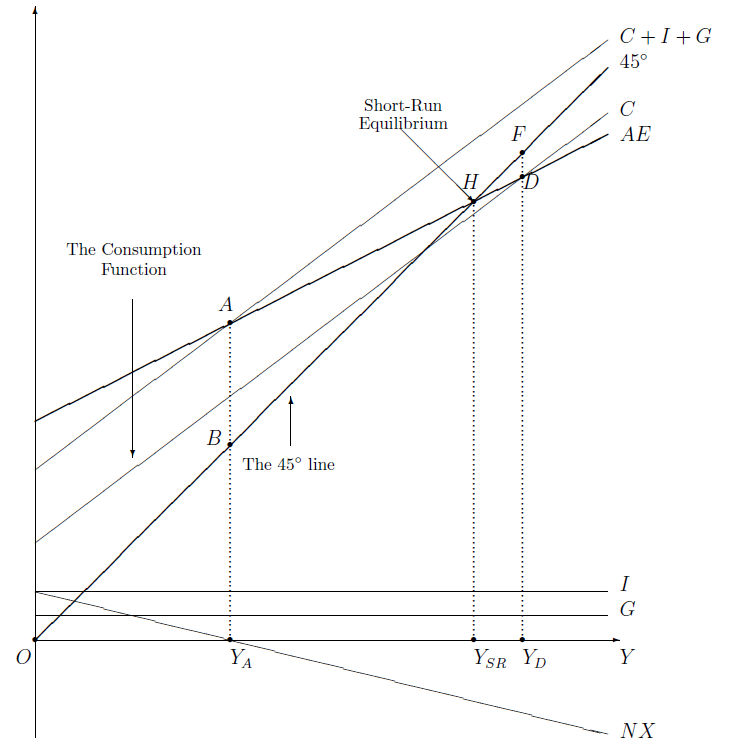
\includegraphics{images/keynesian_cross.png}

}

\caption{\label{fig-AE}Here we see how the short-run equilibrium value
of \(Y\) can be graphically determined if the aggregate expenditure
curve (\(AE\)) is known. The \(AE\) curve is constructed by the vertical
summation of the consumption (\(C\)), investment (\(I\)), government
spending (\(G\)), and net exports (\(NX\)) curves. The goods market is
in equilibrium when \(Y=AE\)---that is, when the \(AE\) curve intersects
the 45\(^{\circ}\) line.}

\end{figure}%

\subsection{The Keynesian Cross}\label{sec-keynes-cross}

Now that we have ruled out \(Y_A\), could the short-run equilibrium
value of \(Y\) be \(Y_D\) instead? At \(Y=Y_D\), a comparison of points
\(D\) and \(F\) shows that the height of the \(AE\) curve is \emph{less}
than the height of the 45\(^{\circ}\) line. Therefore, \(Y>AE\) at
\(Y=Y_D\). So, \(Y_D\) can't be the short-run equilibrium GDP either.

So far, we have tried twice to spot the equilibrium value of \(Y\) and
have failed miserably. At \(Y_A\), the \(AE\) curve was higher than the
45\(^{\circ}\) line. At \(Y_D\), the \(AE\) curve was lower than the
45\(^{\circ}\) line. So, it makes sense to try point \(H\) where the two
curves cross. At \(Y=Y_{SR}\), the heights of the two curves are same,
implying \(Y=AE\). Therefore, the short-run equilibrium value of real
GDP must be \(Y=Y_{SR}\).

That's it, we've finally got it! We have established that \emph{if a
country's \(AE\) curve is known, its short-run equilibrium GDP is the
value of \(Y\) at which the \(AE\) curve crosses the 45\(^{\circ}\)
line}.

As you will soon see, this graphical trick will be very useful in
predicting how GDP is affected by changes in various exogenous
variables.

\begin{figure}

\centering{

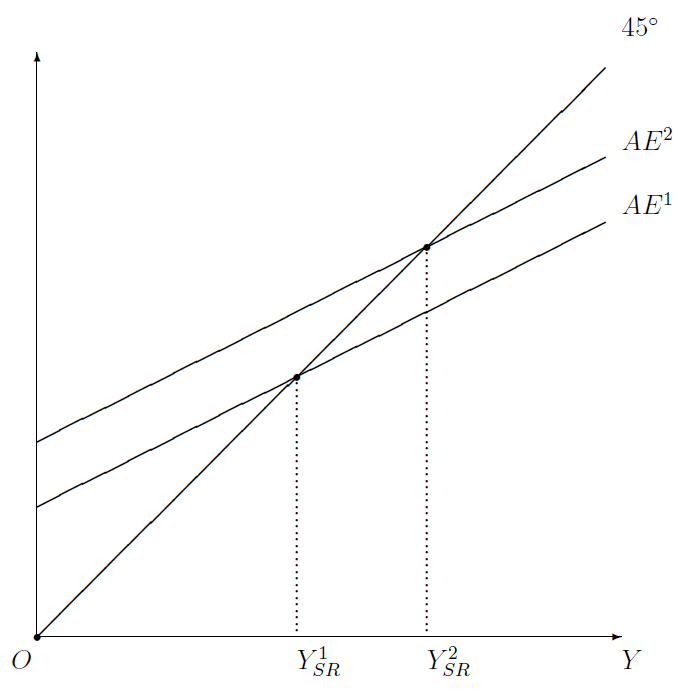
\includegraphics{images/keynesian_cross_with_shift.png}

}

\caption{\label{fig-AE-shifts}An upward shift of the aggregate
expenditure curve leads to an increase in GDP in the short run. Such an
upward shift of the \(AE\) curve could be caused by an increase in \(G\)
or \(I\) or \(E\) or \(P^*\), or by a decrease in \(T\) or \(P\), or by
some combination of these changes. Therefore, in the short run and under
fixed exchange rates, \(Y\) is directly affected by \(G\), \(I\), \(E\),
and \(P^*\); inversely affected by \(T\) and \(P\), and unaffected by
all other exogenous variables.}

\end{figure}%

\subsection{\texorpdfstring{Gross Domestic Product: How the \(AE\) curve
can
shift}{Gross Domestic Product: How the AE curve can shift}}\label{sec-AE-shifts}

\index{aggregate expenditure curve}

In figure Figure~\ref{fig-AE-shifts}, there are two aggregate
expenditure curves, \(AE^1\) and \(AE^2\), as well as the 45\(^{\circ}\)
line that first appeared in figure Figure~\ref{fig-AE}. Given that the
short-run equilibrium level of income is that at which the \(AE\) curve
crosses the 45\(^{\circ}\) line, it follows that equilibrium income must
be \(Y_{SR}^1\) when aggregate expenditure is \(AE^1\) and \(Y_{SR}^2\)
when aggregate expenditure is \(AE^2\). In other words, \emph{the higher
the \(AE\) curve, the higher the short-run equilibrium income}.

Therefore, if we knew what makes the aggregate expenditure curve rise,
we would know what makes income increase.

Luckily, it is straightforward to figure out what makes the \(AE\) curve
rise (or fall). Recall from Section~\ref{sec-aecurve} that the \(AE\)
curve is the vertical sum of the \(C\), \(I\), \(G\), and \(NX\) curves.
Therefore, anything that causes any of these curves to shift upwards
will also shift the \(AE\) curve upwards.

We saw in Section~\ref{sec-consumption} and figure
Figure~\ref{fig-consumption_function} that a decrease in taxes
(\(T\downarrow\)) shifts the \(C\) curve up. An increase in households'
wealth---possibly fueled by a rise in share prices or home
prices---would have the same effect, as would a general surge in
optimism. Therefore, any combination of these factors would shift the
\(AE\) curve upwards as well.

A surge in optimism among entrepreneurs will cause business investment
to increase. This would raise the \(I\) curve and, therefore, the \(AE\)
curve.

A shift in government policy---brought about, say, by the election of a
new president---could boost government spending. This would raise the
\(G\) curve and, consequently, the \(AE\) curve.

As was pointed out in Figure~\ref{fig-net_exports_general}, an increase
in either taxes (\(T\uparrow\)) or the real exchange rate
(\(q\uparrow\)) shifts the net exports curve upwards. Of course, we know
from Equation~\ref{eq-q} that \(q=E\cdot P^*/P\). Therefore, we can say
that the \(NX\) and \(AE\) curves would shift upwards if \(E\) increases
or \(P^*\) increases or \(P\) decreases. In all these cases, the \(NX\)
curve rises and, therefore, so does the \(AE\) curve.\footnote{Increases
  in foreign incomes or in the rate of tariffs on imported goods would
  have similar positive effects on the \(AE\) curve, but these variables
  are not formally considered here.}

There is a slight problem, however, with the effect of taxes. A tax cut
(\(T\downarrow\)) \emph{raises} the \(C\) curve and \emph{lowers} the
\(NX\) curve, simultaneously. What's the overall effect on these
conflicting effects on the \(AE\) curve? As this issue was addressed
indirectly in Section~\ref{sec-aeslope}, I don't want to rehash the
argument here. Long story short, when taxes fall, consumption increases
and so do imports, but by a smaller amount. As a result, the \(C\) curve
shifts up and the \(NX=\hbox{exports}-\hbox{imports}\) shifts down, but
the increase in \(C\) exceeds the decrease in \(NX\). Therefore, the
\(AE\) curve shifts \emph{up}.

To summarize, \emph{in an economy that has a fixed exchange rate system,
the aggregate expenditure curve shifts upwards---and, therefore,
short-run equilibrium income (\(Y\)) rises---if there is a ceteris
paribus decrease in \(T\) or \(P\), or there is a ceteris paribus
increase in \(I\) or \(G\) or \(E\) or \(P^*\), or there is some
combination of those changes. Changes in other exogenous variables will
have no effect}. This is shown in the \(Y\)-column of
Table~\ref{tbl-short_fixed}.

\subsection{Consumption}\label{sec-c-shortfix}

What can we say about the short-run behavior of consumption spending
under fixed exchange rates? For example, how will \(C\) react if \(T\)
increases? Recall that \(C=C(Y-T)\). We have just seen that \(Y\)
decreases when \(T\) increases. This decrease in \(Y\) coupled with the
increase in \(T\) implies that disposable income (\(Y-T\)) will
decrease. Therefore, \(C\) must decrease.

Changes in the other exogenous variables---\(I\), \(G\), \(P^*\), \(E\),
and \(P\)---cannot affect \(T\), which is exogenous. Therefore, their
effects on \(C=C(Y-T)\) will be the same as their effects on \(Y\). That
is why the \(C\) and \(Y\) columns of Table~\ref{tbl-short_fixed} are
the same for these five exogenous variables.\footnote{For example, when
  \(G\) increases, \(Y\) increases and \(T\) is unaffected. Therefore,
  \(Y-T\) increases. Therefore, \(C\) increases as well. The effect of
  \(G\) on \(Y\) is the same as the effect of \(G\) on \(C\).}

To summarize, \emph{in an economy that has a fixed exchange rate system,
in the short-run equilibrium, \(C\) is directly affected by \(I\),
\(G\), \(P^*\), and \(E\), inversely affected by \(T\) and \(P\), and
unaffected by all other exogenous variables}. These ceteris paribus
effects are shown in the \(C\)-column of Table~\ref{tbl-short_fixed}.

\subsection{Net Exports}\label{sec-nx-shortfix}

To analyze the behavior of net exports, I will make use of the
behavioral expression \(NX=NX(E\cdot P^*/P,Y-T)\) and the goods market
equilibrium condition, which yields \(NX=Y-C(Y-T)-I-G\).\footnote{These
  two ways of looking at \(NX\) were also jointly deployed in the
  long-run analysis of the real exchange rate (\(q\)) in
  Section~\ref{sec-longq}.}

First, consider an increase in \(I\) or an increase in \(G\) or a
decrease in \(T\). The \(Y\)-column of Table~\ref{tbl-short_fixed}
assures us that \(Y\) will increase. Therefore, disposable income
(\(Y-T\)) will increase too. Moreover, \(E\cdot P^*/P\) will be
unaffected as \(E\), \(P^*\), and \(P\) are all exogenous and,
therefore, cannot be affected by changes in other exogenous variables.
Therefore, \(NX=NX(E\cdot P^*/P,Y-T)\) must decrease, as net exports
fall when rising disposable income leads to surging imports---see
Section~\ref{sec-netexports}.

Second, check from Section~\ref{sec-AE-shifts} of from the \(Y\)-column
of Table~\ref{tbl-short_fixed} that an increase in \(R^*\) has no effect
on \(Y\). Moreover, it cannot affect \(E\), \(P\), \(P^*\), and \(T\).
Therefore, it cannot have any effect on \(NX=NX(E\cdot P^*/P,Y-T)\).

Finally, consider an increase in \(E\) or an increase in \(P^*\) or a
decrease in \(P\). The real exchange rate (\(q\equiv E\cdot P^*/P\))
increases. As we saw in Section~\ref{sec-AE-shifts} and as the
\(Y\)-column of Table~\ref{tbl-short_fixed} reminds us, an increase in
the relative price of foreign goods (that is, \(q\uparrow\)) will raise
the aggregate expenditure curve and cause \(Y\) to increase. The
simultaneous increase of \(q\) and \(Y-T\) will have \emph{conflicting}
effects on \(NX=NX(E\cdot P^*/P,Y-T)\): the rise in \(q\) increases
\(NX\) and the rise in \(Y-T\) decreases it.

To get away from this confusing ambiguity, let us look at
\(NX=Y-C(Y-T)-I-G\) instead. Recall from Section~\ref{sec-mpc} that when
\(Y\) increases, \(C\) increases but by a smaller amount. Therefore,
\(Y-C\) increases. As \(E\), \(P^*\), and \(P\) are exogenous, they have
no effect on \(I\) and \(G\), which are exogenous too. Therefore, we
conclude that if there is an increase in \(E\) or an increase in \(P^*\)
or a decrease in \(P\), \(NX=Y-C(Y-T)-I-G\) must increase.

To summarize, \emph{in an economy that has a fixed exchange rate system,
in the short-run equilibrium, a country's net exports (\(NX\)) is
directly affected by \(T\), \(P^*\), and \(E\), inversely affected by
\(I\), \(G\), and \(P\), and unaffected by all other exogenous
variables}. These ceteris paribus effects are shown in the \(NX\)-column
of Table~\ref{tbl-short_fixed}.

\subsubsection{Tariffs}\label{sec-tariffs-shortfix}

The effect of the nominal price of foreign goods (\(P^*\)) on net
exports can help us understand the effect of protectionist measures such
as \textbf{tariffs} \index{tariffs}, even though tariffs have not been
formally included in our equations. When tariffs are imposed on imported
goods, the effect is the same as that of an increase in \(P^*\), which,
as can be checked from the \(P^*\) row of Table~\ref{tbl-short_fixed},
leads to increases in both \(Y\) and \(NX\). Therefore, at least in the
short run and under fixed exchange rates, a tariff may not be a bad idea
for an economy that is suffering from either a recession or a huge trade
deficit.

However, the theory being discussed here is simple and needs a ``don't
try this at home'' warning. It assumes that a country can embrace
protectionist policies such as tariffs without provoking retaliation. In
the real world, a country that imposes tariffs will very quickly find
its trade partners implementing retaliatory tariffs.

\begin{table}

\caption{\label{tbl-short_fixed}\textbf{Macroeconomic Behavior under
Fixed Exchange Rates in the Short Run}. All variables named in the first
column are exogenous and all variables listed in the first row are
endogenous. Each cell in the table shows the relation between the
exogenous variable and the endogenous variable aligned with the cell.
The +/?/- symbols denote a direct/ambiguous/inverse relation. A blank
cell denotes that there is no relation.}

\centering{

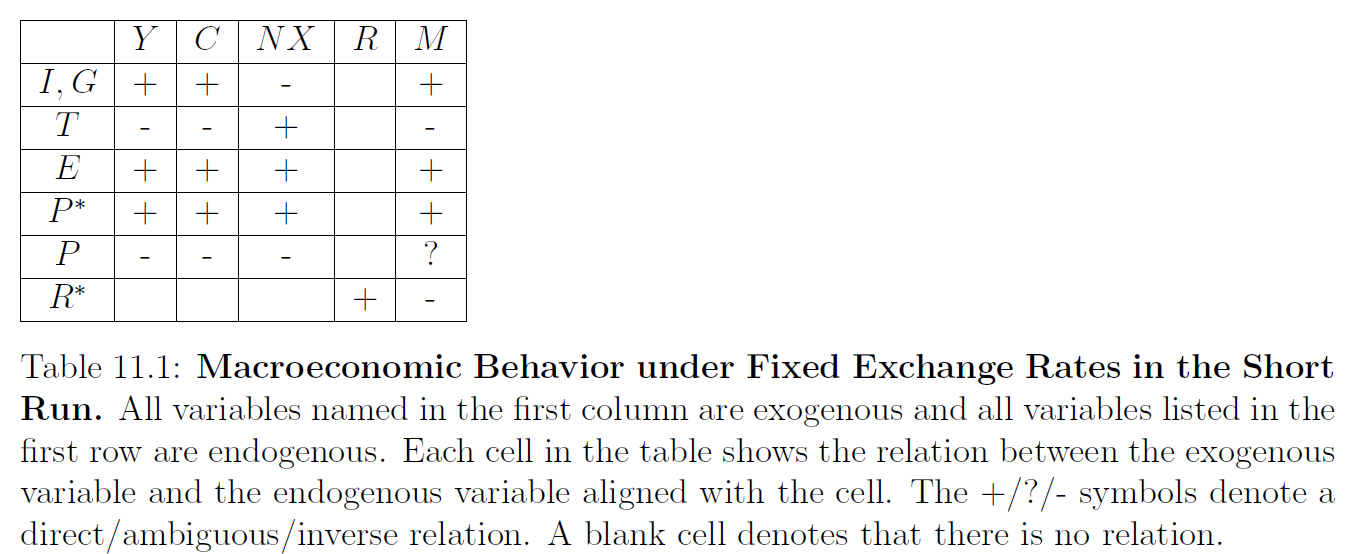
\includegraphics{images/short_fixed.png}

}

\end{table}%

\section{The Interest Rate: Short-Run Equilibrium in the Foreign
Currency Markets}\label{sec-asseteqm-shortfix}

Recall from Section~\ref{sec-summary-UIP} that equilibrium in the
foreign exchange market is represented by the uncovered interest parity
equation, Equation~\ref{eq-UIP-alt}, which is reproduced below: \[
R=R^*+\frac{E^e_f}{E}-1.
\]

Now, keep in mind that we are considering a fixed exchange rate regime
in this chapter. Assuming that the central bank's promise to keep the
exchange rate fixed is credible, people would expect the future value of
the exchange rate to be equal to its current value. That is, we have
\(E^e_f=E\), which, when inserted into the equation above, implies
\begin{equation}\phantomsection\label{eq-UIP-shortfix}{
\fbox{$\displaystyle R=R^*.$}
}\end{equation}

This says all that can be said about the nominal interest rate: \emph{in
the short-run equilibrium of an economy that has a fixed exchange rate
system, the domestic nominal interest rate is equal to the foreign
nominal interest rate. No other exogenous variable has any effect}. This
is shown in the \(R\)-column of Table~\ref{tbl-short_fixed}.

If, at this point, you are trying to make sense of a nagging feeling of
\emph{deja vu}, let me reassure you. The analysis of the nominal
interest rate under fixed exchange rates is exactly the same for both
the long run and the short run. See Section~\ref{sec-R-LR-fix} and
compare it to this section.

\section{The Quantity of Money: Short-Run Equilibrium in the Money
Market}\label{sec-moneyeqm-shortfix}

Recall from Section~\ref{sec-summary-moneyeqm} that equilibrium in the
money market requires the equality of money demand and money supply,
which is represented by Equation~\ref{eq-LM}. With the necessary
substitution of \(R=R^*\) from Equation~\ref{eq-UIP-shortfix} above, we
get \begin{equation}\phantomsection\label{eq-LM-shortfix}{
\fbox{$\displaystyle M=L(R^*)\cdot P\cdot Y.$}
}\end{equation}

Recall from Section~\ref{sec-fixexrates-money} that, in a fixed exchange
rate system, a country's money supply is an endogenous variable.
Equation~\ref{eq-LM-shortfix}, therefore, has two exogenous variables,
\(R^*\) and \(P\), and two endogenous variables, \(Y\) and \(M\).
However, as we already know how various exogenous variables affect
\(Y\)---see Section~\ref{sec-AE-shifts} above---and as both \(R^*\) and
\(P\) are exogenous, we can easily figure out how various exogenous
variables affect the entire right-hand side of
Equation~\ref{eq-LM-shortfix}. This in turn will tell us how \(M\) is
affected.

Consider, for example, the effect of an increase in \(R^*\) on \(M\).
First, the increase in \(R^*\) leads to an increase in \(R\), according
to Equation~\ref{eq-UIP-shortfix}. This reduces \(L\), the people's
desire for cash (or, liquid) assets, because, when interest rates are
higher, people want more of interest-earning assets (that is, bonds) and
less of the zero-interest-earning asset (that is, cash); see
Section~\ref{sec-mdemanddet2}. Secondly, the increase in \(R^*\) has no
effect on \(P\), because one exogenous variable (\(R^*\)) cannot affect
another (\(P\)). Finally, a quick look at the \(Y\)-column of
Table~\ref{tbl-short_fixed} shows that \(R^*\) does not affect \(Y\).
Putting all this together, we see that when \(R^*\) increases \(M\) must
decrease---an inverse relationship.

As both \(P\) and \(R^*\) are exogenous, an increase in \(P\) will not
affect \(L(R^*)\) in Equation~\ref{eq-LM-shortfix}. But, as the
\(Y\)-column of Table~\ref{tbl-short_fixed} shows, \(Y\) will decrease.
Therefore, an increase in \(P\) may or may not increase \(P\cdot Y\) in
\(M=L(R^*)\cdot P\cdot Y\). In other words, the effect of \(P\) on \(M\)
is ambiguous.

Changes in the other exogenous variables---\(I\), \(G\), \(T\), \(E\),
and \(P\)---cannot affect either \(P\) or \(R^*\), which are exogenous.
Therefore, their effects on \(M=L(R^*)\cdot P\cdot Y\) must be the same
as their effects on \(Y\), which have been discussed above in
Section~\ref{sec-AE-shifts}. This implies that, for these five exogenous
variables, the \(Y\)- and \(M\)-columns in Table~\ref{tbl-short_fixed}
must be identical.

To summarize, \emph{in an economy that has a fixed exchange rate system,
in the short-run equilibrium, the domestic money supply (\(M\)) is
directly affected by \(I\), \(G\), \(E\), and \(P^*\), inversely
affected by \(T\) and \(R^*\), ambiguously affected by \(P\), and
unaffected by all other exogenous variables}. These ceteris paribus
effects are shown in the \(M\)-column of Table~\ref{tbl-short_fixed}.

This completes my discussion of short-run equilibrium in an economy that
has a fixed exchange rate system, except for a few concluding
observations.

\section{Conclusion}\label{sec-conc-shortfix}

Note from the \(E\), \(P\), and \(P^*\) rows of
Table~\ref{tbl-short_fixed} that monetary neutrality---see
Section~\ref{sec-monneutral} ---does not hold in the short run; \(E\),
\(P\), and \(P^*\) are all nominal variables, and yet they clearly do
affect real variables such as \(Y\) and \(NX\).

Recall from Section~\ref{sec-longnx} and
Section~\ref{sec-longrealconclusions} that an important lesson of our
long-run analysis was that an important way for a country to increase
its net exports is contractionary fiscal policy (\(G\downarrow\) or
\(T\uparrow\)), which is also referred to as ``fiscal austerity'' or
``belt tightening''. We now see that contractionary fiscal policy is
also effective in the short run in an economy that has a fixed exchange
rate system.

What's new in this chapter is that tariffs and other protectionist
measures, although useless in the long run, can play a useful role in
the short run in an economy that has a fixed exchange rate system. At
least that's the implication of our simplified theory. The analysis of
tariffs can get very complicated very quickly in the real world if we
keep in mind that when one country imposes tariffs on other countries'
goods, the affected countries will not stand idly by; they will
retaliate with tariffs of their own.

\bookmarksetup{startatroot}

\chapter{Short-Run Predictions: Flexible Exchange
Rates}\label{sec-short-temp}

This chapter begins the analysis of the short-run macroeconomic behavior
of an economy that has flexible exchange rates. The questions that
concern us in this chapter share this basic format: If there is a
temporary increase in {[}insert the name of any exogenous variable{]},
what will happen in the short run to {[}insert the name of any
endogenous variable{]}? This chapter's focus will be on the consequences
of \emph{temporary} shocks and \emph{temporary} policy changes; the
effects of permanent changes in exogenous variables, which are somewhat
harder to analyze, will be discussed in the next chapter.\footnote{For
  more on \emph{shocks} and \emph{policy variables}, see
  Section~\ref{sec-exovar}.}

The reason why it makes sense to analyse temporary and permanent changes
in exogenous variables separately was hinted at in the final paragraph
of Section~\ref{sec-sr-expectations}. A temporary change in an exogenous
variable---such as, a temporary tax cut---will not have long-term
effects. Therefore, there will be no change in people's expectations
about the future: in particular, there will be no change in \(E_f^e\),
the expected future value of the exchange rate. A permanent tax cut, on
the other hand, will lead to a decrease in the future value of the
exchange rate (\(E_{fLR}\))---see Section~\ref{sec-efflex} and the
\(E_f\)-column of Table~\ref{tbl-nominal_long_flex}---and the people's
understanding of this effect will lead to an \emph{immediate} decrease
in \(E_f^e\), which is assumed equal to \(E_{fLR}\). Therefore, while
the short-run analysis of a temporary tax cut will require us only to
work through the consequences of the tax cut on consumption---as
\(C=C(Y-T)\)---the short-run analysis of a permanent tax cut will also
require us to delve into the intricacies of uncovered interest parity,
which requires that \(R=R^*+(E_f^e/E)-1\)---see Section~\ref{sec-UIP}
---and is therefore affected by the decrease in \(E_f^e\).

The alert reader may recall that this distinction between temporary and
permanent changes, though crucial for this chapter's analysis of
flexible exchange rates, played no role in last chapter's analysis of
fixed exchange rates. Why? Well, in a credible fixed exchange rate
system, people will assume that the exchange rate, both now (\(E\)) and
in the future (\(E_f\)), will be maintained by the nation's central bank
at its targeted value (\(\bar{E}\)). Therefore, \(E_f^e=\bar{E}\) will
prevail, no matter what. Consequently, even when an exogenous variable
undergoes a permanent change, there is no need to worry about its effect
on \(E_f^e\), simply because there will be none. \%This is why the
short-run analysis of a permanent exogenous shock is identical to the
short-run analysis of a temporary exogenous shock.

Returning to this chapter's topic---namely, the short-run analysis of a
flexible exchange rate system---the bedrock of the analysis is once
again the three equations that represent equilibrium in the markets for
goods, money, and foreign exchange---see Equation~\ref{eq-IS},
Equation~\ref{eq-LM}, and Equation~\ref{eq-UIP-alt}. We will assume that

\begin{itemize}
\tightlist
\item
  the domestic price level (\(P\)) and current expectations about the
  future value of the exchange rate (\(E_f^e=E_{fLR}\)) are both
  exogenous (short-run)
\item
  the exchange rate (\(E\)) is endogenous and the money supply (\(M\))
  is exogenous (flexible exchange rates)
\end{itemize}

In a flexible exchange rate regime, the nation's central bank has no
obligation to exchange currencies at some specified rate; indeed, it has
no obligation to exchange currencies, \emph{period}. Free from such
obligations, the central bank can change the quantity of money (\(M\))
only when it wants to, and not at the whims of those who wish to trade
currencies. The exchange rate is free to fluctuate according to the push
and pull of the supply and demand for currencies. In short, \(E\)
becomes an endogenous variable, and \(M\) becomes an exogenous policy
variable, under the firm control of the country's central bank.

\section{\texorpdfstring{The Goods Market: The \emph{DD}
Curve}{The Goods Market: The DD Curve}}\label{sec-goods-short-temp}

\index{equilibrium!goods market}

We saw in Equation~\ref{eq-IS} and Equation~\ref{eq-IS-shortfix} that
the goods market is in equilibrium when
\begin{equation}\phantomsection\label{eq-IS-short-temp}{
\fbox{$\displaystyle Y=C(Y-T)+I+G+NX\left(\frac{E\cdot P^*}{P},Y-T\right)$}
}\end{equation}

or, equivalently, the output of domestically produced goods is equal to
the aggregate expenditure on those goods: \(Y=AE\).

As in the ``Keynesian cross'' diagram in Figure~\ref{fig-AE}, the
dependence of each of the four components of aggregate
expenditure---\(C\), \(I\), \(G\), and \(NX\)---on income (\(Y\)) can be
shown by means of four curves.

\begin{itemize}
\tightlist
\item
  The consumption curve shows that \(C\) increases as \(Y\) increases,
  provided \(T\) is unchanged. Moreover, the entire curve shifts up when
  \(T\) decreases.
\item
  The \(I\) and \(G\) curves are horizontal. These curves shift upwards
  when \(I\) and \(G\) increase in magnitude.
\item
  The net exports curve shows that \(NX\) decreases as \(Y\) increases,
  provide \(q\equiv E\cdot P^*/P\) and \(T\) stay unchanged. Moreover,
  the entire curve shifts up when \(q\) or \(T\) or both increase.
\item
  By stacking these four curves one on top of each other we get the
  aggregate expenditure curve. This curve shows that \(AE=C+I+G+NX\)
  increases as \(Y\) increases, provided \(T\), \(I\), \(G\), and
  \(q\equiv E\cdot P^*/P\) stay unchanged. Moreover, the entire curve
  shifts up---as from \(AE^1\) to \(AE^2\) in Figure~\ref{fig-AE-shifts}
  ---when \(T\) decreases, or \(I\) or \(G\) or \(q\equiv E\cdot P^*/P\)
  increases.
\item
  The output (\(Y\)) at which the \(AE\) curve crosses the
  45\(^{\circ}\) line is also the output at which \(Y=AE\). This is the
  output at which the goods market is in equilibrium. See
  Figure~\ref{fig-AE}.
\item
  If one or more of only these changes occur---\(T\downarrow\), or
  \(I\uparrow\), or \(G\uparrow\), or
  \(q\equiv E\cdot P^*/P\uparrow\)---the \(AE\) curve shifts up, as we
  saw a moment ago, and, therefore, the short-run equilibrium output
  increases---as from \(Y_{SR}^1\) to \(Y_{SR}^1\) in
  Figure~\ref{fig-AE-shifts}.
\end{itemize}

In Chapter~\ref{sec-short-fixed}, which was about the short-run and
fixed exchange rates, \(T\), \(I\), \(G\), and \(q\equiv E\cdot P^*/P\)
were all exogenous. In this chapter, on the other hand, \(E\) is
endogenous. We will, therefore, have to develop a theory that explains
what makes \(E\) high in certain situations and low in other situations.
Nevertheless, the graphical apparatus of Chapter~\ref{sec-short-fixed}
that I have just reviewed does tell us something useful in the analysis
of flexible exchange rates. It tells us that, for given (that is,
pre-specified) values of the exogenous variables \(T\), \(I\), \(G\),
\(P^*\), and \(P\), if the goods market is in equilibrium when the
endogenous variables \(Y\) and \(E\) are, respectively, equal to \(Y_1\)
and \(E_1\)---point \(A\) in Figure~\ref{fig-DD} ---then the goods
market will also be in equilibrium at another pair of values
\(Y=Y_2>Y_1\) and \(E=E_2>E_1\)---point \(B\) in figure
Figure~\ref{fig-DD}.

\subsection{\texorpdfstring{The \emph{DD} Curve:
slope}{The DD Curve: slope}}\label{sec-DD}

In other words, if there is an equilibrium outcome such that \(E=E_1\)
and \(Y=Y_1\), as in point \(A\) in Figure~\ref{fig-DD}, there is no
reason to think that it is the only equilibrium outcome. Assuming \(T\),
\(I\), \(G\), \(P^*\), and \(P\) are fixed, there will exist another
equilibrium such that \(E=E_2\) and \(Y=Y_2\) as in point \(B\).
\emph{The collection of all such (\(Y\), \(E\)) pairs that keep the
goods market in equilibrium is the \(DD\) curve. As there is a direct
relation between the values of \(E\) and \(Y\) that keep the goods
market in equilibrium when \(T\), \(I\), \(G\), \(P^*\), and \(P\) are
fixed, the \(DD\) curve is upward-rising}, as in
Figure~\ref{fig-DD}.\footnote{Recall from Theorem~\ref{thm-eqnno} that
  if the number of endogenous variables exceeds the number of equations,
  the equations have many solutions. Here, we are dealing with
  \emph{one} equation---the goods market equilibrium equation,
  Equation~\ref{eq-IS-short-temp} ---that has \emph{two} endogenous
  variables, \(Y\) and \(E\). Therefore, it should not be a surprise
  that there are many pairs of values for \(Y\) and \(E\)---such as
  points \(A\) and \(B\) and, indeed, all the other points on the \(DD\)
  curve in Figure~\ref{fig-DD} ---that all represent equilibrium in the
  goods market.}

\begin{figure}

\centering{

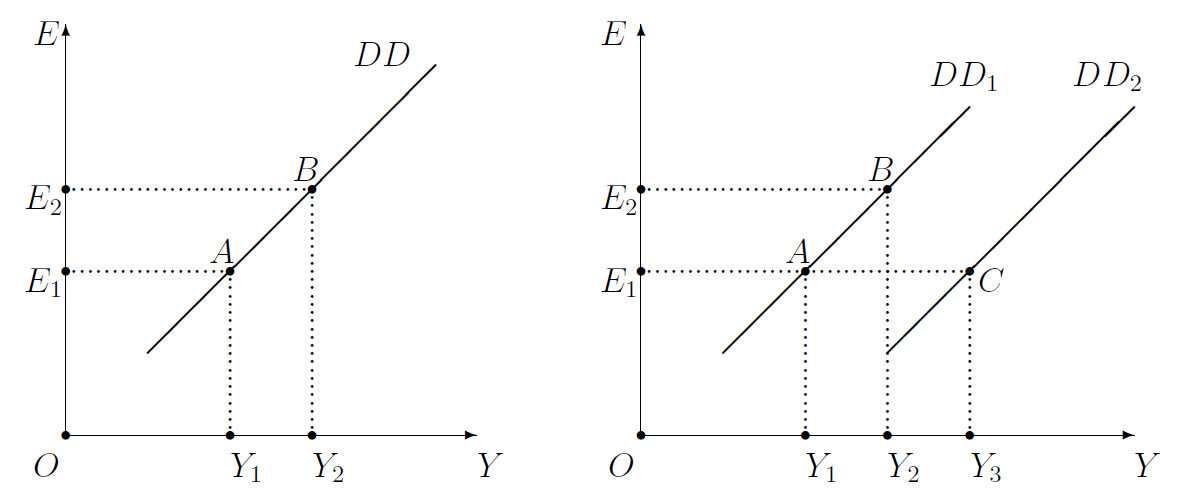
\includegraphics{images/DD_and_shift.png}

}

\caption{\label{fig-DD}If the exogenous variables \(T\), \(I\), \(G\),
\(P^*\), and \(P\) stay unchanged, for the goods market to be in
equilibrium, any increase in \(E\) must be accompanied by an increase in
\(Y\). This direct relation between the exchange rate and output is
called the \(DD\) curve. The \(DD\) curve will shift to the right if
\(T\downarrow\), \(I\uparrow\), \(G\uparrow\), \(P^*\uparrow\), and
\(P\downarrow\).}

\end{figure}%

\subsection{\texorpdfstring{The \emph{DD} Curve:
shifts}{The DD Curve: shifts}}\label{sec-DD-shifts}

It also follows from the last paragraph of the
Section~\ref{sec-goods-short-temp} that if \(E\) remains unchanged at,
say, \(E_1\) in Figure~\ref{fig-DD}, and if one or more of only these
changes occur---\(T\downarrow\), \(I\uparrow\), \(G\uparrow\),
\(P^*\uparrow\), and \(P\downarrow\)---then output would increase
(\(Y\uparrow\)). In other words, assuming the economy was initially at
the equilibrium outcome represented by point \(A\) in
Figure~\ref{fig-DD}, the new equilibrium would be at a point such as
\(C\), with \(E\) unchanged and \(Y\) higher. And, as the \(DD\) curve
represents all possible equilibrium outcomes, if the equilibrium is no
longer at point \(A\), the \(DD\) curve can no longer be \(DD_1\). As
the equilibrium has moved from \(A\) to \(C\), the \(DD\) curve must
also have moved from \(DD_1\) to \(DD_2\). In other words, we have
established that \emph{the \(DD\) curve will shift to the right if one
or more of only the folowing changes occur---\(T\downarrow\),
\(I\uparrow\), \(G\uparrow\), \(P^*\uparrow\), and \(P\downarrow\)}.

This ends my discussion of the goods market, for the time being. The
\(DD\)-column of Table~\ref{tbl-short-temp} gives a hyper-concise
summary.

\section{Asset Markets}\label{sec-assets-short-temp}

Recall from Section~\ref{sec-UIP} that equilibrium in the foreign
exchange market is represented by the uncovered interest parity
equation, Equation~\ref{eq-UIP-alt}, which is
\begin{equation}\phantomsection\label{eq-UIP-short-temp}{
\fbox{$\displaystyle R=R^*+\frac{E^e_f}{E}-1.$}
}\end{equation}

It follows in a straightforward manner that the interest rate (\(R\))
will remain unchanged if \(R^*\), \(E_f^e\), and \(E\) are unchanged.
And, \(R\) will increase if one or more of only the following changes
occur: \(R^*\uparrow\), \(E_f^e\uparrow\), and \(E\downarrow\).

Also, recall from Section~\ref{sec-summary-moneyeqm} that the money
market is in equilibrium when money supply (\(M\)) is equal to money
demand (\(L(R)\cdot P\cdot Y\)):
\begin{equation}\phantomsection\label{eq-LM-short-temp}{
\fbox{$M=L(R)\cdot P\cdot Y.$}
}\end{equation}

The two equations above can be merged into the following equation
representing simultaneous equilibrium in both the money and foreign
exchange markets:
\begin{equation}\phantomsection\label{eq-assets-short-temp}{
M=L\left(R^*+\frac{E^e_f}{E}-1\right)\cdot P\cdot Y.
}\end{equation}

\begin{figure}

\centering{

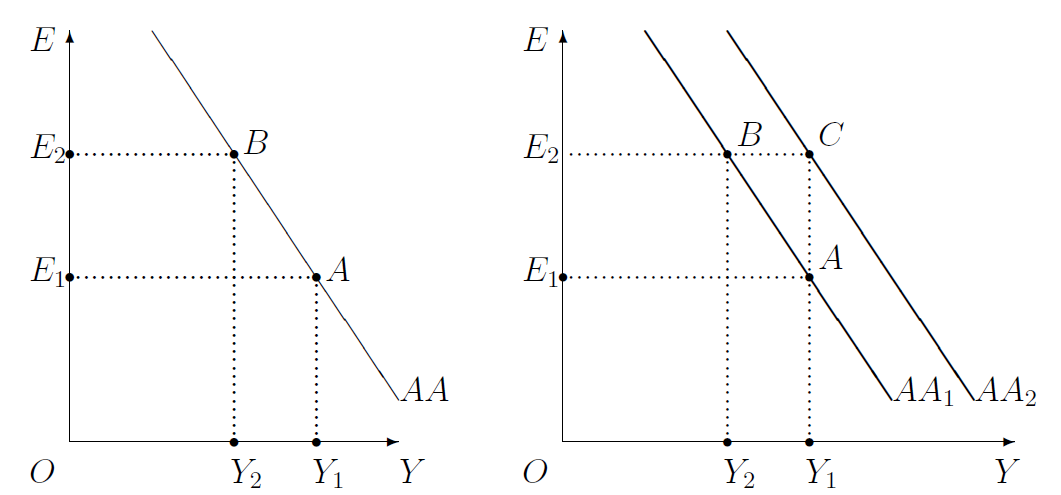
\includegraphics{images/AA_and_shift.png}

}

\caption{\label{fig-AA}For the asset markets to be in equilibrium, if
the exogenous variables \(M\), \(R^*\), \(E_f^e\), and \(P\) stay
unchanged, any increase in \(E\) must be accompanied by a decrease in
\(Y\). This inverse relation between the exchange rate and output is
called the \(AA\) curve. The \(AA\) curve will shift to the right if
\(M\uparrow\), \(P\downarrow\), \(R^*\uparrow\), or \(E_f^e\uparrow\).}

\end{figure}%

\subsection{\texorpdfstring{The \emph{AA} Curve:
slope}{The AA Curve: slope}}\label{sec-AA}

The equation above has two endogenous variables (\(E\) and \(Y\)) and
four exogenous variables (\(M\), \(R^*\), \(E_f^e\), and \(P\)). Suppose
the magnitudes of the exogenous variables are known. Further, suppose
the asset markets are in equilibrium---that is,
Equation~\ref{eq-assets-short-temp} is satisfied---for the values
\(E=E_1\) and \(Y=Y_1\). Would this pair of values for \(E\) and \(Y\)
be the only such pair at which Equation~\ref{eq-assets-short-temp} is
satisfied? Certainly not: there are many others.

If \(R^*\) and \(E_f^e\) stay unchanged and the value of the foreign
currency increases (\(E\uparrow\)), Equation~\ref{eq-UIP-short-temp}
implies that the interest rate must decrease (\(R\downarrow\)). And, we
know from Section~\ref{sec-mdemanddet2}, that this must increase
people's desire for liquidity (\(L(R)\uparrow\)): when the interest rate
decreases people get rid of some of their interest-paying assets (such
as bonds) and hold on to non-interest-paying cash instead. Now, note
that Equation~\ref{eq-LM-short-temp} implies \(Y=M/(L(R)\cdot P)\). As
both \(M\) and \(P\) are unchanged and \(L(R)\) has increased, \(Y\)
must decrease if the asset markets are to remain in equilibrium.
Therefore, we see that, \emph{if the exogenous variables (\(M\),
\(R^*\), \(E_f^e\), and \(P\)) are unchanged, and if the asset markets
are in equilibrium when \(E=E_1\) and \(Y=Y_1\), then the asset markets
will also be in equilibrium for some higher value of \(E\)---such as
\(E=E_2\) in Figure~\ref{fig-AA} ---and some lower value of \(Y\)---such
as \(Y=Y_2\) in Figure~\ref{fig-AA}.}

That is, if initially the asset markets are in equilibrium and \(E=E_1\)
and \(Y=Y_1\) as in point \(A\) in Figure~\ref{fig-AA}, this will not be
the only asset markets equilibrium outcome. Assuming \(M\), \(R^*\),
\(E_f^e\), and \(P\) are fixed, there will exist other equilibrium in
which \(E=E_2\) and \(Y=Y_2\) as in point \(B\). \emph{The collection of
all such outcomes that keep the asset markets in equilibrium is the
\(AA\) curve. As there is an inverse relation between the values of
\(E\) and \(Y\) that keep the asset markets in equilibrium when \(M\),
\(R^*\), \(E_f^e\), and \(P\) are fixed, the \(AA\) curve is
downward-sloping}, as in Figure~\ref{fig-AA}.\footnote{Recall from
  Theorem~\ref{thm-eqnno} that if the number of endogenous variables
  exceeds the number of equations, the equations have many solutions.
  Here, we are dealing with \emph{one}
  equation---Equation~\ref{eq-assets-short-temp} ---that has \emph{two}
  endogenous variables, \(Y\) and \(E\). Therefore, it should not be a
  surprise that there are many pairs of values for \(Y\) and
  \(E\)---such as points \(A\) and \(B\) and, indeed, all the other
  points on the \(AA\) curve in Figure~\ref{fig-AA} ---that all
  represent equilibrium in the asset markets.}

\begin{figure}

\centering{

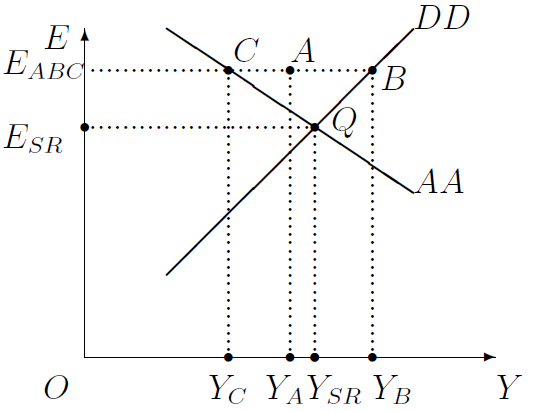
\includegraphics{images/DD_AA_equilibrium.png}

}

\caption{\label{fig-AADD}The short-run equilibrium under flexible
exchange rates is at \(Q\), the intersection of the \(DD\) and \(AA\)
curves.}

\end{figure}%

\subsection{\texorpdfstring{The \emph{AA} Curve:
shifts}{The AA Curve: shifts}}\label{sec-AA-shifts}

Let us return to point \(B\) in Figure~\ref{fig-AA}, where the asset
markets are in equilibrium. Let us consider what would happen if the
money supply increases (\(M\uparrow\)), the other exogenous variables
(\(R^*\), \(E_f^e\), and \(P\)) remain unchanged. Is it possible that at
the new equilibrium the exchange rate is still at \(E=E_2\)? We know
from Equation~\ref{eq-UIP-short-temp} that the interest rate (\(R\))
will not change. Therefore, \(L(R)\) will not change. Therefore, as
Equation~\ref{eq-LM-short-temp} implies \(Y=M/(L(R)\cdot P)\), the
increase in money supply will lead to an increase in output
(\(Y\uparrow\)). That is, when \(M\) increases, there indeed would exist
a new equilibrium such that \(E=E_2\), as before, but with an output
that's higher than before. In other words, the increase in \(M\) pushes
the outcome from \(B\) to \(C\).

Following the same line of reasoning, it can be shown that if domestic
prices fall (\(P\downarrow\)), the other exogenous variables (\(R^*\),
\(E_f^e\), and \(M\)) remain unchanged, and the exchange rate stays
unchanged at \(E=E_2\), then neither \(R\) nor \(L(R)\) will change,
and, consequently, output will increase (\(Y\uparrow\)).

Next, what would happen if the foreign interest rate increases
(\(R^*\uparrow\)), the other exogenous variables (\(M\), \(E_f^e\), and
\(P\)) remain unchanged, and the exchange rate also stays unchanged at
\(E=E_2\). We know from Equation~\ref{eq-UIP-short-temp} that the
interest rate must increase (\(R\uparrow\)). Therefore, as we saw in the
opening paragraph of this section, the people's desire for liquidity
must decrease (\(L(R)\downarrow\)). Therefore, as \(Y=M/(L(R)\cdot P)\),
it follows that output must increase (\(Y\uparrow\)).

The previous paragraph could be repeated word-for-word, but with \(R^*\)
and \(E_f^e\) changing places, to establish that an increase in the
current expectation of the future value of the foreign currency
(\(E_f^e\uparrow\)) must also lead to an increase in output
(\(Y\uparrow\)), assuming \(M\), \(R^*\), \(P\), and \(E\) are
unchanged.

In short, if \(E\) stays unchanged, then, for the asset markets to
remain in equilibrium, \(Y\) must increase if some subset of the
following ceteris paribus changes occurs: \(M\uparrow\),
\(P\downarrow\), \(R^*\uparrow\), and \(E_f^e\uparrow\). In other words,
assuming the economy is initially at an equilibrium outcome represented
by point \(B\) in Figure~\ref{fig-AA}, the new equilibrium would be at a
point such as \(C\). And, as the \(AA\) curve represents all possible
asset markets equilibrium outcomes, if the equilibrium is no longer at
point \(B\), the \(AA\) curve can no longer be \(AA_1\). As the
equilibrium has moved from \(B\) to \(C\), the \(AA\) curve must also
have moved from \(AA_1\) to \(AA_2\). In other words, we have
established that \emph{the \(AA\) curve will shift to the right if one
or more of only the following changes occur---\(M\uparrow\),
\(P\downarrow\), \(R^*\uparrow\), and \(E_f^e\uparrow\)}. These effects
are summarized in the \(AA\)-column of Table~\ref{tbl-short-temp}.

\section{Short-Run Equilibrium}\label{sec-eqm-short-temp}

A crucial feature of the analysis presented here is the assumption that
all three markets---goods, money, and foreign exchange---must be in
equilibrium simultaneously. Therefore, point \(A\) in
Figure~\ref{fig-AADD} cannot represent equilbrium because none of our
three markets are in equilibrium when \(E=E_{ABC}\) and \(Y=Y_A\). Point
\(A\) lies neither on the \(DD\) curve, which includes all outcomes that
represent equilibrium in the goods market, nor on the \(AA\) curve,
which includes all outcomes that represent equilibrium in the asset
markets, meaning the money and foreign exchange markets.

Similarly, neither \(B\) nor \(C\) in Figure~\ref{fig-AADD} can be the
short-run equilibrium. At \(B\), which is on the \(DD\) curve but not on
the \(AA\) curve, the goods market is in equilibrium, but not the asset
markets. At \(C\), the asset markets are in equilibrium but the goods
market is not.

It is only at \(Q\)---that is, where the \(DD\) and \(AA\) curves
intersect---that all three markets are in equilibrium. In other words,
only when the exchange rate is \(E=E_{SR}\) and real GDP is \(Y=Y_{SR}\)
does short-run equilibrium prevail. Figure~\ref{fig-AADD} therefore
shows that, \emph{if an economy's \(DD\) and \(AA\) curves are known,
their intersection determines the short-run equilibrium levels of the
exchange rate and real income}.

\begin{figure}

\centering{

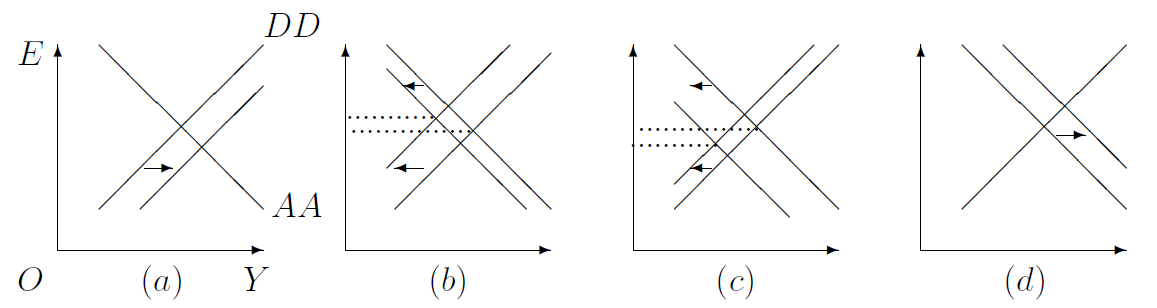
\includegraphics{images/AA_DD_shift.png}

}

\caption{\label{fig-AADD-shifts}Short-run equilibrium under flexible
exchange rates. In panel (a), \(Y\uparrow\) and \(E\downarrow\). In
panel (d), \(Y\uparrow\) and \(E\uparrow\). Panels (b) and (c) show why
the effect of an increase in the domestic price level (\(P\uparrow\)),
which shifts both the \(DD\) and \(AA\) curves to the left, has a
negative effect on output and an ambiguous effect on the exchange rate.
In panel (b), \(DD\) shifts a lot more than \(AA\) and, as a result,
\(E\uparrow\). In panel (c), \(DD\) shifts a lot less than \(AA\) and,
as a result, \(E\downarrow\).}

\end{figure}%

\section{Predictions}\label{sec-short-temp-preds}

We are now close to working out the full short-run consequences of
temporary changes in our exogenous variables. We can now apply (a) our
understanding that the intersection of the \(DD\) and \(AA\) curves
determines the equilibrium values of \(Y\) and \(E\), and (b) our
knowledge of how changes in certain exogenous variables can shift the
\(DD\) and \(AA\) curves, to make predictions about the effects of those
exogenous changes on all our endogenous variables, including \(Y\) and
\(E\).

\subsection{Fiscal Policy}\label{sec-fiscal-short-temp}

Let us begin by analysing the effects of expansionary fiscal policy,
which refers to either an increase in government spending
(\(G\uparrow\)) or a cut in taxes (\(T\downarrow\)) or both. We know
from Section~\ref{sec-DD-shifts} and Section~\ref{sec-AA-shifts} that,
as a result of these changes in fiscal policy, the \(DD\) curve will
shift to the right and the \(AA\) curve will be unaffected. Therefore,
the effects of expansionary fiscal policy can be shown by panel (a) of
Figure~\ref{fig-AADD-shifts}. It follows that, real income will rise
(\(Y\uparrow\)) and the domestic currency will appreciate
(\(E\downarrow\)).

Therefore, disposable income must increase (\(Y-T\uparrow\)). And,
therefore, consumption spending must increase (\(C=C(Y-T)\uparrow\)).

Expansionary fiscal policy cannot affect the domestic and foreign price
levels (\(P\) and \(P^*\)), which are exogenous. Therefore, the decrease
in \(E\) implies a decrease in the real exchange rate
(\(q\equiv E\cdot P^*/P\downarrow\)). The decrease in the real exchange
rate, which implies that foreign goods have become relatively cheaper,
and the increase in disposable income, which leads to more imports, must
both lead to a decrease in net exports
(\(NX=NX(q, Y-T)\downarrow\)).\footnote{See
  Section~\ref{sec-summary-nxp} for more on the factors that drive a
  country's net exports.}

Finally, note that expansionary fiscal policy cannot affect \(R^*\) and
\(E_f^e\), which are exogenous. This, plus the decrease in \(E\),
together imply, as we saw in Section~\ref{sec-assets-short-temp}, that
the domestic interest rate must increase (\(R\uparrow\)).

The reader can verify that the effects of an increase in business
investment (\(I\uparrow\)) are identical to the effects of an increase
in government spending.

To summarize, \emph{if only some subset of these exogenous
changes---\(I\uparrow\), \(G\uparrow\), \(T\downarrow\)---occur, then
\(Y\uparrow\), \(E\downarrow\), \(C\uparrow\), \(NX\downarrow\),
\(q\downarrow\), and \(R\uparrow\)}, as shown in the rows for \(I\),
\(G\), and \(T\) in Table~\ref{tbl-short-temp}.

Note that these results provide an intellectual basis for the use of
expansionary fiscal policy during a recession. Cutting government
spending and raising taxes may represent a rare and admirable sense of
responsibility and restraint in a government, but such otherwise
praiseworthy behavior may not be a good idea when an economy is facing
short-run trouble.

\subsection{Foreign Price Level}\label{sec-pstar-short-temp}

The effects of an increase in foreign prices (\(P^*\uparrow\)) are also
shown by panel (a) of Figure~\ref{fig-AADD-shifts}. Specifically, we
know from Section~\ref{sec-DD-shifts}\} and Section~\ref{sec-AA-shifts}
or from the \(DD\) and \(AA\) columns of Table~\ref{tbl-short-temp} that
the \(DD\) curve shifts right and the \(AA\) curve is unaffected.
Therefore, \(Y\uparrow\) and \(E\downarrow\), as they did under
expansionary fiscal policy. As taxes, which are exogenous, are
unaffected, \(Y-T\uparrow\), which further implies \(C=C(Y-T)\uparrow\).

We know from Section~\ref{sec-consumption} that when disposable income
increases, consumption increases, but by a smaller amount. Therefore,
\(Y-T-C\) must increase, which implies that \(Y-C\) must increase when
\(P^*\) increases, as the exogenous \(T\) is unaffected. Now recall that
the goods market's equilibrium condition, \(Y=C+I+G+NX\), implies
\(NX=Y-C-I-G\). As the rise in the foreign price level (a) cannot affect
\(I\) and \(G\), which are exogenous, and (b) leads to an increase in
\(Y-C\), we can conclude that net exports must increase
(\(NX\uparrow\)).

We have just seen that when \(P^*\) increases, \(NX\) and \(Y-T\) both
increase. Now recall from Section~\ref{sec-summary-nxp} that net exports
(\(NX=NX(q, Y-T)\)) are directly related to \(q\) and \emph{inversely
related} to \(Y-T\). Given that \(Y-T\) has increased, how could \(NX\)
have increased? The only possible explanation is that the real exchange
rate must have increased, and to such an extent that \(NX\) increased in
spite of the increase in \(Y-T\).

Finally, note that higher foreign prices cannot affect \(R^*\) and
\(E_f^e\), which are exogenous. This, plus the decrease in \(E\),
together imply, as we saw in Section~\ref{sec-assets-short-temp}, that
the domestic interest rate must increase (\(R\uparrow\)).

To summarize, \emph{if there is a ceteris paribus increase in \(P^*\),
then \(E\downarrow\), \(Y\uparrow\), \(C\uparrow\), \(NX\uparrow\),
\(q\uparrow\), and \(R\uparrow\)}. These ceteris paribus effects are
shown in the \(P^*\)-row of Table~\ref{tbl-short-temp}.

\subsection{The Interest Rate}\label{sec-rstar-efe-short-temp}

Now let us consider increases in \(R^*\) or \(E_f^e\) or both. From
Section~\ref{sec-DD-shifts} and Section~\ref{sec-AA-shifts} or from the
\(DD\)- and \(AA\)-columns of Table~\ref{tbl-short-temp}, one can check
that the \(DD\) curve will be unaffected and the \(AA\) curve will shift
to the right. These shifts are shown in panel (d) of
Figure~\ref{fig-AADD-shifts}, which makes clear that real output and the
exchange rate will both increase (\(Y\uparrow\) and \(E\uparrow\)). The
increase in \(E\) and the fact that the exogenous prices, \(P\) and
\(P^*\), are unaffected by changes in \(R^*\) and/or \(E_f^e\), together
imply that the real exchange rate must have increased
(\(q\equiv E\cdot P^*/P\uparrow\)). And, the increase in output must
lead to an increase in consumption (\(C=C(Y-T)\uparrow\)), as taxes,
which are exogenous, are unaffected by \(R^*\) or \(E_f^e\).

Moreover, as we saw a few paragraphs ago, \(Y-C\) increases when \(Y\)
increases and \(T\) is unchanged. Therefore, net exports, which we saw a
few paragraphs back are given by \(NX=Y-C-I-G\), must increase.

Now recall the money market's equilibrium condition is given by
Equation~\ref{eq-LM-short-temp} above or \(M=L(R)\cdot P\cdot Y\). This
implies \(L(R)=M/(P\cdot Y)\). As \(M\) and \(P\), which are exogenous,
are unchanged, and \(Y\) has increased, it follows that \(L(R)\) has
decreased. But we know from Section~\ref{sec-mdemanddet2} that \(L(R)\)
is inversely related to \(R\): when interest rates are high, people do
not want to hang on to liquid cash; they'd rather buy interest-paying
bonds. Therefore, the decrease in \(L(R)\) implies that \(R\) has
increased.

To summarize, \emph{if there is a ceteris paribus increase in \(R^*\) or
in \(E_f^e\), then \(E\uparrow\), \(Y\uparrow\), \(C\uparrow\),
\(NX\uparrow\), \(q\uparrow\), and \(R\uparrow\)}. These ceteris paribus
effects are shown in the \(R^*\)- and \(E_f^e\)-rows of
Table~\ref{tbl-short-temp} as a long row of plus (\(+\)) signs.

\subsection{Monetary Stimulus}\label{sec-money-short-temp}

Recall that a nation's central bank can run the printing presses at any
time, and use the newly printed cash to buy financial assets such as
government bonds from John or Jane Q. Public, as a result of which there
would be a quick increase in \(M\). What would be the short run effects
of a temporary increase in the quantity of money in circulation?

The first two paragraphs of the previous section will work just fine if
all mentions of \(R^*\) or \(E_f^e\) are replaced by \(M\). Therefore,
it is easy to check that \(Y\), \(C\), \(NX\), \(q\), and \(E\) will all
increase as a result of an increase in the quantity of money.

The only difference is that increases in \(R^*\) or \(E_f^e\) lead to
higher domestic interest rates whereas an increase in \(M\) leads to
lower domestic interest rates (\(R\downarrow\)). To see why, recall from
Equation~\ref{eq-UIP-short-temp} that \(R=R^*+(E^e_f/E)-1\). An increase
in \(M\) depreciates the domestic currency (\(E\uparrow\)) and has no
effect on other exogenous variables such as \(R^*\) and \(E_f^e\).
Therefore, it follows that the domestic interest rate decreases.

To summarize, \emph{if a nation's money supply increases---and all other
exogenous variables remain unchanged---then \(Y\), \(C\), \(NX\), \(q\),
and \(E\) will all increase, and \(R\) will decrease}. This is shown in
the \(M\)-row of Table~\ref{tbl-short-temp}.

The direct effect of \(M\) on \(Y\) is a hugely important result that is
the intellectual basis of the argument in favor of expansionary monetary
policy in a recession. Indeed, it is now standard practice for central
banks to boost the money supply whenever a recession hits.

\subsection{The Domestic Price Level}\label{sec-p-short-temp}

Finally, we need to work out how our endogenous variables respond to an
increase in the domestic price level. (I have saved the toughest nut for
the last!)

A quick glance at Section~\ref{sec-DD-shifts} and
Section~\ref{sec-AA-shifts} or at the \(DD\) and \(AA\) columns of
Table~\ref{tbl-short-temp} shows that both the \(DD\) and \(AA\) curves
must shift leftward when \(P\) increases. These shifts are portrayed by
panels (b) and (c) in Figure~\ref{fig-AADD-shifts}. It is clear that
output decreases (\(Y\downarrow\)).

But the effect on the exchange rate is \emph{ambiguous}: \(E\) increases
in panel (b), in which \(DD\) shifts more than \(AA\), but decreases in
panel (c) in which \(DD\) shifts less than \(AA\). In other words,
although an increase in the domestic price level affects the equilibrium
outcome in all three markets, if the effect on the goods market is very
strong compared to the effects on the money and foreign currency
markets, then the value of the foreign currency increases. On the other
hand, if the effect on the asset markets is stronger, then the exchange
rate decreases.

Also, recall from Equation~\ref{eq-UIP-short-temp} that
\(R=R^*+(E^e_f/E)-1\). As an increase in \(P\) cannot affect other
exogenous variables such as \(R^*\) and \(E_f^e\), and as the effect on
\(E\) is ambiguous, the effect on the domestic interest rate must be
ambiguous as well.

We have seen several times already that any change in \(Y\) leads to
similar changes in \(C\) and \(Y-C\), provided taxes are unaffected.
Therefore, as an increase in \(P\) cannot affect other exogenous
variables such as \(T\), the decrease in \(Y\) that we saw two
paragraphs back must lead to decreases in \(C\) and \(Y-C\). We have
also seen on several occasions above that the goods market's equilibrium
condition \(Y=C+I+G+NX\) implies \(NX=Y-C-I-G\). Therefore, the decrease
in \(Y-C\) implies a decrease in net exports as well, given that \(I\)
and \(G\), which are exogenous, are unaffected.

Note that when \(P\) increases, \(NX\) and \(Y-T\) both decrease. Now
recall from Section~\ref{sec-summary-nxp} that net exports
(\(NX=NX(q, Y-T)\)) are directly related to \(q\) and inversely related
to \(Y-T\). Given that \(Y-T\) has decreased, how on earth could \(NX\)
have decreased also? The only possible explanation is that the real
exchange rate must have decreased, and decreased to such an extent that
\(NX\) decreased in spite of the decrease in \(Y-T\).\footnote{Alert
  readers will notice that I have used this line of reasoning before to
  deduce the behavior of the real exchange rate whenever disposable
  income and net exports move in the \emph{same} direction. Disposable
  income is supposed to have an \emph{inverse} effect on net exports.
  Therefore, when these two variables move together, it must be the
  doing of the real exchange rate. And, as the real exchange rate is the
  relative price of foreign goods, it has a \emph{direct} effect on net
  exports. Therefore, if the real exchange is reversing the effect of
  disposable income on net exports, it must have changed in the same
  direction as disposable income. For instance, if \(Y-T\) and \(NX\)
  both decrease, then \(q\) must also have decreased.}

To summarize, \emph{if the domestic price level increases and all other
exogenous variables stay unchanged, then \(Y\), \(C\), \(NX\), and \(q\)
must all decrease. The effects on \(E\) and \(R\) are ambiguous}.

This completes my analysis of the short-run effects of temporary changes
in exogenous variables in an economy that has flexible exchange rates.
The results are summarized in Table~\ref{tbl-short-temp}.

\begin{table}

\caption{\label{tbl-short-temp}\textbf{Macroeconomic Behavior under
Flexible Exchange Rates in the Short Run: temporary changes.} All
variables named in the first column are exogenous and all variables
listed in the first row are endogenous. Each cell in the table---except
those in the \(DD\) and \(AA\) columns---shows the relation between the
exogenous variable and the endogenous variable aligned with the cell.
The +/?/- symbols denote a direct/ambiguous/inverse relation. A blank
cell denotes that there is no relation. Each cell in the \(DD\) and
\(AA\) columns shows how the two curves shift, if at all, when the
exogenous variable aligned with that cell \emph{increases}.}

\centering{

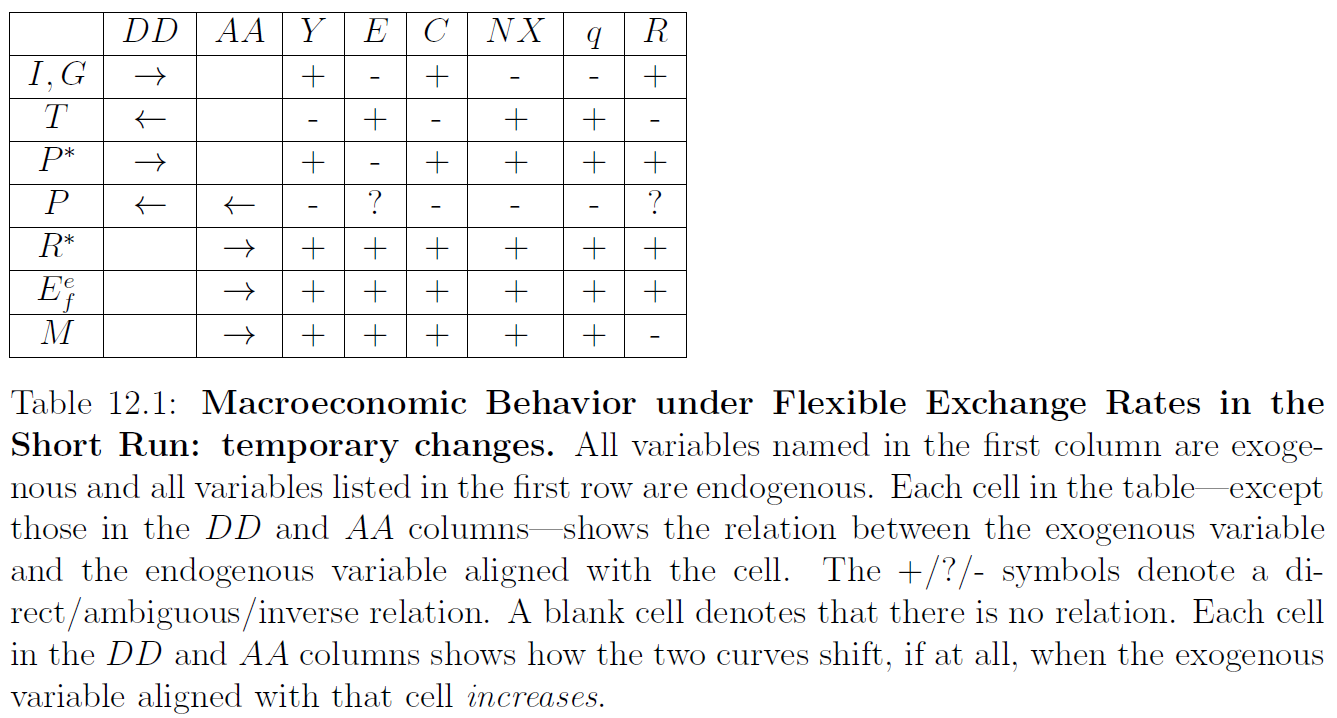
\includegraphics{images/short_flex_temporary.png}

}

\end{table}%

\section{Conclusion}\label{sec-conclusion-short-temp}

A country's net exports (or ``trade balance'') is often a controversial
issue. We have seen in other contexts before that contractionary fiscal
policy (\(G\downarrow\) and/or \(T\uparrow\)) consistently leads to
higher net exports. It is, therefore, a relief to see the same result in
this chapter.

Although casual commentators often suggest an increase in tariffs on
imported goods as a way to increase net exports, we have seen in
Chapter~\ref{sec-longreal}\} that tariffs do not affect net exports in
the long run. An increase in tariffs does raise net exports in the short
run under fixed exchange rates, as we saw in the last chapter. This
chapter's analysis shows the same effect is true under flexible exchange
rates as well.

\bookmarksetup{startatroot}

\chapter{Short-Run Predictions: Expectations and Flexible Exchange
Rates}\label{sec-short-perm}

This chapter continues the analysis of the short-run macroeconomic
behavior of an economy that has flexible exchange rates. The questions
that concern us in this chapter share this basic format: If there is a
\emph{permanent} increase in {[}insert the name of any exogenous
variable{]}, what will happen in the short run to {[}insert the name of
any endogenous variable{]}?

Recall that the consequences of \emph{temporary} shocks and
\emph{temporary} policy changes were discussed in the previous chapter.
The reason why it makes sense to analyse temporary and permanent changes
in exogenous variables separately was discussed in the last paragraph of
Section~\ref{sec-sr-expectations} and at the beginning of
Chapter~\ref{sec-short-temp}. The crucial difference is that permanent
changes affect the future---and therefore our expectation of what our
future will be---whereas temporary changes don't.

\section{Fiscal Policy}\label{sec-fiscal-short-perm}

Let us jump right in and try to analyze the short-run effects of a
permanent increase in government spending.

\subsection{The Primary Effect}\label{sec-fiscal-short-perm-primary}

We begin by recalling---from Section~\ref{sec-fiscal-short-temp} or the
\(G\)-row of table Table~\ref{tbl-short-temp} ---the short-run effects
of a \emph{temporary} increase in government spending. The \(DD\) curve,
which represents all pairs of values of real output (\(Y\)) and the
exchange rate (\(E\)) that keep the goods market in equilibrium, shifts
to the right. The \(AA\) curve, which represents all pairs of values of
real output (\(Y\)) and the exchange rate (\(E\)) that keep the money
and foreign currency markets in equilibrium, stays put. As a result,
there are increases in output, consumption, and the interest rate
(\(Y\uparrow\), \(C\uparrow\), \(R\uparrow\)), and decreases in net
exports, the nominal exchange rate, and the real exchange rate
(\(NX\downarrow\), \(E\downarrow\), \(q\downarrow\)).

Needless to say, these effects are temporary. A temporary increase in
government spending will, by definition, soon be reversed. Therefore,
\(G\) will return to its original level. The \(DD\) curve will return to
its original position, and all endogenous variables will return to their
original values.

On the other hand, when the increase in government spending is
permanent, the \(DD\) curve will shift \emph{permanently} to the right.
Therefore, the temporary changes in \(Y\), \(C\), \(R\), \(NX\), \(E\),
and \(q\) that we saw two paragraphs back will now be permanent.

I will call these effects of a permanent increase in government spending
the \emph{primary effect}. The primary effect of a permanent increase in
government spending is the same as the short-run effect of a temporary
increase in government spending that we saw in the \(G\)-row of table
Table~\ref{tbl-short-temp}.

In general, \emph{the primary short-run effect of a permanent increase
in any given exogenous variable \(X\) on any endogenous variable \(Z\)
is identical to the short-run effect of a temporary increase in \(X\) on
\(Z\), and this effect can be seen in the \(X\)-row and \(Z\)-column of
Table~\ref{tbl-short-temp}.}

\subsection{The Secondary Effect}\label{sec-fiscal-short-perm-scondary}

So far, it looks as if distinguishing between permanent and temporary
changes in an exogenous variable is a waste of time. It looks as if a
permanent increase in \(G\) has the same effects as a temporary increase
in \(G\), except that the effects of former are permanent and the
effects of the latter are temporary.

But actually there's more to the story. A permanent increase in \(G\)
will reduce the long-run equilibrium value of \(E_f\), which will lead
to an immediate decrease in \(E_f^e\), which will have additional
short-run effects of its own (on our endogenous variables).

Feeling dizzy? Let's go over this step by step.

The \(G\)-rows of tables Table~\ref{tbl-real_long} and
Table~\ref{tbl-nominal_long_flex} summarize the long-run effects of a
permanent increase in government spending. Note in particular that the
long-run equilibrium value of the future value of the foreign currency
decreases (\(E_f\downarrow\)). Now recall from
Section~\ref{sec-shortana} that in short-run analysis it is assumed that
the expected value of \(E_f\) is equal to its long-run equilibrium
value: that is, \(E_f^e=E_{fLR}\). Therefore, it follows that, as soon
as the permanent increase in government spending occurs, people will
realize that \(E_f\) will eventually fall, and, consequently, they will
revise downward their expectation of the future value of the foreign
currency (\(E_f^e\downarrow\)).

Will this decrease in \(E_f^e\) have further effects on our endogenous
variables? Indeed, it will. Recall from
Section~\ref{sec-rstar-efe-short-temp} and the \(E_f^e\)-row of table
Table~\ref{tbl-short-temp} that a temporary decrease in \(E_f^e\) will
temporarily affect various endogenous variables: \(Y\downarrow\),
\(C\downarrow\), \(R\downarrow\), \(NX\downarrow\), \(E\downarrow\), and
\(q\downarrow\). Therefore, a \emph{permanent} decrease in \(E_f^e\)
will have the same effects, only this time the effects will be
\emph{permanent}.

I will call these effects of a permanent increase in government spending
the \emph{secondary effect}, because it works indirectly by influencing
people's expectations (\(E_f^e\)).

In general, the indirect short-run effect of a permanent increase in any
given exogenous variable \(X\) on any endogenous variable \(Z\) can be
deduced as follows: First, look at the \(X\)-row and \(E_f\)-column of
Table~\ref{tbl-nominal_long_flex} to see whether the long-run
equilibrium value of \(E_f\) will increase or decrease if \(X\)
increases.\footnote{Actually, \(E_f^e\) may stay unchanged. It may even
  be that the effect of \(X\) on \(E_f\) is ambiguous. I am just trying
  to keep the discussion simple.} Second, look at the \(E_f^e\)-row of
table Table~\ref{tbl-short-temp} to see whether the endogenous variable
\(Z\) will increase or decrease. In this way, we can deduce the
secondary effect of \(X\) on \(Z\).

Actually, the process of figuring out the secondary effect of exogenous
variable \(X\) on endogenous variable \(Z\) can be further simplified.
The second step in the last paragraph is actually unnecessary. To see
why, note that the \(E_f^e\)-row of table Table~\ref{tbl-short-temp} has
all plus (\(+\)) signs, indicating that any change in \(E_f^e\) causes
\emph{all} the relevant endogenous variables to change in the same
direction. Therefore, \emph{if you know that an increase in \(X\) leads
to an increase (respectively, a decrease) in \(E_f^e\), you can
immediately conclude that the secondary effect of an increase in \(X\)
will lead to an increase (respectively, a decrease) in all endogenous
variables including \(Z\)}.

\begin{table}

\caption{\label{tbl-short-perm}\textbf{Short-Run Behavior under Flexible
Exchange Rates: permanent changes.} All variables named in the first
column are exogenous and all variables listed in the first row are
endogenous. Each cell in the table shows the relation between the
exogenous variable and the endogenous variable aligned with the cell.
The +/?/- symbols denote a direct/ambiguous/inverse relation. A blank
cell denotes that there is no relation.}

\centering{

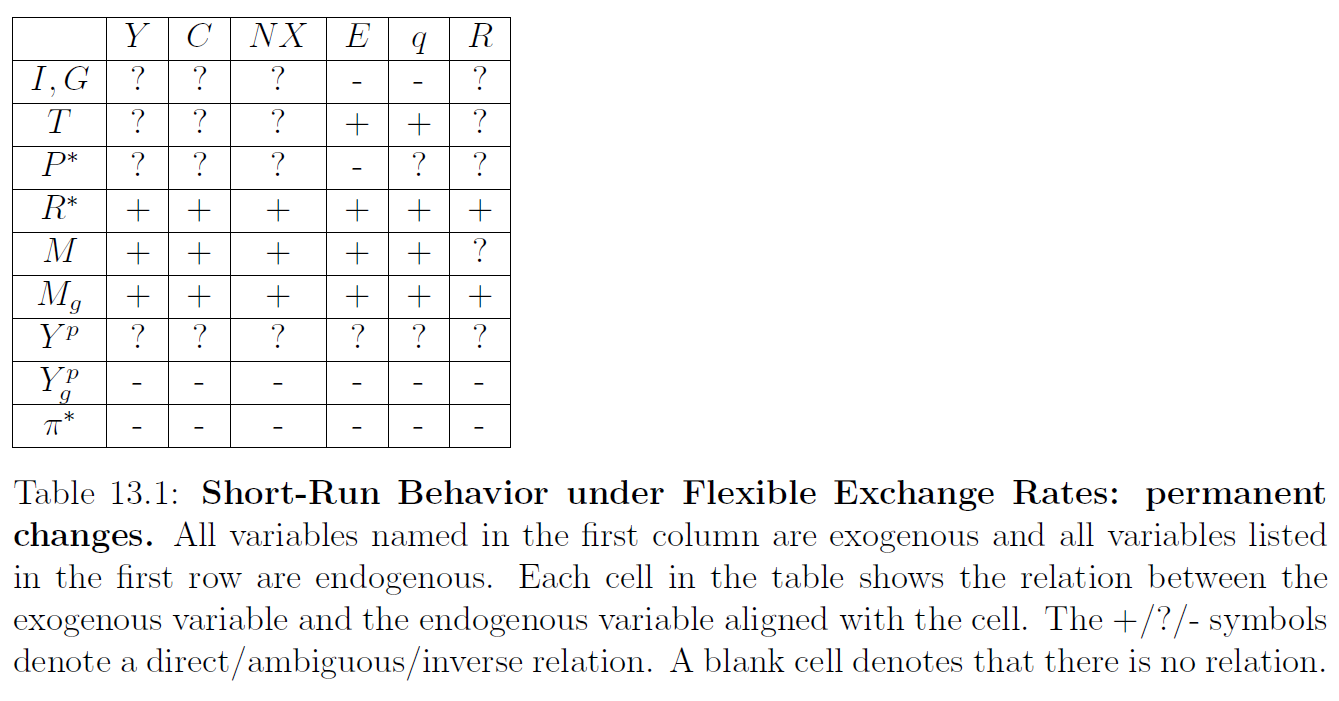
\includegraphics{images/short_flex_permanent.png}

}

\end{table}%

\subsection{The Total Effect}\label{sec-fiscal-short-perm-total}

It is now time to add the \emph{primary} and \emph{secondary} effects of
a permanent increase in government spending and thereby deduce the
\emph{total} effects.

\begin{itemize}
\tightlist
\item
  primary effect of a permanent increase in \(G\) (same as the temporary
  effects in table Table~\ref{tbl-short-temp}): \(Y\uparrow\),
  \(C\uparrow\), \(R\uparrow\), \(NX\downarrow\), \(E\downarrow\),
  \(q\downarrow\)
\item
  effect of a permanent increase in \(G\) on expectations (see
  Table~\ref{tbl-nominal_long_flex}): \(E_f^e\downarrow\)
\item
  secondary effect of a permanent increase in \(G\) (same as the effect
  on \(E_f^e\)): \(Y\downarrow\), \(C\downarrow\), \(R\downarrow\),
  \(NX\downarrow\), \(E\downarrow\), \(q\downarrow\)
\item
  total effect: \(Y?\), \(C?\), \(R?\), \(NX\downarrow\),
  \(E\downarrow\), \(q\downarrow\), where ``\(?\)'' stands for an
  ambiguous effect
\end{itemize}

Note that when the direct and indirect effects go in opposite
directions, the total effect is, unfortunately, ambiguous.

The total effects are summarized in the \(G\)-row of table
Table~\ref{tbl-short-perm}. It is straightforward to check that the
short-run effects of a permanent increase in business investment
(\(I\uparrow\)) are identical, which is why \(G\) and \(I\) share the
same row in table Table~\ref{tbl-short-perm}.

Note that the primary and secondary effects of a permanent increase in
government spending on real output run in opposite directions. The
primary effect leads to higher \(Y\) and the secondary effect leads to
lower \(Y\). As a result, the effect of a permanent fiscal stimulus on
output is weaker than that of a temporary stimulus. Indeed, I cannot
rule out the possibility that the secondary effect may be stronger than
the primary effect, in which case a fiscal stimulus can be
counterproductive and lead to \emph{lower} real output.

\section{More Examples}\label{sec-short-perm-effect-examples}

In general, the short-run effect of a permanent increase in any given
exogenous variable \(X\) on any given endogenous variable \(Z\) can be
deduced as follows:

\begin{itemize}
\tightlist
\item
  The primary short-run effect of a permanent increase in \(X\) is shown
  in the \(X\)-row and \(Z\)-column of table Table~\ref{tbl-short-temp}.
  Make a note of this effect.
\item
  The effect of a permanent increase in \(X\) on \(E_f^e\) is shown in
  the \(X\)-row and \(E_f\)-column of Table~\ref{tbl-nominal_long_flex}.
  Make a note of this effect.
\item
  The secondary short-run effect of a permanent increase in \(X\) on
  \(Z\) is the same as \(X\)'s effect on \(E_f^e\) that we saw in the
  previous step.
\item
  The total short-run effect is the sum of the primary and secondary
  effects. If these two effects are pulling in opposite directions, the
  total effect is ``ambiguous'' or ``\(?\)''.
\end{itemize}

To illustrate, let us consider a permanent increase in money supply
(\(M\)).

\begin{itemize}
\tightlist
\item
  The primary short-run effects of a permanent increase in \(M\) are
  shown in the \(M\)-row of table Table~\ref{tbl-short-temp}:
  \(Y\uparrow\), \(C\uparrow\), \(R\uparrow\), \(NX\uparrow\),
  \(E\uparrow\), \(q\uparrow\)
\item
  The effect of a permanent increase in \(M\) on \(E_f^e\) is shown in
  the \(M\)-row and \(E_f\)-column of Table~\ref{tbl-nominal_long_flex}:
  \(E_f^e\uparrow\)
\item
  The secondary short-run effects of a permanent increase in \(M\) are
  the same as \(M\)'s effect on \(E_f^e\): \(Y\uparrow\), \(C\uparrow\),
  \(R\uparrow\), \(NX\uparrow\), \(E\uparrow\), \(q\uparrow\)
\item
  The total short-run effect is the sum of the primary and secondary
  effects: \(Y\uparrow\), \(C\uparrow\), \(R\uparrow\), \(NX\uparrow\),
  \(E\uparrow\), \(q\uparrow\)
\end{itemize}

This is shown in the \(M\)-row of table Table~\ref{tbl-short-perm}.

Note that the primary effect of monetary policy is reinforced or
strengthened by the secondary effect. This implies that the short-run
impact of a monetary stimulus will be stronger if it is permanent rather
than temporary.

For another example, let us consider the short-run effect of a permanent
increase in the foreign inflation rate (\(\pi^*\uparrow\)).

\begin{itemize}
\tightlist
\item
  There are no primary short-run effects of a permanent increase in
  \(\pi^*\), as table Table~\ref{tbl-short-temp} does not even have a
  \(\pi^*\)-row!
\item
  The effect of a permanent increase in \(\pi^*\) on \(E_f^e\) is shown
  in the \(\pi^*\)-row and \(E_f\)-column of
  Table~\ref{tbl-nominal_long_flex}: \(E_f^e\downarrow\)
\item
  The secondary short-run effects of a permanent increase in \(\pi^*\)
  are the same as \(\pi^*\)'s effect on \(E_f^e\): \(Y\downarrow\),
  \(C\downarrow\), \(R\downarrow\), \(NX\downarrow\), \(E\downarrow\),
  \(q\downarrow\)
\item
  The total short-run effect is the sum of the primary and secondary
  effects: \(Y\downarrow\), \(C\downarrow\), \(R\downarrow\),
  \(NX\downarrow\), \(E\downarrow\), \(q\downarrow\)
\end{itemize}

This is shown in the \(\pi^*\)-row of table Table~\ref{tbl-short-perm}.
Note that, as there is no primary short-run effect of an increase in the
foreign inflation rate, its total short-run effect consists of the
secondary effect of \(\pi^*\) on \(E_f\) and, therefore, on \(E_f^e\).
This is also true for the rows in table Table~\ref{tbl-short-perm} for
\(Y^p\), \(M_g\), and \(Y^p_g\). In the case of \(Y^p\) there is an
additional complication. A quick look at
Table~\ref{tbl-nominal_long_flex} will show that the long-run effect of
an increase in potential output on the future value of the foreign
currency is ambiguous. Therefore, the effect of \(Y^p\) on \(E_f^e\) is
ambiguous. And, therefore, the indirect effects of \(Y^p\) on our
endogenous variables are ambiguous as well.

Using the step-by-step process illustrated in the three examples above
for the \(G\), \(M\), and \(\pi^*\) rows of table
Table~\ref{tbl-short-perm}, the contents of all the other cells can be
verified. I leave that task to the reader.

\section{Conclusion}\label{sec-short-perm-conclusion}

From the point of view of policy making, it is important to note that
the short-run effect of a permanent change in government spending and/or
taxes is weaker than---or, possibly, even the reverse of---a temporary
change. A temporary increase in government spending on, say, the
construction of roads, bridges, etc., or a temporary tax cut stimulates
demand and leads to an increase in output and the creation of new jobs
for the jobless. But there is less reason to be optimistic about the
short-run stimulative effect of a permanent increase in government
spending or a permanent tax cut. A permanent fiscal stimulus will, in
the long run, raise the value of the domestic currency
(\(E_f\downarrow\)). Knowing this, people will revise upward their
expectations about the future value of the domestic currency
(\(E_f^e\downarrow\)), and will do so immediately. This will reduce the
competitiveness of domestic goods---as can be checked from the
\(E_f^e\)-row of table Table~\ref{tbl-short-temp}, \(q\downarrow\),
which implies that foreign goods become relatively cheaper---and lead to
a fall in net exports, lower output, and fewer jobs.

In other words, a permanent fiscal stimulus creates jobs and destroys
jobs at the same time, and the overall effect could go either way.

Of course, a lot depends on the assumption that expectations (\(E_f^e\))
are tightly linked to the long-run equilibrium outcome (\(E_{fLR}\)). I
have assumed that as soon as a permanent increase in government spending
is announced, the people will figure out that \(E_f\) will end up higher
than they had previously thought. As a result, \(E_f^e\) will increase
rightaway. This is at the root of the adverse secondary effect that says
that net exports will fall and, consequently, output will shrink. But
if, in the real world, people do not put two and two together and do not
revise their expectations immediately after the increase in \(G\), then
the adverse secondary effect would not happen, and the fiscal stimulus
will work unobstructed.

A monetary stimulus, in stark contrast, has a stronger effect when it is
permanent. Perhaps a policy lesson that we can take from this chapter is
that a government facing a recession should use a temporary fiscal
stimulus and a permanent monetary stimulus.

\bookmarksetup{startatroot}

\chapter{Special Topic: Currency Crises}\label{sec-crises}

My earlier discussion of the short-run macroeconomic behavior of an open
economy under fixed exchange rates sidestepped the issue of currency
crises. A currency crisis\index{currency crisis} is quite possibly one
of the most dramatic, headline grabbing events in economics. In this
lecture I will discuss why currency crises happen and what can be done
about them.

\section{Inadequate Foreign Currency Reserves}\label{sec-lowreserves}

In a fixed exchange rate system, the nation's central bank stands ready
to buy and/or sell any amount of the domestic currency at a specified
rate called the peg. For example, the U.S. Federal Reserve may announce
that it will buy and sell U.S. dollars at the pegged rate of 1.50
British pounds per dollar. If such an announcement is in fact made, the
market value of the U.S. dollar would immediately become 1.50 pounds per
dollar.\footnote{See Section~\ref{sec-fixexrates} for a refresher.}

If, following such an announcement, people turn up at the Fed's offices
to buy dollars with the pounds they are carrying, the Fed will simply
(i) add those pounds to its reserves of foreign currencies and (ii)
print new dollar bills to pay the people. So, two things happen: the
Fed's \textbf{foreign currency reserves}
\index{foreign currency reserves}, \(R\), increase and the U.S. money
supply, \(M\), increases.

When people appear at the Fed to \emph{sell} dollars for pounds, the
opposite happens: the Fed's pound reserves and the U.S. money supply
both decrease.

So, if exchange rates are fixed, a country's reserves of foreign
currencies, \(R\), and its money supply, \(M\), will either increase
together or decrease together or stay unchanged.

Now, under fixed exchange rates, what are the circumstances in which
\(M\) might decrease? If you look at my earlier discussion of the
short-run behavior of a fixed exchange rate system---especially
Table~\ref{tbl-short_fixed}, which summarizes the main results---you
will notice that \(M\) will decrease if:

\begin{enumerate}
\def\labelenumi{\arabic{enumi}.}
\tightlist
\item
  Either \(i^*\), \(e\) or \(t\) increases
\item
  Or if \(P^*\), \(Y^p\), \(\pi^e\), \(e_g^e\), \(G\), \(c\) or
  \(\theta\) decreases.
\end{enumerate}

When any of these events occur, \(M\) will decline and, as was just
explained, the decline in \(M\) will be accompanied by a decline in
\(R\). (By the way, you can check that many of these effects are also
true in the long run; see Table~\ref{tbl-nominal_long_fix}.)

Let's say that one of the events listed above actually happens raising
the possibility of a decline in \(M\)---and, therefore, in \(R\). In
other words, people are expected to start arriving at the Fed to buy
some of the Fed's stash of British pounds. Specifically, let's say that
the people are expected to line up at the Fed's door---not all at once
but, say, over a two month period---to spend one trillion dollars to buy
pounds at the Fed's announced rate of 1.50 pounds per dollar. So, if the
process reaches its expected completion, one trillion dollars will
disappear from people's wallets into the Fed's vaults---meaning that
\(M\) will decline by one trillion dollars---and \(R\), the Fed's pound
reserves, will decline by 1.50 trillion pounds.

But what if the Fed had only 1.00 trillion pounds to begin with?
Clearly, the Fed would run out of pounds before all those who wanted to
buy pounds could do so. Therefore, the Fed will ultimately have to take
back its promise to buy pounds at \$1.50 per pound and, therefore,
abandon its fixed exchange rate system altogether. That is, the Fed will
be forced to switch to a flexible exchange rate system, which entails no
promises of any kind.

The question then is, will the dollar's value increase or decrease when
the fixed exchange rate system ends and the flexible exchange rate
system begins? The answer is simple: the dollar's value will have to
fall when the Fed stops buying dollars with its pound reserves. When the
Fed buys dollars it props up the dollar's value. So when the Fed stops
buying dollars, the demand for and, therefore, the value of the dollar
will decline.

To summarize,

\begin{enumerate}
\def\labelenumi{\arabic{enumi}.}
\tightlist
\item
  if an economy has a fixed exchange rate system and
\item
  if something happens today that is likely to reduce \(M\) and,
  therefore, \(R\) and is also likely to be hard to reverse and
\item
  if it is known that the central bank's foreign currency reserves are
  inadequate,
\end{enumerate}

then an abrupt collapse of the fixed exchange rate system sometime ahead
in the future followed by a sharp decline in the value of the home
country's currency will be widely anticipated.

But if people fear a decline in the dollar's value in two months time,
what would they do?

Fearing a fall in the value of the dollar, people will try to sell the
dollar for pounds while the dollar is still (temporarily) high. But this
will only accelerate the emptying of the central bank's reserves and
hasten the abandonment of the peg. In short, if something happens that
would cause people to sell dollars, then that itself would cause more
people to want to sell dollars.

Let's say that initially people believe that the fixed exchange rate
system would have to be abandoned by the Fed in two months (i.e.,
\emph{eight} weeks) and that the dollar's value would fall at that time.
It would then be rational to want to sell dollars for pounds
\emph{seven} weeks from today. But people will quickly realize that,
therefore, the Fed would run out of pounds not eight weeks from today
but seven weeks from today. In other words, people would expect the
dollar's value to fall seven weeks from today. Realizing this,
individuals would now want to sell their dollars one week earlier, i.e.,
\emph{six} weeks from today. But then people would quickly realize that
since it is advantageous for everybody to do that, the dollar's value
will fall not eight weeks from today but just six weeks from today. And
so on and on. Continuing in this way, we realize that the first whiff of
a \emph{future} currency crisis would cause an \emph{immediate} currency
crisis. There would be a mad dash for the exits as people try, all at
the same time, to sell their dollars to the Fed for pounds. The Fed
would lose all its pounds before it even realized what had happened.

Let's look at the whole process in a slightly different way. Saying that
a sharp decline in \(e\) will be widely anticipated is like saying that
\(e_g^e\) will decrease. And as was discussed earlier, this will add to
the downward pressure on \(M\) and hasten the demise of the fixed
exchange rate system because the added downward pressure on \(M\)
implies an added downward pressure on \(R\), which would lead people to
expect an even quicker exhaustion of the central bank's foreign currency
reserves. But if people accordingly revise their prediction of the
likely date of the death of the fixed exchange rate system, it would
mean a further decline in \(e_g^e\) which would further hasten the
demise of the fixed exchange rate system, and so on.

In short, a currency crisis occurs in two stages. First, something
happens---either \(i^*\), \(e\) or \(t\) increases or \(P^*\), \(Y^p\),
\(\pi^e\), \(e_g^e\) , \(G\), \(c\) or \(\theta\) decreases---that
reduces \(M\) and \(R\). Second, there is a series of declines in
\(e_g^e\) that finish the job off. What is scary is that even the first
stage, in which the currency crisis is born, may consist of a decline in
\(e_g^e\). So, the whole crisis, from beginning to end, may occur simply
because of a possibly baseless fear that the currency's value would
fall. That initially baseless fear could set in motion a self-fulfilling
prophecy that would end up confirming the fear.

\section{Currency Boards}\label{sec-currboard}

What is even scarier is that a currency crisis can occur even if the
central bank has adequate foreign currency reserves, in which case the
fixed exchange rate system is called a \textbf{currency board}
\index{currency board}. To see why, let us return briefly to
Table~\ref{tbl-short_fixed}, the table that summarizes the results for
an economy in the short-run under fixed exchange rates. Note that the
columns for \(M\) and \(Y\) are virtually identical. So, \(M\) and \(Y\)
usually move in the same direction; if something happens that makes
\(M\) decrease it will very likely also make \(Y\) decrease. Now, when
\(Y\) decreases, the country's government, fearful of becoming
unpopular, will be tempted to devalue the currency (that is, it will be
tempted to reduce the pegged value of \(e\)) in order to reverse the
decline in \(Y\). And if a sudden sharp decline in \(e\) is widely
anticipated, a currency crisis will develop just as before: \(e_g^e\)
will go down making a bad situation worse and, as we saw earlier, this
itself might precipitate a currency crisis.

So, the possibility that the central bank will abandon fixed exchange
rates either because it has inadequate reserves or because it will have
to do something about the declining \(Y\), could precipitate a currency
crisis.

\section{Dealing with a Currency Crisis}\label{sec-cure}

Table~\ref{tbl-short_fixed} suggests several ways of dealing with an
unfolding currency crisis: increase government spending, \(G\), cut
taxes, \(t\), or raise tariffs, \(\theta\), on imported goods. As the
table shows, if any or all of these things are done, \(M\) and,
therefore, \(R\) will increase, thereby reversing the initial decrease
in \(M\) that precipitated the crisis.

The problem with this strategy is that the crisis is likely to happen
much too quickly for \(G\), \(t\) and \(\theta\) to have any timely
effect. Besides, if the government is to cut taxes and increase spending
at the same time, it would have to borrow money from private citizens
and such borrowing may be prohibitively expensive, particularly since it
is being done in the middle of a currency crisis. And as for tariffs,
the effect on \(M\) is likely to be weak.

So, what's to be done?

One way out is to get wealthy foreign governments or the International
Monetary Fund\index{International Monetary Fund} to come to the crisis
country's aid with a generous line of credit. Suppose people have begun
arriving at the Fed to buy British pounds. If it transpires that the Fed
has an inadequate stock of pounds, the orderly process of people lining
up to buy pounds could quickly turn into a full-fledged currency crisis,
as we saw earlier. But if some wealthy foreign government or the IMF
steps in with a large loan of British pounds for the Fed, the fear that
the fed will run out of pounds will go away and, therefore, the currency
crisis itself will go away.

Of course, the Fed will have to pay those borrowed British pounds back
eventually. Therefore, if nothing is done between now and `eventually',
the crisis will return. Consequently, all that foreign loans can do is
buy the U.S. some time. If the breathing space thus obtained is used to
reverse the decline in \(M\)---by increasing \(G\) and reducing \(t\),
as was discussed in the first paragraph of this section---then the
crisis will truly end. Emergency infusions of foreign currency reserves
combined with necessary changes in domestic policy can effectively bring
a currency crisis to an end.

However, all this, while fine in theory, is very tricky to pull off
right in the middle of an actual currency crisis. Therefore, we need to
focus on prevention.

\section{Preventing a Currency Crisis}\label{sec-preven}

What can be done to prevent a currency crisis? There are three
possibilities.

\begin{enumerate}
\def\labelenumi{\arabic{enumi}.}
\item
  Don't have a fixed exchange rate system in the first place. Have
  flexible exchange rates instead. However, the downside of a flexible
  exchange rate system is that the uncertainty associated with the
  exchange rate fluctuations that might follow would reduce trade and,
  therefore, hurt the country's economic health.
\item
  Make sure the central bank piles up enough foreign exchange reserves
  so that it will never run out---that is, adopt the currency board
  system. For example, suppose 2 trillion dollars have been printed so
  far. If the Fed announces a peg of 1.50 pounds per dollar and if the
  Fed has 3 trillion British pounds in its reserves, then it will never
  run out of pounds: Not even if every single dollar out there is sold
  to the Fed for pounds. However, this system---the currency board---is
  not foolproof. As was pointed out in Section~\ref{sec-currboard}, a
  currency crisis can occur even when there are enough reserves.
\item
  Join up with other countries with which you wanted to have fixed
  exchange rates and jointly decide to adopt a single currency for all
  countries. This system---called a \textbf{currency union}
  \index{currency union}---would allow all the advantages of a fixed
  exchange rate system without the fear of periodic currency crises.
\end{enumerate}

The most important example of the currency union solution to the problem
of currency crises is the European Monetary
Union\index{European Monetary Union} and the birth of the Euro and
that's our next topic.

\bookmarksetup{startatroot}

\chapter{International Macroeconomics:
Summary}\label{sec-intmac_summary_tables}

\section{Short-Run Equations}

\[
1=c\cdot (1-t)+IN(i^*-e_g^e-\pi^e)+\frac{G}{Y}+EX\left(\frac{e\cdot P}{P^*}\right)\cdot \frac{Y^p}{Y}-IM\left(\frac{e\cdot P}{P^*},\theta\right)
\]

\[
\frac{M}{P}=L(i^*-e_g^e)\cdot Y
\]

\section{Short-Run Predictions for Flexible Exchange Rates}

\begin{table}
\begin{tabular}{*{11}{|c}|}
\hline
%\multicolumn{11}{|c|}{\textbf{Flexible Exchange Rates and Short Run}}\\ \hline
    &$Y$    &$C$    &$I$    &$NXP$ &$EXP$   &IMP    &$i$    &$r^e$  &$e$    &$\epsilon$  \\ \hline
$G$ &   &   &   &-  &-      &+  &   &   &+              &+\\ \hline
$t$ &   &-  &   &+  &+      &-  &   &   &-              &-\\ \hline
$c$ &   &+  &   &-  &-      &+  &   &   &+              &+\\ \hline
$i^*$   &+  &+  &?  &?  &+      &?  &+  &+  &-              &-\\ \hline
$\theta$ &  &   &   &   &-      &-  &   &   &+              &+\\ \hline
$Y^p$   &   &   &   &   &+      &+  &   &   &+              &+\\ \hline
$P^*$   &   &   &   &   &       &   &   &   &+              & \\ \hline
$P$ &-  &-  &-  &?  &-      &?  &   &   &?              &+\\ \hline
$\pi^e$ &   &   &+  &-  &-      &+  &   &-  &+              &+\\ \hline
$e^e_g$ &-  &-  &?  &?  &-      &?  &-  &-  &+              &+\\ \hline
$M$ &+  &+  &+  &?  &+      &?  &   &   &-              &- \\ \hline

\end{tabular}

\caption{Short-Run Predictions for Flexible Exchange Rates}

\end{table}

\section{Short-Run Predictions for Fixed Exchange Rates}

\begin{table}

\begin{tabular}
{*{10}{|c}|}
\hline
%\multicolumn{10}{c}{\textbf{Fixed Exchange Rates and Short Run}}\\ \hline

        &$Y$    &$C$    &$I$    &$NXP$  &$EXP$  &$IMP$  &$i$    &$r^e$ &$M$\\ \hline
$G$     &+  &+  &+  &-  &   &+  &   &   &+\\ \hline
$t$     &-  &-  &-  &+  &   &-  &   &   &-\\ \hline
$c$     &+  &+  &+  &-  &   &+  &   &   &+\\ \hline
$i^*$       &-  &-  &-  &+  &   &-  &+  &+  &-\\ \hline
$\theta$    &+  &+  &+  &?  &   &?  &   &   &+\\ \hline
$Y^p$       &+  &+  &+  &?  &+  &+  &   &   &+\\ \hline
$P^*$       &+  &+  &+  &?  &+  &?  &   &   &+\\ \hline
$P$     &-  &-  &-  &?  &-  &?  &   &   &?\\ \hline
$\pi^e$ &+  &+  &+  &-  &   &+  &   &-  &+\\ \hline
$e_g^e$     &+  &+  &+  &-  &   &+  &-  &-  &+\\ \hline
$e$     &-  &-  &-  &?  &-  &?  &   &   &- \\ \hline

\end{tabular}
\caption{Short-Run Predictions for Fixed Exchange Rates}
\end{table}

\section{Long-Run Equation for Real Variables}

\[
1=c\cdot (1-t)+IN(i^*-\pi^*)+\frac{G}{Y^p}+EX(\epsilon)-IM(\epsilon,\theta)
\]

\begin{table}
\begin{tabular}
{*{9}{|c}|}
\hline

    &$Y$    &$C$    &$I$    &$NXP$  &$EXP$  &$IMP$  &$r$    &$\epsilon$\\ \hline
$G$ &   &   &   &-  &-  &+  &   &+  \\ \hline
$t$ &   &-  &   &+  &+  &-  &   &-  \\ \hline
$c$ &   &+  &   &-  &-  &+  &   &+  \\ \hline
$r^*$   &   &   &-  &+  &+  &-  &+  &-  \\ \hline
$\theta$    &   &   &   &   &-  &-  &   &+  \\ \hline
$Y^p$   &+  &+  &+  &?  &+  &?  &   &-  \\ \hline

\end{tabular}
\caption{Long-Run Behavior of Real Variables.}
\end{table}

\section{Long-Run Equation for Nominal Variables: Flexible Exchange Rates}

\[
\frac{M}{P}=L(i^*-\pi^*+M_g-Y_g^p)\cdot Y^p
\]

\begin{table}

\begin{tabular}
{*{6}{|c}|}
\hline
%\multicolumn{13}{|c|}{\textbf{Flexible Exchange Rates and Long Run}}\\ \hline

    &$i$    &$\pi$  &$P$    &$e$    &$e_g^e$\\ \hline
$G$ &   &   &   &+  &       \\ \hline
$t$ &   &   &   &-  &       \\ \hline
$c$ &   &   &   &+  &       \\ \hline
$i^*$   &+  &   &+  &-  &       \\ \hline
$\theta$    &   &   &   &+  &   \\ \hline
$Y^p$   &   &   &-  &?  &       \\ \hline
$P^*$   &   &   &   &+  &       \\ \hline
$\pi^*$ &-  &   &-  &+  &+      \\ \hline
$Y^p_g$ &-  &-  &-  &+  &+      \\ \hline
$M$ &   &   &+  &-  &       \\ \hline
$M_g$   &+  &+  &+  &-  &-      \\ \hline

\end{tabular}
\caption{Long-Run Behavior of Nominal Variables Under Flexible Exchange Rates.}
\end{table}

\section{Long-Run Equation for Nominal Variables: Fixed Exchange Rates}

\[
\frac{M}{P}=L(i^*)\cdot Y^p.
\]

\begin{table}

\begin{tabular}
{*{6}{|c}|}
\hline
%\multicolumn{13}{|c|}{\textbf{Fixed Exchange Rates and Long Run}}\\ \hline


    &$i$    &$\pi$  &$P$    &$M$    &$M_g$      \\ \hline
$G$ &   &   &+  &+  &       \\ \hline
$t$ &   &   &-  &-  &       \\ \hline
$c$ &   &   &+  &+  &       \\ \hline
$i^*$   &+  &   &-  &-  &       \\ \hline
$\theta$    &   &   &+  &+  &   \\ \hline
$Y^p$   &   &   &-  &?  &       \\ \hline
$P^*$   &   &   &+  &+  &       \\ \hline
$\pi^*$ &   &+  &+  &+  &+      \\ \hline
$Y^p_g$ &   &   &   &   &+      \\ \hline
$e$ &   &   &-  &-  &       \\ \hline

\end{tabular}
\caption{Long-Run Behavior of Nominal Variables Under Fixed Exchange Rates.}
\end{table}

\bookmarksetup{startatroot}

\chapter*{References}\label{references}
\addcontentsline{toc}{chapter}{References}

\markboth{References}{References}

\printbibliography[heading=none]


\backmatter


\printindex

\end{document}
